\documentclass[12pt]{Tech} 

\usepackage[utf8]{inputenc}
\usepackage{polski}
\usepackage[linesnumbered,ruled,vlined]{algorithm2e}
\usepackage{mathtools}
\usepackage{amsmath}
\usepackage{array}
\usepackage{pbox}
\usepackage{sudoku}
\usepackage{url}
\usepackage{placeins}
\def\UrlBreaks{\do\/\do-}
\usepackage{breakurl}
\usepackage[breaklinks]{hyperref}
\setcounter{secnumdepth}{3}

\begin{document} % Zaczynamy dokument

\begin{titlepage}

\begin{center}


\includegraphics[scale=0.08]{Images/logo_wsei.jpg}

\textsc{Wyższa Szkoła Ekonomii i Informatyki}\\[0.2cm]
\vspace{2cm}
\textsc{Katedra Informatyki}\\[1cm]

{\huge \bfseries Operation Deratization}\\[1cm]

\textbf{Dokumentacja techniczna}\\[1cm]

\vfill

\begin{minipage}{0.8\textwidth}
\begin{flushleft}
{\large \emph{Imię i nazwisko:}  \hfill Dawid \textsc{Mucha}} \\[0.05cm]
{\large \emph{}  \hfill Filip \textsc{Krawiec}} \\[0.05cm]
{\large \emph{}  \hfill Jakub \textsc{Molek}} \\[0.05cm]
{\large \emph{}  \hfill Paweł \textsc{Trojański}} \\[0.05cm]
\end{flushleft}
\end{minipage}\\[2cm]

\large{\today}

\end{center}

\end{titlepage}
 % wrzucamy zawartość strony title

\thispagestyle{empty}

% spis tresci
% spis obrazkow
% spis code-snippetow
\newpage % dodajemy nową stronę
\tableofcontents % generujemy spis sekcji, subsekcji i subsubsekcji
\newpage % nowa strona
\listoffigures % generujemy listę obrazków
\newpage
\renewcommand*{\lstlistingname}{Fragment kodu}
\renewcommand*{\lstlistlistingname}{Spis fragmentów kodu}
\lstlistoflistings
\newpage

\section{Wstęp}\label{sec:introduc}

Cześć! Witaj w naszej dokumentacji technicznej gry FPS pod nazwą \textit{Operation Deratization}. To miejsce, gdzie znajdziesz masę informacji na temat tego, co się dzieje pod maską naszego projektu. Niezależnie od tego, czy grasz, czy programujesz, mamy nadzieję, że znajdziesz tu coś dla siebie.

\subsection{Cel}
Celem tego dokumentu jest przekazanie jasnych informacji na temat tego, co nasza gra potrafi. Dla programistów mamy trochę magicznych słów dotyczących interfejsów programistycznych, struktur danych i tego, jak współpracować z kodem. Dla reszty zainteresowanych – używajcie tego do odkrywania wszystkich fajnych rzeczy, jakie przygotowaliśmy!

\subsection{Dla kogo jest ten dokument?}
No cóż, myślimy, że każdy znajdzie tu coś dla siebie:
\begin{itemize}
\item \textbf{Programiści:} Jeśli kopiesz kod, to mamy dla ciebie szereg informacji na temat struktury projektu, funkcji i tego, jak wszystko działa.
\item \textbf{Graficy:} Jeśli zajmujesz się tworzeniem tego, co widzi użytkownik, znajdziesz tu sporo o UI, animacjach i efektach wizualnych.
\item \textbf{Projektanci Poziomów} Jeśli tworzysz światy, to mamy dla ciebie sekcję o planowaniu i projektowaniu poziomów, interakcjach i testowaniu środowiska gry.
\item \textbf{Animatorzy i Muzycy:} Dla pasjonatów tworzenia ścieżek dźwiękowych i animacji, przygotowaliśmy specjalne rozdziały z informacjami na temat sterowania audio w grze, ustawień 3D dźwięków, dostosowywania głośności i wiele więcej.
\item \textbf{Testerzy:} Jeśli spędzasz czas na szukaniu bugów, to znajdziesz tu informacje o strategiach testowania, narzędziach debugujących i tym, jak raportować błędy.
\end{itemize}

\subsection{Co znajdziesz w tym dokumencie?}
Dokumentacja jest podzielona na kilka rozdziałów, a każdy z nich skupia się na innym kawałku gry \textit{Operation Deratization}. Poniżej krótkie wprowadzenie do każdego:
\begin{itemize}
\item \textbf{Rozdział \ref{sec:introduc}:} Dowiecie się o strukturze gry i głównych ideach, które nami kierują.
\item \textbf{Rozdział \ref{sec:desc}:} Ci którzy poszukują więcej informacji odnośnie samego gameplayu, na czym polega nasza gra, do kogo jest skierowana i czym się wyróżnia na tle innych FPSów nie będą zawiedzeni odwiedzając ten rozdział.
\item \textbf{Rozdział \ref{sec:architec}:} Jeśli jesteś zainteresowany technicznymi detalami, to znajdziesz tu info o interfejsach programistycznych, strukturach danych i algorytmach.
\item \textbf{Rozdział \ref{sec:ui}:} Graficy – tu rozdział dla Was! Projektowanie UI, grafika, animacje i to, jak to wszystko ze sobą współgra.
\item \textbf{Rozdział \ref{sec:anim}:} Animacje postaci, efekty wizualne, oświetlenie – dla tych, którzy chcą, żeby gra wyglądała jak prawdziwe dzieło sztuki.
\item \textbf{Rozdział \ref{sec:leveldes}:} Projektanci Poziomów – ten rozdział ma coś dla Was! Planowanie poziomów, interakcje, balansowanie i testowanie.
\item \textbf{Rozdział \ref{sec:audio}:} Miłośnicy ścieżek dźwiękowych – specjalne sekcje dla Was! Sterowanie audio w grze, ustawienia 3D dźwięków, dostosowywanie głośności i wiele więcej.
\item \textbf{Rozdział \ref{sec:test}:} Testerzy, przygotowaliśmy coś specjalnie dla Was – strategie testowania, debugowanie, raportowanie błędów i testy jednostkowe/integracyjne.
\item \textbf{Rozdział \ref{sec:opt}:} Na koniec, dla tych, którzy myślą o wydajności – profilowanie kodu, optymalizacja algorytmów i inne takie.
\end{itemize}

Zapraszamy do zgłębiania tajemnic \textit{Operation Deratization}! Bawcie się dobrze!

\newpage

\section{Charakterystyka}\label{sec:desc}
\subsection{Opis gry} \label{game_description}
\textit{Operation Deratization} to gra first-person shooter osadzona w arenie Battle Royale z unikalnym zawirowaniem fabularnym. W tej grze gracze wcielają się w rolę agenta specjalnego, który ma za zadanie zapewnić, że żaden z więźniów biorących udział w grze nie przeżyje, aby zdobyć swoją wolność. Więźniowie są porównywani do szczurów walczących o swoje życie, a misją gracza jest "wyeliminowanie" ich. \\
Gra oferuje proste i intuicyjne sterowanie przy użyciu klawiszy WSAD oraz celowanie myszką. Gracze mogą zdobywać bronie rozrzucone na ogromnym terenie, aby dozbroić się do sprawdzenia sił w starciu z przeciwnikami sterowanymi przez sztuczną inteligencję. Gra osadzona jest w trójwymiarowym środowisku z jedną mapą zawierającą różne punkty spawnu i lokalizacje. W grze znajdują się również tracker oraz chip. Pierwszy pozwala na chwilowe wskazanie kierunku do najbliższego przeciwnika na mapie, drugi natomiast po zbliżeniu się do martwego oponenta pozwala na jego oznaczenie oraz co za tym idzie trwałą eliminację.

\subsection{Gatunek}
\textit{Operation Deratization} to first-person shooter (FPS) z elementami gry Battle Royale. Gracze mają okazję doświadczyć intensywnych starć z przeciwnikami w dynamicznej arenie.

\subsection{Grupa docelowa}
Gra jest skierowana do miłośników gier first-person shooter, zwłaszcza tych, którzy cenią sobie unikalne koncepty i fabularne twisty. Gracze poszukujący wyzwań i dynamicznych starć w trybie Battle Royale znajdą w \textit{Operation Deratization} emocjonującą rozgrywkę.

\subsection{Czym się wyróżniamy?}
\textit{Operation Deratization} wyróżnia się na tle innych gier first-person shooter dzięki kilku unikalnym elementom:
\begin{itemize}
\item \textbf{Autorski system trackera} -- W grze zaimplementowaliśmy autorski system trackera, który umożliwia graczom skuteczne śledzenie przeciwników. Każdy gracz może aktywować tracker, co pozwala im oznaczyć przeciwnika na pewien czas. To narzędzie strategiczne umożliwia lepsze planowanie działań, zwłaszcza w dynamicznych sytuacjach, gdzie precyzyjne lokalizowanie przeciwników może stanowić klucz do sukcesu.
\item \textbf{Oznaczanie zneutralizowanych przeciwników} -- Po zneutralizowaniu przeciwnika, gracz ma możliwość oznaczenia martwego ciała. To funkcjonalność, która może być kluczowa w dynamicznej rozgrywce Battle Royale, umożliwiając graczowi śledzenie przeciwników, którzy nadal stanowią dla niego zagrożenie. Jest to również niekiedy ryzykowny element rozgrywki z powodu wzrostu zagrożenia otrzymania obrażeń od pozostałych przeciwników, dla których możemy okazać się łatwym celem będąc na widoku. To unikalne podejście do różnych strategii, wprowadzają dodatkowy element taktyki poza samą walką.
\item \textbf{Elementy fabularne} -- \textit{Operation Deratization} nie tylko oferuje intensywną rozgrywkę, ale również wplecione są elementy fabularne, które nadają grze głębię. Unikalne zawirowanie fabularne, w którym gracze pełnią rolę agenta specjalnego walczącego z więźniami, dodaje dodatkowy kontekst i motywację do działań postaci.
\item \textbf{Prosta i intuicyjna mechanika sterowania} -- Sterowanie w grze zostało zaprojektowane w sposób prosty i intuicyjny, dzięki czemu gracze mogą skupić się na samej rozgrywce. Kombinacja klawiszy WSAD i celowania myszką sprawia, że nawet nowi gracze szybko przyswajają mechanikę gry, co przyczynia się do przyjemnego doświadczenia.
\item \textbf{Elastyczność mapy z różnymi lokacjami} -- Jedna mapa gry oferuje różnorodne punkty spawnu i lokalizacje, co zapewnia elastyczność w planowaniu i podejmowaniu działań. Gracze muszą dostosować swoje strategie do zmieniającego się środowiska, co dodaje element nieprzewidywalności do każdej rozgrywki.
\item \textbf{Zróżnicowane zestawy broni i wyposażenia} -- Rozrzucone na mapie różnorodne bronie i wyposażenie pozwalają graczom dostosować swój styl gry. Bogaty wybór sprzętu dodaje głębi taktycznej, pozwalając graczom wybierać odpowiednie narzędzia do konkretnych sytuacji.
\end{itemize}
\textit{Operation Deratization} to nie tylko kolejny FPS – to unikalne doświadczenie, które łączy w sobie intensywną rozgrywkę, elementy taktyczne i estetyczny design.

\subsection{Platforma}
\textit{Operation Deratization} jest dostępne na platformy PC. Gracze mogą cieszyć się rozgrywką na komputerach osobistych, zapewniając płynność i pełną kontrolę podczas strzelania do wirtualnych przeciwników.

\subsection{Silnik gry}
W projekcie wykorzystano silnik gry \texttt{Unity} w wersji edytora \texttt{2021.3.16f1}. Unity to potężne narzędzie do tworzenia gier, oferujące szeroki zakres funkcji i możliwości. 

\newpage

\section{Architektura i mechaniki gry}\label{sec:architec}
W tej sekcji przedstawimy kluczowe elementy dotyczące architektury oraz mechanik gry. Omówimy strukturę projektu, kluczowe mechaniki wpływające na rozgrywkę, interakcje między poszczególnymi modułami gry oraz wzorce projektowe zastosowane w projekcie.
\subsection{Struktura projektu}
W tym podrozdziale przeanalizujemy strukturę projektu, skupiając się na kluczowych aspektach organizacyjnych, które pomagają w zarządzaniu zasobami oraz utrzymaniu czytelności kodu. Szczególnie skoncentrujemy się na organizacji katalogów, strukturze plików konfiguracyjnych oraz narzędziach zewnętrznych.

\subsubsection{Organizacja katalogów}
Struktura projektu gry została starannie zaplanowana, aby ułatwić zarządzanie zasobami. Poniżej przedstawiono główne katalogi wraz z ich przeznaczeniem:
\begin{itemize}
    \item \texttt{Assets/Animations/} -- W tym katalogu znajdują się wszystkie pliki związane z animacjami w grze. Pliki te mogą obejmować animacje postaci, obiektów, interfejsu użytkownika i inne.
    \item \texttt{Assets/Art/} -- Katalog z zasobami artystycznymi, takimi jak modele, tekstury, prefaby, materiały gotowych paczek plików.
    \item \texttt{Assets/Audio/} -- Zawiera pliki dźwiękowe i muzykę używaną w grze.
    \item \texttt{Assets/Editor/} -- Skrypty związane z Edytorem Unity, np. narzędzia pomocnicze do pracy w edytorze.
    \item \texttt{Assets/NavMeshComponents/} -- Katalog z komponentami służącymi do dynamicznego generowania i obsługi nawigacji (\textit{NavMesh}) w czasie rzeczywistym w środowisku gry.
    \item \texttt{Assets/Plugins/} -- Zawiera zewnętrzne pluginy używane w projekcie.
    \item \texttt{Assets/Resources/} -- Katalog przechowujący pliki audio, takie jak muzyka wykorzystywana w grze. Katalog ten jest często używany do przechowywania zasobów, do których potrzebujemy dostępu w trakcie działania gry, a niekoniecznie podczas edycji w Unity.
    \item \texttt{Assets/Scenes/} -- Zawiera pliki scen, reprezentujące poszczególne poziomy lub ekrany w grze.
    \item \texttt{Assets/ScriptableObjects/} -- Zawiera pliki \textit{Scriptable Objects}, które przechowują dane bez potrzeby tworzenia instancji.
    \item \texttt{Assets/Scripts/} -- Tutaj przechowywane są skrypty odpowiedzialne za logikę gry.
    \item \texttt{Assets/Settings/} -- Pliki ustawień m.in. oświetlenia, graficznych oraz związanych z Volume Profile.
    \item \texttt{Assets/Setup/} -- Zawiera komponenty interfejsu gracza, takie jak ikony broni oraz pliki z prefabami używanymi w celach pomocniczych, np. wyświetlanie kamery uruchamianej podczas śmierci gracza.
    \item \texttt{Assets/Shaders/} -- W tym katalogu znajdziemy wszystkie stworzone efekty graficzne, wykorzystujące Shader Graph w Unity. W tym katalogu zorganizowane są różne efekty, takie jak materiały post-processingu, efekty specjalne, czy niestandardowe materiały.
    \item \texttt{Assets/TextMeshPro/} -- Pliki związane z używaniem narzędzia TextMesh Pro do obsługi tekstu w grze.
    \item \texttt{Docs/} -- Katalog, w którym znajduje się dokumentacja projektu w formatach takich jak LaTeX.
\end{itemize}

\subsubsection{Struktura plików konfiguracyjnych}
Plików konfiguracyjne odgrywają kluczową rolę w definiowaniu parametrów i ustawień w grze. Poniżej znajduje się struktura i opis głównych typów plików konfiguracyjnych używanych w projekcie:
\begin{itemize}
\item \textbf{Ustawienia Agentów AI:} \texttt{Assets/ScriptableObjects/Enemy/} \\
  Plików konfiguracyjnych dotyczących agentów sztucznej inteligencji. Każdy plik w tym folderze to osobny Scriptable Object, definiujący parametry zachowania, umiejętności i strategii AI w grze.
\item \textbf{Statystyki Broni:} \texttt{Assets/ScriptableObjects/Weapon} \\
  W tym podfolderze umieszczone są pliki Scriptable Object, które przechowują statystyki poszczególnych rodzajów broni. Każdy plik konfiguracyjny definiuje parametry takie jak obrażenia, zasięg, magazynki i inne właściwości związane z uzbrojeniem.
  \item \textbf{Ustawienia Graficzne URP:} \texttt{Assets/Settings/GraphicsSettings/} \\
  W tym podfolderze znajdują się pliki konfiguracyjne, które definiują ustawienia graficzne związane z Universal Render Pipeline (URP). Tutaj możemy dostosować parametry renderowania, oświetlenie, cienie i inne aspekty związane z wydajnością graficzną gry.
  \item \textbf{Ustawienia Oświetlenia:} \texttt{Assets/Settings/Lightning/} \\
  Zawiera parametry dotyczące świateł w grze. Może to obejmować kolor, intensywność, cień, odległość zasięgu, a także inne właściwości związane ze światłem punktowym, kierunkowym lub źródłem światła punktowego.
  \item \textbf{Volume Profiles:} \texttt{Assets/Settings/VolumeProfiles/} \\
  W tym podfolderze przechowywane są pliki konfiguracyjne związane z Volume Profile. Volume Profile to narzędzie w Unity, które umożliwia skonfigurowanie efektów wizualnych i dźwiękowych na poziomie sceny. Pliki w tym folderze kontrolują parametry takie jak kolorystyka, efekty post-processingu czy ustawienia dźwięku.
\end{itemize}

\subsubsection{Narzędzia Zewnętrzne}
Narzędzia zewnętrzne wymienione poniżej są integralną częścią procesu tworzenia gry, wspierając różne aspekty projektu, od zarządzania zadaniami po rozwój kodu i dokumentacji.
\begin{itemize}
\item \textbf{Adobe Photoshop} -- Profesjonalne oprogramowanie do edycji grafiki, wykorzystywane do tworzenia i dostosowywania elementów interfejsu użytkownika oraz innych zasobów w grze.
\item \textbf{Audacity} -- Oprogramowanie do edycji dźwięku, używane w projekcie do obróbki i edycji plików dźwiękowych, takich jak efekty dźwiękowe czy muzyka.
\item \textbf{GitHub} -- Platforma do zarządzania kodem źródłowym, umożliwiająca kontrolę wersji, śledzenie zmian i współpracę w zespole.
\item \textbf{GitHub Desktop / GitKraken} -- Klient desktopowy ułatwiający interakcję z repozytorium GitHub poprzez intuicyjny interfejs graficzny.
\item \textbf{Microsoft Visual Studio 2019} -- Środowisko programistyczne używane do tworzenia, debugowania i rozwijania kodu źródłowego w języku C\#.
\item \textbf{Overleaf} -- Platforma do współpracy nad dokumentacją w LaTeX, umożliwiająca tworzenie, edycję i udostępnianie dokumentów online.
\item \textbf{Trello} -- Platforma do zarządzania projektem, umożliwiająca tworzenie tablic, list i kart do organizacji zadań oraz śledzenia postępu.
\end{itemize}
\subsection{Kluczowe mechaniki gry}
Przeanalizujemy kluczowe mechaniki gry, które wpływają na doświadczenie gracza. Opiszemy, jak poszczególne mechaniki są zaimplementowane w kodzie oraz jakie mają znaczenie dla rozgrywki. Będziemy się skupiać na tych aspektach, które w największym stopniu determinują unikalność i atrakcyjność gry.

\subsubsection{Mechanika Sztucznej Inteligencji (AI)}

\paragraph{Klasa \texttt{WeaponIk -}}
Skrypt \texttt{WeaponIk} jest odpowiedzialny za obsługę kinematyki odwrotnej (IK) związanej z celowaniem broni. Kluczowe funkcje obejmują:
\begin{itemize}
\item \textbf{Metoda \texttt{LateUpdate}:} Dostosowuje rotacje kości na podstawie pozycji celu.
\item \textbf{Metoda \texttt{AimAtTarget}:} Oblicza i stosuje rotacje do kości, aby celować w cel.
\item \textbf{Metoda \texttt{GetTargetPosition}:} Oblicza pozycję celu, uwzględniając ograniczenia kątowe i odległościowe.
\item \textbf{Metoda \texttt{SetTargetTransform}:} Ustawia transformację celu do celowania.
\item \textbf{Metoda \texttt{SetAimTransform}:} Ustawia transformację celu (lufa) do celowania bronią.
\end{itemize}

\paragraph{Klasa \texttt{EnemyShoot -}}
Skrypt \texttt{EnemyShoot} zarządza zachowaniem strzelania przeciwników AI. Kluczowe funkcje obejmują:
\begin{itemize}
\item \textbf{Metoda \texttt{Update}:} Sprawdza obecną broń i ją konfiguruje.
\item \textbf{Metoda \texttt{StartFiring}:} Inicjuje stan strzelania.
\item \textbf{Metoda \texttt{StopFiring}:} Zatrzymuje stan strzelania.
\item \textbf{Metoda \texttt{Shoot}:} Wykonuje logikę strzelania, w tym raycasting i efekty uderzenia.
\item \textbf{Metoda \texttt{ReloadCoroutine}:} Zarządza korutyną do przeładowania broni.
\item \textbf{Metoda \texttt{SetCurrentWeapon}:} Ustawia obecną broń na podstawie wyposażonej broni przeciwnika AI.
\end{itemize}

\paragraph{Klasa \texttt{EnemyHealth -}}
Skrypt \texttt{EnemyHealth} zarządza zdrowiem i zachowaniami związanymi ze śmiercią przeciwników AI. Kluczowe funkcje obejmują:
\begin{itemize}
\item \textbf{Metoda \texttt{Update}:} Obsługuje efekty związane ze śmiercią, jeśli przeciwnik nie żyje i jest blisko gracza.
\item \textbf{Metoda \texttt{TakeDamage}:} Przetwarza obrażenia, uwzględnia pancerz i wywołuje śmierć, jeśli zdrowie spadnie poniżej zera.
\item \textbf{Metoda \texttt{IsLowHealth}:} Sprawdza, czy przeciwnik ma niskie zdrowie.
\item \textbf{Metoda \texttt{Die}:} Inicjuje stan śmierci dla przeciwnika.
\item \textbf{Coroutine \texttt{HandleDeathEffects}:} Zarządza efektami wizualnymi i czyszczeniem po śmierci przeciwnika.
\item \textbf{Coroutine \texttt{FadeOutPromptText}:} Stopniowo wygasza tekst zachęty po śmierci.
\item \textbf{Metoda \texttt{SetShaderParameters}:} Dostosowuje parametry shadera dla efektów wizualnych.
\item \textbf{Metoda \texttt{RestoreHealth}:} Przywraca zdrowie przeciwnika.
\item \textbf{Metoda \texttt{PickupArmor}:} Podnosi pancerz, jeśli przeciwnik żyje i pancerz nie jest maksymalny.
\end{itemize}

\paragraph{Klasa \texttt{AiWeapons -}}
Skrypt \texttt{AiWeapons} zarządza funkcjonalnościami związanymi z bronią AI. Kluczowe cechy obejmują:
\begin{itemize}
\item \textbf{Metoda \texttt{Update}:} Obsługuje namierzanie i strzelanie na podstawie obecnego celu i broni.
\item \textbf{Metoda \texttt{SetFiring}:} Rozpoczyna lub zatrzymuje strzelanie na podstawie wejścia.
\item \textbf{Metoda \texttt{StartShootingCoroutine}:} Inicjuje korutynę do strzelania.
\item \textbf{Metoda \texttt{StopShootingCoroutine}:} Zatrzymuje korutynę strzelania.
\item \textbf{Metoda \texttt{Shoot}:} Realizuje logikę strzelania, w tym wywołuje metody strzelania dla konkretnej broni.
\end{itemize}

\paragraph{Klasa \texttt{AiSightSensor -}}
Skrypt \texttt{AiSightSensor} reprezentuje komponent sensoryczny odpowiedzialny za wykrywanie celów. Kluczowe funkcje obejmują:
\begin{itemize}
  \item \textbf{Metoda Start:} Inicjalizuje interwał skanowania sensora.
  \item \textbf{Metoda Update:} Wywołuje okresowe skany i aktualizuje listę wykrytych obiektów.
  \item \textbf{Metoda Scan:} Przeprowadza skan w celu zidentyfikowania ważnych celów w polu widzenia sensora.
  \item \textbf{Metoda IsValidTarget:} Sprawdza, czy wykryty obiekt jest ważnym celem na podstawie tagów i warstw.
  \item \textbf{Metoda IsInSight:} Określa, czy obiekt jest w polu widzenia sensora.
  \item \textbf{Metoda CreateWedgeMesh:} Generuje siatkę reprezentującą pole widzenia sensora.
  \item \textbf{Metoda OnValidate:} Aktualizuje siatkę i interwał skanowania podczas walidacji.
  \item \textbf{Metoda Filter:} Filtruje obiekty na podstawie kryteriów warstw i tagów.
\end{itemize}

\paragraph{Klasa \texttt{AiTargetingSystem -}}
Skrypt \texttt{AiTargetingSystem} zarządza systemem celowania i procesem podejmowania decyzji przez sztuczną inteligencję. Kluczowe funkcje obejmują:
\begin{itemize}
  \item \textbf{Metoda Update:} Aktualizuje pamięć sensoryczną AI i ocenia wyniki celowania.
  \item \textbf{Metoda EvaluateScores:} Określa najlepszy cel na podstawie wyników obliczonych z pamięci sensorycznej.
  \item \textbf{Metoda Normalize:} Normalizuje wartość względem maksymalnej wartości.
  \item \textbf{Metoda CalculateScore:} Oblicza wynik celu na podstawie odległości, kąta i wieku.
\end{itemize}

\paragraph{Klasa \texttt{AiSensoryMemory -}}
Skrypt \texttt{AiSensoryMemory} zarządza pamięcią AI dotyczącą wykrytych celów. Kluczowe funkcje obejmują:
\begin{itemize}
  \item \textbf{Metoda UpdateSenses:} Aktualizuje pamięć sensoryczną na podstawie wejściowego sensora.
  \item \textbf{Metoda RefreshMemory:} Odświeża lub tworzy wpis w pamięci dla wykrytego celu.
  \item \textbf{Metoda FetchMemory:} Pobiera wpis w pamięci dla określonego celu.
  \item \textbf{Metoda ForgetMemories:} Usuwa wspomnienia, które są starsze niż określony próg lub związane z nieistniejącymi celami.
\end{itemize}

\subsubsection{Maszyna Stanów Sztucznej Inteligencji - Opisy Mechaniki Stanów}
Maszyna stanów została szerzej opisana w podrozdziale o Wzorcach Projektowych, możesz się tam przenieść klikając tutaj \nameref{subsubsec:state}
\paragraph{Klasa \texttt{AiAttackTargetState -}}
Klasa \texttt{AiAttackTargetState} reprezentuje stan, w którym wróg sterowany przez sztuczną inteligencję aktywnie zaangażowany jest w atakowanie celu. Główne cechy obejmują:
\begin{itemize}
  \item \textbf{Zachowanie:} Sztuczna inteligencja skupia się na atakowaniu określonego celu za pomocą swojej wyposażonej broni.
  \item \textbf{Warunki Przejścia:}
    \begin{itemize}
      \item Przechodzi do innego stanu, jeśli cel nie znajduje się już w zasięgu detekcji sensora.
      \item Przechodzi do stanu \texttt{FindWeapon}, jeśli sztuczna inteligencja skończy amunicję podczas ataku.
    \end{itemize}
\end{itemize}

\paragraph{Klasa \texttt{AiFindWeaponState -}}
Klasa \texttt{AiFindWeaponState} oznacza stan, w którym sztuczna inteligencja poszukuje nowej broni. Główne cechy obejmują:
\begin{itemize}
  \item \textbf{Zachowanie:} Sztuczna inteligencja bada otoczenie, aby zlokalizować i zdobyć nową broń.
  \item \textbf{Warunki Przejścia:}
    \begin{itemize}
      \item Przechodzi do stanu \texttt{AttackTarget} po skutecznym zdobyciu broni.
      \item Przechodzi do innych stanów w zależności od zmieniających się okoliczności, takich jak znalezienie amunicji lub apteczki.
    \end{itemize}
\end{itemize}

\paragraph{Klasa \texttt{AiFindAmmoState -}}
Klasa \texttt{AiFindAmmoState} reprezentuje stan, w którym sztuczna inteligencja poszukuje amunicji do swojej obecnie wyposażonej broni. Główne cechy obejmują:
\begin{itemize}
  \item \textbf{Zachowanie:} Sztuczna inteligencja bada otoczenie, aby zlokalizować i zebrać amunicję.
  \item \textbf{Warunki Przejścia:}
    \begin{itemize}
      \item Powraca do stanu \texttt{AttackTarget} po zdobyciu wystarczającej ilości amunicji.
      \item Przechodzi do innych stanów w zależności od zmieniających się okoliczności, takich jak znalezienie lepszej broni lub apteczki.
    \end{itemize}
\end{itemize}

\paragraph{Klasa \texttt{AiFindFirstAidKitState -}}
Klasa \texttt{AiFindFirstAidKitState} oznacza stan, w którym sztuczna inteligencja poszukuje apteczki w celu przywrócenia zdrowia. Główne cechy obejmują:
\begin{itemize}
  \item \textbf{Zachowanie:} Sztuczna inteligencja porusza się po otoczeniu, aby znaleźć i skorzystać z apteczki.
  \item \textbf{Warunki Przejścia:}
    \begin{itemize}
      \item Powraca do stanu \texttt{AttackTarget} po udanym uleczeniu.
      \item Przechodzi do innych stanów w zależności od zmieniających się okoliczności, takich jak znalezienie broni czy amunicji.
    \end{itemize}
\end{itemize}

\paragraph{Klasa \texttt{AiFindTargetState -}}
Klasa \texttt{AiFindTargetState} reprezentuje stan, w którym sztuczna inteligencja aktywnie poszukuje potencjalnych celów do zaangażowania. Główne cechy obejmują:
\begin{itemize}
  \item \textbf{Zachowanie:} Sztuczna inteligencja bada otoczenie, aby zidentyfikować i priorytetyzować potencjalne cele na podstawie predefiniowanych kryteriów.
  \item \textbf{Warunki Przejścia:}
    \begin{itemize}
      \item Przechodzi do stanu \texttt{AttackTarget} po zidentyfikowaniu odpowiedniego celu.
      \item Przechodzi do innych stanów na podstawie różnych wskazań otoczenia, takich jak znalezienie broni czy amunicji.
    \end{itemize}
\end{itemize}

\subsubsection{Mechanika Wyposażenia}

\paragraph{Klasa \texttt{Destructible -}}
Skrypt \texttt{Destructible} zarządza zachowaniem destrukcji obiektów. Główne funkcje obejmują:
\begin{itemize}
  \item \textbf{Metoda Destroy:} Niszczy obiekt, tworząc zastępcę, jeśli dostępny, i zwraca obiekt do puli obiektów.
\end{itemize}

\paragraph{Klasa \texttt{Flashbang -}}
Skrypt \texttt{Flashbang} zarządza zachowaniem granatów ogłuszających. Główne funkcje obejmują:
\begin{itemize}
  \item \textbf{Metoda Update:} Aktualizuje odliczanie do eksplozji granatu ogłuszającego.
  \item \textbf{Metoda DestroyObject:} Niszczy obiekt granatu ogłuszającego.
  \item \textbf{Metoda Flash:} Inicjuje efekt oślepiania na podstawie pozycji, kąta i odległości gracza.
  \item \textbf{Metoda FlashCoroutine:} Zarządza korutyną dla efektu oślepiania.
  \item \textbf{Metoda OnCollisionEnter:} Obsługuje kolizje, sprawdzając szkło i dostosowując prędkość.
\end{itemize}

\paragraph{Klasa \texttt{Grenade -}}
Skrypt \texttt{Grenade} zarządza zachowaniem wybuchowych granatów. Główne funkcje obejmują:
\begin{itemize}
  \item \textbf{Metoda Update:} Aktualizuje odliczanie do eksplozji granatu.
  \item \textbf{Metoda Explode:} Inicjuje efekt eksplozji, uszkadzając pobliskie obiekty i stosując siły.
  \item \textbf{Metoda DestroyObject:} Niszczy obiekt granatu.
  \item \textbf{Metoda OnCollisionEnter:} Obsługuje kolizje, sprawdzając szkło i dostosowując prędkość.
\end{itemize}

\paragraph{Klasa \texttt{GrenadeIndicator -}}
Skrypt \texttt{GrenadeIndicator} zarządza wyświetlaniem wskaźników odległości granatów. Główne funkcje obejmują:
\begin{itemize}
  \item \textbf{Metoda Update:} Aktualizuje odległość wskaźnika na podstawie pozycji gracza.
  \item \textbf{Metoda FixedUpdate:} Aktualizuje obrotu wskaźnika na podstawie kamery gracza.
\end{itemize}

\paragraph{Klasa \texttt{Molotov -}}
Skrypt \texttt{Molotov} zarządza zachowaniem koktajli Mołotowa. Główne funkcje obejmują:
\begin{itemize}
  \item \textbf{Metoda Explode:} Inicjuje efekt eksplozji i ognia koktajlu Mołotowa.
  \item \textbf{Metoda DestroyObject:} Niszczy obiekt koktajlu Mołotowa.
  \item \textbf{Metoda OnCollisionEnter:} Obsługuje kolizje, sprawdzając szkło i uruchamiając eksplozję koktajlu Mołotowa.
\end{itemize}

\paragraph{Klasa \texttt{Smoke -}}
Skrypt \texttt{Smoke} zarządza zachowaniem dymnych granatów. Główne funkcje obejmują:
\begin{itemize}
  \item \textbf{Metoda Update:} Aktualizuje odliczanie do efektu dymu.
  \item \textbf{Metoda SmokeOn:} Inicjuje efekt dymu.
  \item \textbf{Metoda DestroyObject:} Niszczy obiekt dymnego granatu.
  \item \textbf{Metoda OnCollisionEnter:} Obsługuje kolizje, sprawdzając szkło i dostosowując prędkość.
\end{itemize}

\paragraph{Klasa \texttt{WeaponRecoil -}}
Skrypt \texttt{WeaponRecoil} zarządza zachowaniem odrzutu broni. Główne funkcje obejmują:
\begin{itemize}
  \item \textbf{Metoda Update:} Aktualizuje efekt odrzutu na podstawie statusu celowania i właściwości broni.
  \item \textbf{Metoda RecoilFire:} Zastosowuje odrzut podczas strzału bronią.
\end{itemize}

\paragraph{Klasa \texttt{WeaponSway -}}
Skrypt \texttt{WeaponSway} zarządza zachowaniem kołysania broni. Główne funkcje obejmują:
\begin{itemize}
  \item \textbf{Metoda Update:} Aktualizuje efekt kołysania na podstawie wejścia gracza i ruchu.
  \item \textbf{Metoda GetInput:} Pobiera wejście dotyczące chodzenia i patrzenia.
  \item \textbf{Metoda Sway:} Oblicza położenie kołysania na podstawie wejścia patrzenia.
  \item \textbf{Metoda SwayRotation:} Oblicza obroty kołysania na podstawie wejścia patrzenia.
  \item \textbf{Metoda CompositePositionRotation:} Łączy położenie i obroty kołysania.
  \item \textbf{Metoda BobOffset:} Oblicza przesunięcie kołysania na podstawie ruchu i prędkości.
  \item \textbf{Metoda BobRotation:} Oblicza obroty kołysania na podstawie ruchu i prędkości.
\end{itemize}

\subsubsection{Mechanika Interaktywnych Obiektów}

Klasa interaktywnych obiektów została szczegółowo opisana w podrozdziale o Wzorcach Projektowych, możesz się tam przenieść klikając tutaj \nameref{subsubsec:tempMeth}
\paragraph{Klasa \texttt{AmmoBox -}}
Skrypt \texttt{AmmoBox} reprezentuje interaktywną skrzynię z amunicją. Główne funkcje obejmują:
\begin{itemize}
  \item \textbf{Metoda Update:} Zarządza aktualizacjami związanymi z łupieniem i komunikatami.
  \item \textbf{Metoda Interact:} Inicjuje proces uzupełniania amunicji dla odpowiednich broni.
  \item \textbf{Metoda OnTriggerEnter:} Wykrywa interakcję wroga, uruchamiając uzupełnianie amunicji dla broni AI.
\end{itemize}

\paragraph{Klasa \texttt{ArrowIndicator -}}
Skrypt \texttt{ArrowIndicator} kontroluje wskaźniki strzałek. Główne funkcje obejmują:
\begin{itemize}
  \item \textbf{Metoda Start:} Inicjuje właściwości wskaźnika strzałki.
  \item \textbf{Metoda PlayArrowAnimation:} Rozpoczyna sekwencję animacji strzałki.
  \item \textbf{Metoda OnDestroy:} Zatrzymuje aktywne tweensy, gdy obiekt nadrzędny jest niszczony.
\end{itemize}

\paragraph{Klasa \texttt{BodyArmor -}}
Skrypt \texttt{BodyArmor} reprezentuje interaktywny pickup pancerza. Główne funkcje obejmują:
\begin{itemize}
  \item \textbf{Metoda Interact:} Inicjuje proces podnoszenia pancerza dla gracza.
  \item \textbf{Coroutine DestroyAfterSound:} Niszczy obiekt pancerza po odtworzeniu efektu dźwiękowego.
  \item \textbf{Metoda TryDifferentBonePrefixes:} Próbuje różnych prefiksów kości do przyczepienia pancerza.
  \item \textbf{Metoda SetShaderParameters:} Dostosowuje parametry shadera dla zniknięcia pancerza.
  \item \textbf{Metoda OnTriggerEnter:} Wykrywa interakcję wroga, uruchamiając podnoszenie pancerza dla przeciwników.
\end{itemize}

\paragraph{Klasa \texttt{Container -}}
Skrypt \texttt{Container} reprezentuje interaktywny kontener. Główne funkcje obejmują:
\begin{itemize}
  \item \textbf{Metoda Update:} Zarządza aktualizacjami związanymi z otwarciem i komunikatami.
  \item \textbf{Metoda Interact:} Przełącza stan otwarcia/zamknięcia kontenera i odtwarza dźwięk.
  \item \textbf{Metoda DetectEnemyNearby:} Sprawdza, czy w pobliżu są wrogowie, i otwiera kontener, jeśli są wykryci.
\end{itemize}

\paragraph{Klasa \texttt{Coffin -}}
Skrypt \texttt{Coffin} działa podobnie do skryptu \texttt{Container}, ale obsługuje różne obiekty na scenie. Udostępnia te same funkcje co skrypt \texttt{Container}.

Należy zauważyć, że istnieje skrypt \texttt{Coffin}, który działa identycznie jak skrypt \texttt{Container}, ale jest przeznaczony dla różnych obiektów na scenie, a jego użycie jest wymienne z \texttt{Container}.

\paragraph{Klasa \texttt{DoorMotionSensor -}}
Skrypt \texttt{DoorMotionSensor} zarządza otwieraniem i zamykaniem drzwi na podstawie bliskości gracza, kamery i wrogów. Główne funkcje obejmują:
\begin{itemize}
  \item \textbf{Metoda Update:} Monitoruje odległości do gracza, kamery i wrogów, aby określić, czy drzwi powinny być otwarte czy zamknięte.
  \item \textbf{Metoda OpenDoors:} Rozpoczyna sekwencję otwierania drzwi.
  \item \textbf{Metoda CloseDoors:} Rozpoczyna sekwencję zamykania drzwi.
  \item \textbf{Metoda SlideDoors:} Przesuwa drzwi poziomo na podstawie podanej ilości.
  \item \textbf{Metoda ScaleDoors:} Skaluje drzwi na podstawie podanej ilości i stanu otwarcia.
  \item \textbf{Coroutine LerpDoorPosition:} Lerpuje pozycję drzwi w czasie dla płynnego przesuwania.
  \item \textbf{Coroutine LerpDoorScale:} Lerpuje skalę drzwi w czasie dla płynnego skalowania.
\end{itemize}

\paragraph{Klasa \texttt{FirstAidKit -}}
Skrypt \texttt{FirstAidKit} reprezentuje interaktywny zestaw apteczny. Główne funkcje obejmują:
\begin{itemize}
  \item \textbf{Metoda Interact:} Inicjuje proces przywracania zdrowia dla gracza.
  \item \textbf{Coroutine DestroyAfterSound:} Niszczy obiekt zestawu aptecznego po odtworzeniu efektu dźwiękowego.
  \item \textbf{Metoda SetShaderParameters:} Dostosowuje parametry shadera dla zniknięcia zestawu aptecznego.
  \item \textbf{Metoda OnTriggerEnter:} Wykrywa interakcję wroga, uruchamiając przywracanie zdrowia dla przeciwników.
\end{itemize}

\paragraph{Klasa \texttt{Gate -}}
Skrypt \texttt{Gate} reprezentuje interaktywną bramę. Główne funkcje obejmują:
\begin{itemize}
  \item \textbf{Metoda Update:} Zarządza aktualizacjami związanymi z otwartością bramy i komunikatami.
  \item \textbf{Metoda Interact:} Przełącza stan otwarcia/zamknięcia bramy.
  \item \textbf{Metoda DetectEnemyNearby:} Sprawdza, czy w pobliżu są wrogowie, i otwiera bramę, jeśli są wykryci.
\end{itemize}

\paragraph{Klasa \texttt{Glass -}}
Skrypt \texttt{Glass} obsługuje rozbijanie szklanych obiektów. Główne funkcje obejmują:
\begin{itemize}
  \item \textbf{Metoda Break:} Rozpoczyna rozbijanie szkła za pomocą pocisku.
  \item \textbf{Metoda BreakFromGrenade:} Rozpoczyna rozbijanie szkła za pomocą eksplozji granatu.
\end{itemize}

\paragraph{Klasa \texttt{Interactable -}}
Skrypt \texttt{Interactable} służy jako klasa podstawowa dla wszystkich obiektów do oddziaływania. Główne funkcje obejmują:
\begin{itemize}
  \item \textbf{Metoda OnLook:} Udostępnia tekst komunikatu o interakcji.
  \item \textbf{Metoda BaseInteract:} Obsługuje podstawową logikę interakcji.
  \item \textbf{Metoda Interact:} Metoda abstrakcyjna do konkretnej logiki interakcji w klasach pochodnych.
\end{itemize}

\paragraph{Klasa \texttt{LadderTrigger -}}
Skrypt \texttt{LadderTrigger} reprezentuje interaktywną drabinę. Główne funkcje obejmują:
\begin{itemize}
  \item \textbf{Metoda Interact:} Przełącza stan wspinaczki gracza.
  \item \textbf{Metoda AttachToLadder:} Przyczepia gracza do drabiny.
  \item \textbf{Metoda DetachFromLadder:} Odczepia gracza od drabiny.
  \item \textbf{Metoda FixedUpdate:} Obsługuje logikę wspinaczki i ruchu gracza podczas korzystania z drabiny.
\end{itemize}

\paragraph{Klasa \texttt{ShatteredGlass -}}
Skrypt \texttt{ShatteredGlass} obsługuje rozbijanie szklanych obiektów na rozdrobnione kawałki. Główne funkcje obejmują:
\begin{itemize}
  \item \textbf{Metoda ApplyForce:} Stosuje siłę na rozdrobnione kawałki szkła za pomocą pocisku.
  \item \textbf{Metoda ApplyForceFromGrenade:} Stosuje siłę na rozdrobnione kawałki szkła za pomocą eksplozji granatu.
  \item \textbf{Metoda DestroyObject:} Niszczy obiekt rozdrobnionego szkła po pewnym czasie.
\end{itemize}

\paragraph{Klasa \texttt{Weapon -}}
Skrypt \texttt{Weapon} reprezentuje interaktywną broń. Główne funkcje obejmują:
\begin{itemize}
  \item \textbf{Metoda Update:} Monitoruje trafienia raycastów, aby określić odpowiedni komunikat o interakcji.
  \item \textbf{Metoda Interact:} Obsługuje podnoszenie i zarządzanie bronią w inwentarzu.
  \item \textbf{Coroutine DestroyAfterPickup:} Niszczy obiekt broni po jej podniesieniu.
  \item \textbf{Metoda SetShaderParameters:} Dostosowuje parametry shadera dla zniknięcia broni.
  \item \textbf{Metoda OnTriggerEnter:} Wykrywa interakcję wroga, uruchamiając podnoszenie broni dla przeciwników.
\end{itemize}

\subsubsection{Mechaniki Środowiska}

\paragraph{Klasa \texttt{Skybox}} \label{subsubsec:skybox}
\texttt{- } Skrypt \texttt{Skybox} zarządza aspektami wizualnymi cyklu dnia i nocy oraz warunkami środowiskowymi. Główne funkcje obejmują:
\begin{itemize}
  \item \textbf{Rotacja Skybox:} Dostosowuje rotację chmur Skybox w czasie.
  \item \textbf{Kontrola Ekspozycji:} Moduluje ekspozycję w celu symulowania zmiennych warunków oświetleniowych.
  \item \textbf{Pozycja Słońca:} Obraca źródło światła kierunkowego reprezentujące słońce.
\end{itemize}

\paragraph{Klasa \texttt{SpawnPosition -}}
Skrypt \texttt{SpawnPosition} organizuje losowe umieszczanie gracza i przeciwników w świecie gry. Główne funkcje obejmują:
\begin{itemize}
  \item \textbf{Pozycja Startowa Gracza:} Losowo umieszcza gracza w dostępnych punktach teleportacji.
  \item \textbf{Spawn Przeciwnika:} Losowo pozycjonuje przeciwników w punktach teleportacji, zapewniając zróżnicowane lokalizacje startowe.
\end{itemize}
Skrypty \texttt{Skybox} i \texttt{SpawnPosition} wspólnie konfigurują wirtualne środowisko, kontrolując aspekty wizualne i zapewniając dynamiczne punkty startowe dla fascynującego doświadczenia gry.

\subsubsection{Mechaniki Gracza}

\paragraph{Klasa \texttt{PlayerHealth -}}
Skrypt \texttt{PlayerHealth} zarządza zdrowiem, pancerzem oraz efektami wizualnymi związanymi z graczem. Kluczowe funkcje to:
\begin{itemize}
  \item \textbf{Aktualizacje Zdrowia i Pancerza:} Regularnie aktualizuje i ogranicza wartości zdrowia i pancerza gracza.
  \item \textbf{Obsługa Obrażeń:} Przetwarza różne rodzaje obrażeń (standardowe, upadkowe, od gazu, od ognia) i uruchamia odpowiednie reakcje.
  \item \textbf{Informacje Wizualne:} Modyfikuje efekty wizualne, takie jak intensywność vignette w zależności od procentu zdrowia.
  \item \textbf{Obsługa Śmierci:} Rozpoczyna sekwencję śmierci gracza z efektami dźwiękowymi i upuszczaniem przedmiotów.
\end{itemize}

\paragraph{Klasa \texttt{PlayerInteract -}}
Skrypt \texttt{PlayerInteract} umożliwia interakcję gracza z otoczeniem gry. Kluczowe funkcje to:
\begin{itemize}
  \item \textbf{Promieniowanie:} Używa promieniowania do identyfikacji obiektów możliwych do zinterakcjonowania w otoczeniu.
  \item \textbf{Czas Odnowienia Interakcji:} Wprowadza czas odnowienia, aby zapobiec szybkim interakcjom.
  \item \textbf{Interakcja z Obiektami:} Uruchamia interakcje na podstawie wejścia gracza (np. naciśnięcie klawisza F).
\end{itemize}

\paragraph{Klasa \texttt{PlayerInventory -}}
Skrypt \texttt{PlayerInventory} zarządza inwentarzem gracza i zmianą broni. Kluczowe funkcje to:
\begin{itemize}
  \item \textbf{Dodawanie i Usuwanie Przedmiotów:} Obsługuje dodawanie i usuwanie broni oraz przedmiotów.
  \item \textbf{Zmiana Broni:} Pozwala graczowi na zmianę broni przy użyciu różnych wejść.
  \item \textbf{Upuszczanie Przedmiotów:} Wprowadza upuszczanie broni z efektami fizycznymi.
\end{itemize}

\paragraph{Klasa \texttt{PlayerLeaning -}}
Skrypt \texttt{PlayerLeaning} odpowiada za obsługę mechaniki pochylenia gracza. Kluczowe funkcje to:
\begin{itemize}
  \item \textbf{Wykrywanie Wejścia:}
    \begin{itemize}
      \item Monitoruje wejście gracza, aby określić, czy gracz pochyla się w lewo czy w prawo (klawisze Q i E).
    \end{itemize}
  \item \textbf{Obliczenia Pochylenia:}
    \begin{itemize}
      \item Dostosowuje kąt pochylenia gracza na podstawie wejścia, stosując płynną interpolację dla bardziej naturalnego uczucia.
      \item Aktualizuje lokalną rotację gracza, aby symulować pochylenie.
    \end{itemize}
\end{itemize}

\paragraph{Klasa \texttt{PlayerMotor -}}
Skrypt \texttt{PlayerMotor} zarządza ruchem gracza oraz różnymi związanymi z nim mechanikami. Kluczowe funkcje to:
\begin{itemize}
  \item \textbf{Ruch:}
    \begin{itemize}
      \item Zbiera dane wejściowe dla ruchu gracza (klawisze W, A, S, D).
      \item Rozróżnia pomiędzy chodzeniem, biegiem i kucaniem na podstawie działań gracza.
    \end{itemize}
  \item \textbf{Kucanie:}
    \begin{itemize}
      \item Dostosowuje wysokość gracza oraz pozycję kamery podczas kucania.
      \item Obsługuje przełączanie pomiędzy kucaniem a staniem na podstawie wejścia.
    \end{itemize}
  \item \textbf{Skakanie:}
    \begin{itemize}
      \item Wykrywa wejście skoku i wykonuje skoki, uwzględniając przeszkody oraz wytrzymałość gracza.
    \end{itemize}
  \item \textbf{Grawitacja:}
    \begin{itemize}
      \item Symuluje grawitację dla gracza, uwzględniając czas spadania oraz potencjalne obrażenia z upadku.
    \end{itemize}
  \item \textbf{Bieganie:}
    \begin{itemize}
      \item Pozwala graczowi na sprintowanie przytrzymując klawisz Shift i spełnieniu określonych warunków.
    \end{itemize}
\end{itemize}

\paragraph{Klasa \texttt{PlayerShoot -}}
Skrypt \texttt{PlayerShoot} zarządza mechaniką strzelania gracza oraz interakcjami z bronią. Kluczowe funkcje to:
\begin{itemize}
  \item \textbf{Strzelanie:}
    \begin{itemize}
      \item Obsługuje mechanikę strzelania, w tym oddawanie strzałów, zarządzanie amunicją i trajektorie pocisków.
      \item Zarządza trybami automatycznego i pojedynczego strzału.
    \end{itemize}
  \item \textbf{Przeładowywanie:}
    \begin{itemize}
      \item Inicjuje i wykonuje sekwencję przeładowywania broni, uwzględniając różne typy broni.
    \end{itemize}
  \item \textbf{Celowanie:}
    \begin{itemize}
      \item Dostosowuje widok gracza oraz pozycję broni na podstawie wejścia celowania.
      \item Wprowadza dynamiczne pole widzenia dla karabinów snajperskich.
    \end{itemize}
  \item \textbf{Zmiana Broni:}
    \begin{itemize}
      \item Obsługuje zmianę broni, odtwarzając odpowiednie dźwięki.
    \end{itemize}
  \item \textbf{Ataki Wręcz:}
    \begin{itemize}
      \item Wprowadza ataki wręcz z zużyciem wytrzymałości oraz blokowanie kolejnych ataków podczas przeładowywania.
    \end{itemize}
\end{itemize}

\paragraph{Klasa \texttt{PlayerStamina -}}
Skrypt \texttt{PlayerStamina} zarządza wytrzymałością gracza, interfejsem użytkownika wytrzymałości oraz funkcjonalnościami związanymi. Kluczowe cechy to:
\begin{itemize}
  \item \textbf{System Wytrzymałości:}
    \begin{itemize}
      \item Śledzi wytrzymałość gracza, w tym maksymalną wytrzymałość, koszty sprintu, skoku i ataku.
      \item Wprowadza regenerację wytrzymałości z upływem czasu.
      \item Blokuje regenerację wytrzymałości w określonych warunkach.
    \end{itemize}
  \item \textbf{Elementy Interfejsu Użytkownika:}
    \begin{itemize}
      \item Zarządza wizualną reprezentacją paska wytrzymałości z płynnymi przejściami.
      \item Aktualizuje elementy interfejsu, takie jak tekst wytrzymałości i kolor w zależności od bieżącej wytrzymałości.
      \item Wyświetla komunikaty i odtwarza efekty dźwiękowe związane ze stanem wytrzymałości.
    \end{itemize}
  \item \textbf{Zużycie Wytrzymałości:}
    \begin{itemize}
      \item Odbiera wytrzymałość podczas sprintu, skoku lub ataków.
      \item Dostosowuje elementy interfejsu zgodnie z tym oraz uruchamia blokowanie regeneracji wytrzymałości przy wyczerpaniu wytrzymałości.
    \end{itemize}
\end{itemize}

\paragraph{Klasa \texttt{PlayerStance -}}
Skrypt \texttt{PlayerStance} definiuje różne postawy gracza i ich powiązane właściwości. Kluczowe cechy to:
\begin{itemize}
  \item \textbf{Definicja Postawy:}
    \begin{itemize}
      \item Wymienia różne postawy gracza, w tym spoczynku, chodzenia, kucania i biegania.
      \item Przypisuje konkretne wartości wysokości kamery dla każdej postawy.
    \end{itemize}
\end{itemize}

\paragraph{Klasa \texttt{PlayerUI -}}
Skrypt \texttt{PlayerUI} obsługuje elementy interfejsu użytkownika gracza, takie jak komunikaty, wyświetlacze amunicji i informacje zwrotne dotyczące interakcji. Kluczowe funkcje to:
\begin{itemize}
  \item \textbf{Elementy Interfejsu Użytkownika:}
    \begin{itemize}
      \item Zarządza i aktualizuje elementy interfejsu, takie jak teksty komunikatów, teksty amunicji i suwak przeładowywania.
      \item Obsługuje dynamiczne wyświetlanie informacji o amunicji dla różnych typów broni.
    \end{itemize}
  \item \textbf{Uzupełnianie Amunicji:}
    \begin{itemize}
      \item Inicjuje i wykonuje sekwencje uzupełniania amunicji, w tym informacje zwrotne wizualne i aktualizacje inwentarza.
      \item Wyświetla komunikaty dotyczące limitów granatów i ograniczeń uzupełniania amunicji.
    \end{itemize}
  \item \textbf{Obsługa Coroutine:}
    \begin{itemize}
      \item Wprowadza korutyny dla płynnych przejść i efektów zanikania w komunikatach interfejsu.
      \item Zarządza czasem trwania i timingiem zanikania elementów interfejsu.
    \end{itemize}
\end{itemize}

Te skrypty wspólnie przyczyniają się do złożonej mechaniki gracza, zarządzania zdrowiem, interakcji z otoczeniem, obsługi inwentarza, obejmując pochylanie, ruch, strzelanie, związane z nim interakcje, zarządzanie wytrzymałością, definicje postaw gracza oraz elementy interfejsu użytkownika w grze.

\subsubsection{Mechaniki Efektów Środowiskowych}

\paragraph{Klasa \texttt{FireParticleTrigger -}}
Skrypt \texttt{FireParticleTrigger} obsługuje aktywację i efekty cząsteczek ognia. Kluczowe funkcje to:
\begin{itemize}
\item \textbf{Aktywacja Cząsteczek:}
    \begin{itemize}
         \item Aktywuje cząsteczki ognia po zderzeniu z wrogiem lub graczem.
         \item Zarządza słownikiem (\texttt{characterVfxMap}), śledząc aktywne postaci i ich efekty wizualne.
    \end{itemize}
\item \textbf{Obrażenia w Czasie:}
    \begin{itemize}
         \item Zadaje obrażenia ogniowe w czasie wrogom w zasięgu cząsteczki.
         \item Wykorzystuje korutyny do stosowania okresowych obrażeń i efektów wizualnych.
    \end{itemize}
\item \textbf{Obrażenia Gracza:}
    \begin{itemize}
         \item Inicjuje i obsługuje ciągłe obrażenia ogniowe dla gracza po kolizji.
         \item Wykorzystuje korutyny do okresowych obrażeń gracza.
    \end{itemize}
\item \textbf{Oczyszczanie przy Wyłączeniu:}
    \begin{itemize}
        \item Zatrzymuje korutyny i resetuje efekty wizualne po wyłączeniu skryptu.
        \item Zapewnia właściwe oczyszczanie zasobów.
    \end{itemize}
\end{itemize}

\paragraph{Klasa \texttt{GasParticleTrigger -}}
Skrypt \texttt{GasParticleTrigger} zarządza efektami cząsteczek gazu i ich wpływem na gracza. Kluczowe funkcje to:
\begin{itemize}
\item \textbf{Aktywacja Gazu:}
    \begin{itemize}
        \item Aktywuje okresowe obrażenia gazowe, gdy gracz wchodzi w obszar cząsteczek gazu.
        \item Wykorzystuje \texttt{InvokeRepeating} do ciągłego zadawania obrażeń.
    \end{itemize}
\item \textbf{Obrażenia w Czasie:}
    \begin{itemize}
        \item Zadaje okresowe obrażenia gazowe graczowi w obszarze gazu.
        \item Stosuje losowe wartości obrażeń, aby symulować zmienną intensywność gazu.
    \end{itemize}
\end{itemize}

\paragraph{Klasa \texttt{HitBox -}}
Skrypt \texttt{HitBox} reprezentuje hitboksy na postaciach i obsługuje obliczenia obrażeń. Kluczowe funkcje to:
\begin{itemize}
\item \textbf{Obsługa Obrażeń:}
    \begin{itemize}
        \item Oblicza obrażenia na podstawie lokalizacji hitboxu i właściwości broni.
        \item Uwzględnia mnożniki obrażeń dla różnych obszarów hitboxu.
    \end{itemize}
\item \textbf{Obrażenia od Eksplozji:}
    \begin{itemize}
        \item Pozwala na bezpośrednie zadawanie obrażeń od eksplozji postaciom.
        \item Wykorzystuje metody \texttt{OnExplosion} do obrażeń związanych z eksplozją.
    \end{itemize}
\item \textbf{Obrażenia Gracza:}
    \begin{itemize}
        \item Zadaje obrażenia graczowi, jeśli spełnione są warunki hitboxu i broni.
        \item Uwzględnia mnożniki obrażeń i specyficzne dla broni czynniki.
    \end{itemize}
\end{itemize}

\paragraph{Klasa \texttt{Ragdoll -}}
Skrypt \texttt{Ragdoll} zarządza aktywacją i dezaktywacją fizyki ragdoll na postaci. Kluczowe funkcje to:
\begin{itemize}
\item \textbf{Aktywacja Ragdolla:}
    \begin{itemize}
        \item Aktywuje fizykę ragdoll na postaci, umożliwiając realistyczne interakcje fizyczne.
        \item Wykorzystuje komponenty \texttt{Rigidbody} i wyłącza Animator.
    \end{itemize}
\item \textbf{Dezaktywacja Ragdolla:}
    \begin{itemize}
        \item Dezaktywuje fizykę ragdoll, umożliwiając kontrolę animacji przez Animatora.
        \item Przywraca komponenty \texttt{Rigidbody} do kinematycznego stanu i włącza Animatora.
    \end{itemize}
\item \textbf{Zastosowanie Siły:}
    \begin{itemize}
        \item Stosuje zewnętrzne siły do ragdolla, symulując wpływy lub eksplozje.
        \item Używa \texttt{Rigidbody} Hips do zastosowania siły.
    \end{itemize}
\end{itemize}

Te skrypty wspólnie przyczyniają się do efektów środowiskowych, interakcji postaci i obliczeń obrażeń w grze.

\subsubsection{Interfejs Użytkownika i Mechaniki Interakcji}

\paragraph{Klasa \texttt{DamageIndicator -}}
Skrypt \texttt{DamageIndicator} zarządza wskaźnikami obrażeń, które pojawiają się na ekranie, aby pokazać kierunek nadchodzących obrażeń. Kluczowe funkcje to:
\begin{itemize}
\item \textbf{Dynamiczna Rotacja:}
\begin{itemize}
\item Dynamicznie obraca wskaźnik obrażeń w kierunku źródła obrażeń.
\item Wykorzystuje korutynę (\texttt{RotateToTheTarget()}) dla płynnych aktualizacji rotacji.
\end{itemize}
\item \textbf{Mechanizm Odliczania:}
\begin{itemize}
\item Inicjuje mechanizm odliczania dla czasu widoczności wskaźnika obrażeń.
\item Płynnie zanika i pojawia się, używając wartości alfa w \texttt{CanvasGroup}.
\end{itemize}
\item \textbf{Pula Obiektów:}
\begin{itemize}
\item Wykorzystuje pulę obiektów do efektywnego zarządzania i ponownego użycia instancji wskaźnika obrażeń.
\item Zwraca obiekt do puli po zakończeniu odliczania.
\end{itemize}
\end{itemize}

\paragraph{Klasa \texttt{DISystem -}}
Skrypt \texttt{DISystem} zarządza Systemem Wskaźników Obrażeń, orchestrą tworzenia i ponownego użycia wskaźników obrażeń. Kluczowe funkcje to:
\begin{itemize}
\item \textbf{Dynamiczne Tworzenie Wskaźników:}
\begin{itemize}
\item Dynamicznie tworzy wskaźniki obrażeń na podstawie celu.
\item Wykorzystuje pulę obiektów do efektywnego tworzenia i zarządzania.
\end{itemize}
\item \textbf{Ponowne Użycie Wskaźników:}
\begin{itemize}
\item Ponownie używa istniejących wskaźników, gdy ten sam cel jest ponownie trafiony.
\item Resetuje odliczanie wskaźnika dla ponownie używanych instancji.
\end{itemize}
\item \textbf{Integracja z Systemem Akcji:}
\begin{itemize}
\item Integracja z systemem akcji w celu wywołania tworzenia wskaźników obrażeń.
\item Nasłuchuje akcji \texttt{CreateIndicator}.
\end{itemize}
\end{itemize}

\paragraph{Klasa \texttt{Tracker -}}
Skrypt \texttt{Tracker} obsługuje mechanizm śledzenia, dostarczając funkcji śledzenia przeciwników, aktualizacji wskaźników i sprawdzania warunków zwycięstwa. Kluczowe funkcje to:
\begin{itemize}
\item \textbf{Inicjacja Śledzenia:}
\begin{itemize}
\item Inicjuje śledzenie po naciśnięciu określonego klawisza (np. \texttt{Z}).
\item Rozpoczyna korutynę śledzenia i odtwarza efekt dźwiękowy.
\end{itemize}
\item \textbf{Śledzenie Przeciwników:}
\begin{itemize}
\item Ciągle aktualizuje kierunek śledzenia na podstawie pozycji najbliższego przeciwnika.
\item Obraca wskaźnik, aby pokazać kierunek najbliższego przeciwnika.
\end{itemize}
\item \textbf{Czas Odprężania i Czas Trwania:}
\begin{itemize}
\item Wprowadza mechanizmy czasu odprężania i czasu trwania zdolności śledzenia.
\item Zarządza inicjacją, zatrzymaniem i czasem odprężania śledzenia.
\end{itemize}
\item \textbf{Skanowanie Sceny:}
\begin{itemize}
\item Inicjuje korutynę skanowania sceny dla efektów wizualnych podczas śledzenia.
\item Wykonuje wiele skanów z różnymi poziomami przezroczystości i zasięgiem.
\end{itemize}
\item \textbf{Warunki Zwycięstwa:}
\begin{itemize}
\item Sprawdza warunki zwycięstwa na podstawie eliminacji wszystkich przeciwników.
\item Aktywuje ekran zwycięstwa, gdy wszyscy przeciwnicy zostaną wyeliminowani.
\end{itemize}
\end{itemize}

\paragraph{Klasa \texttt{WeaponWheel -}}
Skrypt \texttt{WeaponWheel} zarządza funkcjonalnością koła broni gracza, umożliwiając wybór broni i dostarczając informacje wizualne. Kluczowe funkcje to:
\begin{itemize}
\item \textbf{Aktywacja Koła:}
\begin{itemize}
\item Aktywuje koło broni po naciśnięciu określonego klawisza.
\item Wyświetla ikony broni i związane z nimi informacje.
\end{itemize}
\item \textbf{Interakcja z Kołem:}
\begin{itemize}
\item Umożliwia interakcję z kołem za pomocą pozycji myszy i kliknięć.
\item Podświetla wybraną broń i wyświetla jej szczegóły.
\end{itemize}
\item \textbf{Wybór Broni:}
\begin
{itemize}
\item Pozwala graczowi na wybór broni z koła.
\item Wywołuje odpowiednią akcję na podstawie wybranego przedmiotu.
\end{itemize}
\item \textbf{Skalowanie Czasu:}
\begin{itemize}
\item Dynamicznie dostosowuje skalę czasu w zależności od aktywacji koła.
\item Modyfikuje dźwięk za pomocą tablicy mikserów audio.
\end{itemize}
\end{itemize}
\subsection{Interakcje między modułami}
W tym podrozdziale przyjrzymy się, jak poszczególne moduły gry ze sobą współpracują na podstawie załączonego diagramu. Zobaczysz, jakie interakcje zachodzą między różnymi częściami projektu, jak są przekazywane informacje oraz w jaki sposób poszczególne moduły komunikują się ze sobą, by zapewnić spójność i płynność działania gry.
\begin{figure}[h]
    \centering
    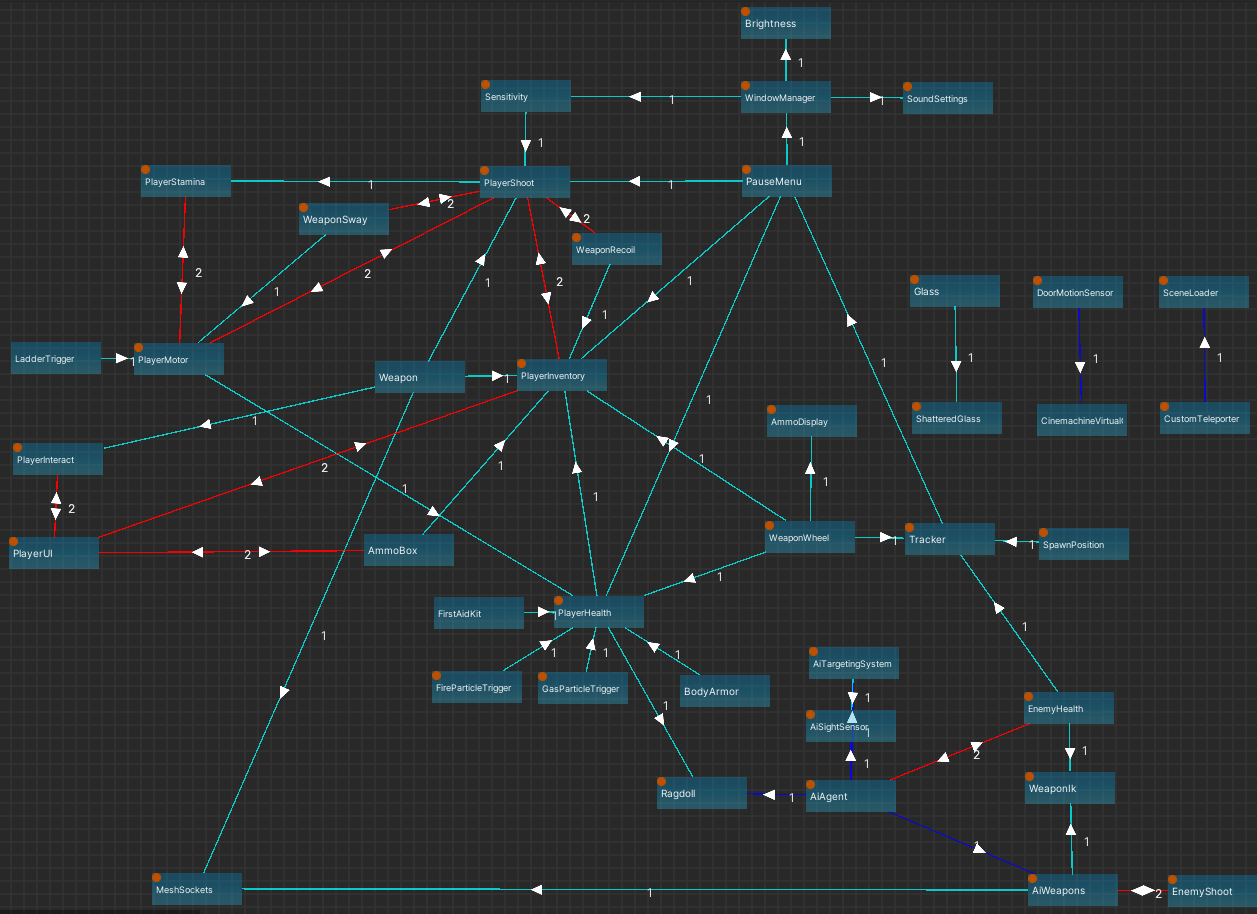
\includegraphics{Images/modulesDependency.png}
    \caption{Komunikacja między modułami}
\end{figure}
\FloatBarrier
\subsection{Wzorce projektowe}
W tym podrozdziale opiszemy, w jaki sposób konkretne wzorce projektowe są wykorzystywane w architekturze gry, jakie korzyści przynoszą, oraz jak wpływają na rozwój i utrzymanie kodu. To pozwoli Wam lepiej zrozumieć, dlaczego i w jaki sposób dany wzorzec jest stosowany w kontekście \textit{Operation Deratization}.

\subsubsection{Wzorzec szablonu metody}\label{subsubsec:tempMeth}
Wzorzec szablonu metody jest używany, gdy algorytm ma pewne kroki wspólne, ale pewne kroki są specyficzne dla konkretnych podklas. Poniżej znajduje się implementacja wzorca szablonu metody w klasie \texttt{Interactable}:
\begin{codebox}
\begin{lstlisting}[language={[Sharp]C}, label={listing:Interactable.cs}]
public abstract class Interactable : MonoBehaviour
{
    [Header("Interactables")]
    public bool useEvents;
    public string prompt;

    public virtual string OnLook()
    {
        return prompt;
    }
    public void BaseInteract()
    {
        if (useEvents)
            GetComponent<InteractionEvent>().OnInteract.Invoke();

        Interact();
    }
    protected virtual void Interact()
    {

    }
}
\end{lstlisting}
\end{codebox}
\captionof{lstlisting}{Klasa Interactable, z której dziedziczą wszystkie skrypty interaktywnych obiektów w grze}
Wzorzec szablonu metody (\textit{Template method pattern}): Metoda \texttt{BaseInteract} jest szablonem, a metoda \texttt{Interact} jest hookiem (hakiem), który może być nadpisywany przez klasy dziedziczące. Dzięki temu, wspólne kroki interakcji są zdefiniowane w klasie bazowej (\texttt{Interactable}), ale specyficzne zachowanie może być dostosowane przez podklasy.

\subsubsection{Wzorzec stanu}\label{subsubsec:state}
Wzorzec stanu jest używany, gdy obiekt ma zmieniające się zachowanie w zależności od swojego stanu wewnętrznego. Poniżej znajduje się implementacja wzorca stanu w klasie \texttt{AiState}:
\begin{codebox}
\begin{lstlisting}[language={[Sharp]C}, label={listing:AiState.cs}]
public enum AiStateId
{
    ChasePlayer,
    Death,
    Idle,
    FindWeapon,
    AttackTarget,
    FindTarget,
    FindFirstAidKit,
    FindAmmo
}
public interface AiState
{
    AiStateId GetId();

    void Enter(AiAgent agent);
    void Update(AiAgent agent);
    void Exit(AiAgent agent);
}
\end{lstlisting}
\end{codebox}
\captionof{lstlisting}{Implementacja wzorca stanu w klasie AiState}
Wzorzec stanu (\textit{State pattern}): W tym przypadku, enum \texttt{AiStateId} reprezentuje różne stany, a interfejs \texttt{AiState} definiuje operacje związane z każdym stanem (\texttt{Enter}, \texttt{Update}, \texttt{Exit}). Każdy stan implementuje ten interfejs, co pozwala obiektowi AI zmieniać swoje zachowanie dynamicznie, w zależności od aktualnego stanu.

\subsubsection{Wzorzec puli obiektów} \label{subsubsec:objPoolPattern}
Wzorzec puli obiektów został zaimplementowany w klasie \texttt{ObjectPoolManager}, która zarządza efektywnym ponownym użyciem obiektów, minimalizując koszty tworzenia i usuwania. Kluczowe funkcje obejmują dynamiczne tworzenie pul obiektów, efektywne tworzenie i zwracanie obiektów. Poniżej znajdziesz implementację wzorca puli obiektów:
\begin{codebox}
\begin{lstlisting}[language={[Sharp]C}]
public class ObjectPoolManager : MonoBehaviour
{
    // ... (Remaining part of the script)

    public static GameObject SpawnObject(GameObject objectToSpawn, Vector3 spawnPosition, Quaternion spawnRotation, PoolType poolType)
    {
        PooledObjectInfo pool = null;
        
        foreach (PooledObjectInfo p in ObjectPools)
        {
            if (p.LookupString == objectToSpawn.name)
            {
                pool = p;
                break;
            }
        }
        
        if (pool == null)
        {
            pool = new PooledObjectInfo() { LookupString = objectToSpawn.name };
            ObjectPools.Add(pool);
        }
        
        GameObject spawnableObj = pool.InactiveObjects.FirstOrDefault();
        
        if (spawnableObj == null)
        {
            GameObject parentObject = SetParentObject(poolType);
            spawnableObj = Instantiate(objectToSpawn, spawnPosition, spawnRotation);
            spawnableObj.transform.SetParent(parentObject.transform);
        }
        else
        {
            spawnableObj.transform.position = spawnPosition;
            spawnableObj.transform.rotation = spawnRotation;
            pool.InactiveObjects.Remove(spawnableObj);
            spawnableObj.SetActive(true);
        }
        
        return spawnableObj;
    }

    // ... (Remaining part of the script)
}
\end{lstlisting}
\end{codebox}
\captionof{lstlisting}{Klasa ObjectPoolManager odpowiedzialna za tworzenie pul obiektów}
\begin{codebox}
\begin{lstlisting}[language={[Sharp]C}]
public class ObjectPoolManager : MonoBehaviour
{
    // ... (Remaining part of the script)

    public static void ReturnObjectToPool(GameObject obj)
    {
        string objName = obj.name.Substring(0, obj.name.Length - 7);
        PooledObjectInfo pool = null;

        foreach (PooledObjectInfo p in ObjectPools)
        {
            if (p.LookupString == objName)
            {
                 pool = p;
                 break;
            }
        }

        if (pool == null)
            Debug.LogWarning("Trying to release an object that is not pooled: " + obj.name);
        else
        {
            obj.SetActive(false);
            pool.InactiveObjects.Add(obj);
        }
    }

    // ... (Remaining part of the script)
}
\end{lstlisting}
\end{codebox}
\captionof{lstlisting}{Fragment skryptu ObjectPoolManager.cs używany do zwracania obiektów do puli obiektów}
Wzorzec puli obiektów (\textit{State pattern}): W klasie \texttt{ObjectPoolManager} jest szeroko wykorzystywany do efektywnego zarządzania obiektami w grze, poprawiając wydajność i optymalizując zużycie pamięci. Jeżeli interesują Cię konkretne przykłady użycia tego wzorca zachęcamy do kliknięcia w odnośnik, który skieruje Cię do rozdziału o optymalizacji, gdzie szerzej opisaliśmy zalety stosowania tej techniki:  \nameref{subsubsec:objPoolExamples}

\newpage

\section{Interfejs użytkownika (UI) i grafika}\label{sec:ui}
W tej sekcji skoncentrujemy się na omówieniu kluczowych aspektów związanych z projektowaniem interfejsu użytkownika (UI) oraz doświadczenia użytkownika (UX), wraz z procesem tworzenia grafik dedykowanych do gry. Krok po kroku przewodniczyć będziemy przez projektowanie zarówno interaktywnego Menu Głównego, jak i ekranów w trakcie rozgrywki (Ingame).

Pierwszym etapem naszej analizy będzie zgłębienie szczegółów dotyczących UI i UX, identyfikując kluczowe elementy, które wpłyną pozytywnie na doświadczenie użytkownika. Starannie przyjrzymy się interaktywnym funkcjom, które mają być zawarte zarówno w Menu Głównym, jak i w trakcie samej rozgrywki, dążąc do stworzenia intuicyjnego i przyjaznego środowiska dla gracza.

Następnie skupimy się na procesie projektowania grafik, uwzględniając zarówno estetykę, jak i funkcjonalność. Przeanalizujemy style graficzne oraz czcionki, z myślą o tworzeniu spójnego i atrakcyjnego wizualnie interfejsu. Warto podkreślić, że każdy element graficzny będzie starannie dopasowany, aby nie tylko efektywnie przyciągnąć uwagę gracza, ale również ułatwić nawigację i zrozumienie dostępnych opcji.

Podsumowując, naszym celem jest stworzenie UI i UX, które nie tylko spełnią oczekiwania co do estetyki, ale przede wszystkim będą funkcjonalne i przyjazne dla gracza. Prześledzimy proces od projektowania do finalnej implementacji, dbając o każdy detal, aby zapewnić satysfakcję i wygodę użytkownikowi podczas eksploracji Menu Głównego oraz w trakcie fascynującej rozgrywki.
\subsection{Projektowanie interfejsu użytkownika}
W trakcie projektowania interfejsu użytkownika (UI) kluczowe jest osiągnięcie równowagi pomiędzy estetyką a funkcjonalnością. Oprócz estetycznego designu, priorytetem jest stworzenie interfejsu, który jest intuicyjny i efektywny dla użytkowników. Proces ten obejmuje systematyczne testowanie i uwzględnianie opinii, dążąc do idealnego połączenia atrakcyjnego wyglądu z praktycznym zastosowaniem, co sprawia, że interfejs nie tylko przyciąga uwagę, ale także doskonale spełnia potrzeby użytkowników.

\subsubsection{Tworzenie logo naszej gry}
Na wstępie skoncentrujmy się na kreowaniu głównego logo naszej gry, bowiem jest to nie tylko centralny element, ale także jedno z zadań, które mimo swojej doniosłości, należy do tych bardziej dostępnych w kwestii realizacji.

Rozpoczniemy od procesu projektowania, który skupi naszą uwagę na stworzeniu identyfikacyjnego znaku graficznego gry. Traktując to jako priorytetowe zadanie, pragniemy nadać mu zarówno wyjątkowość, jak i łatwą rozpoznawalność. Celem jest opracowanie logo, które nie tylko odda charakter naszej gry, ale także wyróżni ją spośród innych.

W pierwszym etapie zwrócimy szczególną uwagę na koncepcję graficzną, starając się połączyć estetykę z funkcjonalnością. Zależy nam na tym, aby logo nie tylko zachwycało wizualnie, ale również komunikowało istotne elementy związane z tematyką gry. Podejdziemy do tego zadania z pełnym zaangażowaniem, starając się wykorzystać prostotę w projektowaniu, co z kolei sprawi, że logo będzie łatwo zapamiętywalne i zrozumiałe dla potencjalnych graczy.

W procesie tworzenia skoncentrujemy się na doskonałym dopasowaniu kolorów, kształtów i czcionek, aby osiągnąć optymalny efekt wizualny. Stworzymy coś nie tylko estetycznego, ale także trwałego i godnego reprezentowania gry na rynku.

W skrócie, celem jest opracowanie nie tylko logo, ale prawdziwej ikony charakteryzującej naszą grę, która będzie zarówno atrakcyjna wizualnie, jak i funkcjonalna w przekazywaniu istotnych informacji o produkcie.

\begin{center}
{\bfseries Główne logo}
\end{center}
\begin{figure}[h]
    \centering
    
\includegraphics[scale=15]{Images/logo.png}
    \caption{Główne logo, w którym są nawiązania do tytułu tworzonej przez nas gry}
\end{figure}
\FloatBarrier

W centralnym punkcie kompozycji wyróżnia się kontur szczura, symbolicznego odniesienia do graczy na mapie, określanych w potocznym żargonie jako "szczury". Wybór tego motywu wynika z naszej koncepcji, która nawiązuje do najbardziej niebezpiecznych postaci z różnych więzień i środowisk. W świecie gry, gracz zostaje postawiony przed zadaniem eliminacji tych "szczurów", reprezentujących najbardziej zróżnicowane i złożone przestępcze postacie. Ostatecznym celem jest perfekcyjne zrealizowanie brutalnej rozgrywki, eliminując wszystkich przeciwników i upewniając się, że żaden z nich nie przeżyje starcia.
Przyjęcie motywu szczura jako symbolu podkreśla nie tylko surowość środowiska przedstawionego w grze, ale także wprowadza unikalny aspekt, który stanowi istotny element narracyjny. Szczury, jako metafora najbardziej zaciekłych przeciwników, dodają głębię fabularną oraz wywołują emocje związane z koniecznością pokonania skomplikowanego i nieprzewidywalnego przeciwnika.

W rezultacie, widoczna sylwetka szczura na głównym planie nie tylko stanowi element graficzny, ale także istotny komponent narracyjny, wzbogacający doświadczenie gracza poprzez ukazanie surowości oraz wyzwania, jakie stawia przed nim świat gry.\\

\subsubsection{Tworzenie logo Menu głównego}

Po stworzeniu głównego logo gry skoncentrujemy się na opracowaniu grafiki do menu głównego. W tym procesie zwrócimy szczególną uwagę na aspekty wizualne, aby logo doskonale wpasowało się w ogólny wygląd i tematykę gry. Naszym celem jest nie tylko estetyczna prezentacja w menu, ale także harmonijne zintegrowanie logotypu, tworząc spójną wizualną całość. Poprzez analizę detali kompozycji, kolorów i proporcji, dążymy do uzyskania efektu, który przyciągnie uwagę graczy i skutecznie przekazywać będzie charakter gry. Proces ten obejmie staranne dostosowanie grafiki do kontekstu menu, tworząc przyjemne wrażenie wizualne już na pierwszym spotkaniu gracza z grą.
\begin{center}
\end{center}
\begin{figure}[h]
    \centering
    
\includegraphics[scale=0.2]{Images/mainLogo.jpg}
    \caption{Logo w głównym Menu, domyślnie jest z przezroczystym tłem (w tym przypadku tło dodane po ukończeniu logo)}
\end{figure}

Na przedstawionej grafice zauważamy, że logo zostało zręcznie wkomponowane jako litera w tytule gry. Ten subtelny zabieg nie tylko stanowi estetyczny atut dla oka, ale także wyróżnia się doskonałą czytelnością, nie dominując nad pozostałymi elementami. Stworzone w ten sposób logo idealnie komponuje się z ogólnym układem graficznym, prezentując równowagę między atrakcyjnym wyglądem a funkcjonalnością.

W trakcie tworzenia menu głównego gry planujemy skorzystać z tego logo, umieszczając je w sposób, który będzie sprzyjał spójności i łatwości odczytu dla graczy. Intencją jest stworzenie Main Menu, które nie tylko będzie wizualnie atrakcyjne, ale również praktyczne, umożliwiając płynną nawigację i dostarczając przyjemnego doświadczenia użytkownika od samego początku interakcji z grą.\\

\subsubsection{Main Menu}
Nadszedł moment, aby przystąpić do projektowania menu głównego naszej gry. W tym celu stworzyliśmy wstępny, aczkolwiek szczegółowy szkic, korzystając z popularnych narzędzi graficznych. Ten etap obejmuje opracowanie koncepcji, układu i funkcji, które będą dostępne dla gracza na etapie rozpoczęcia gry. Stworzyliśmy schematyczny rysunek, który stanowi swoiste mapowanie wizualne tego, jak zamierzamy zorganizować interakcję użytkownika z grą, uwzględniając zarówno estetyczne aspekty, jak i praktyczne potrzeby użytkowników.

W tym procesie zwracamy uwagę na czytelność, intuicyjność nawigacji oraz estetyczne dopasowanie do ogólnej koncepcji gry. Wszystko to ma na celu stworzenie menu głównego, które nie tylko przyciągnie uwagę graczy swoim wyglądem, ale również zapewni im łatwą i satysfakcjonującą interakcję z grą od samego początku.

\begin{figure}[h]
\begin{center}
{\bfseries Rysunek schematyczny menu}
\end{center}
    \centering
    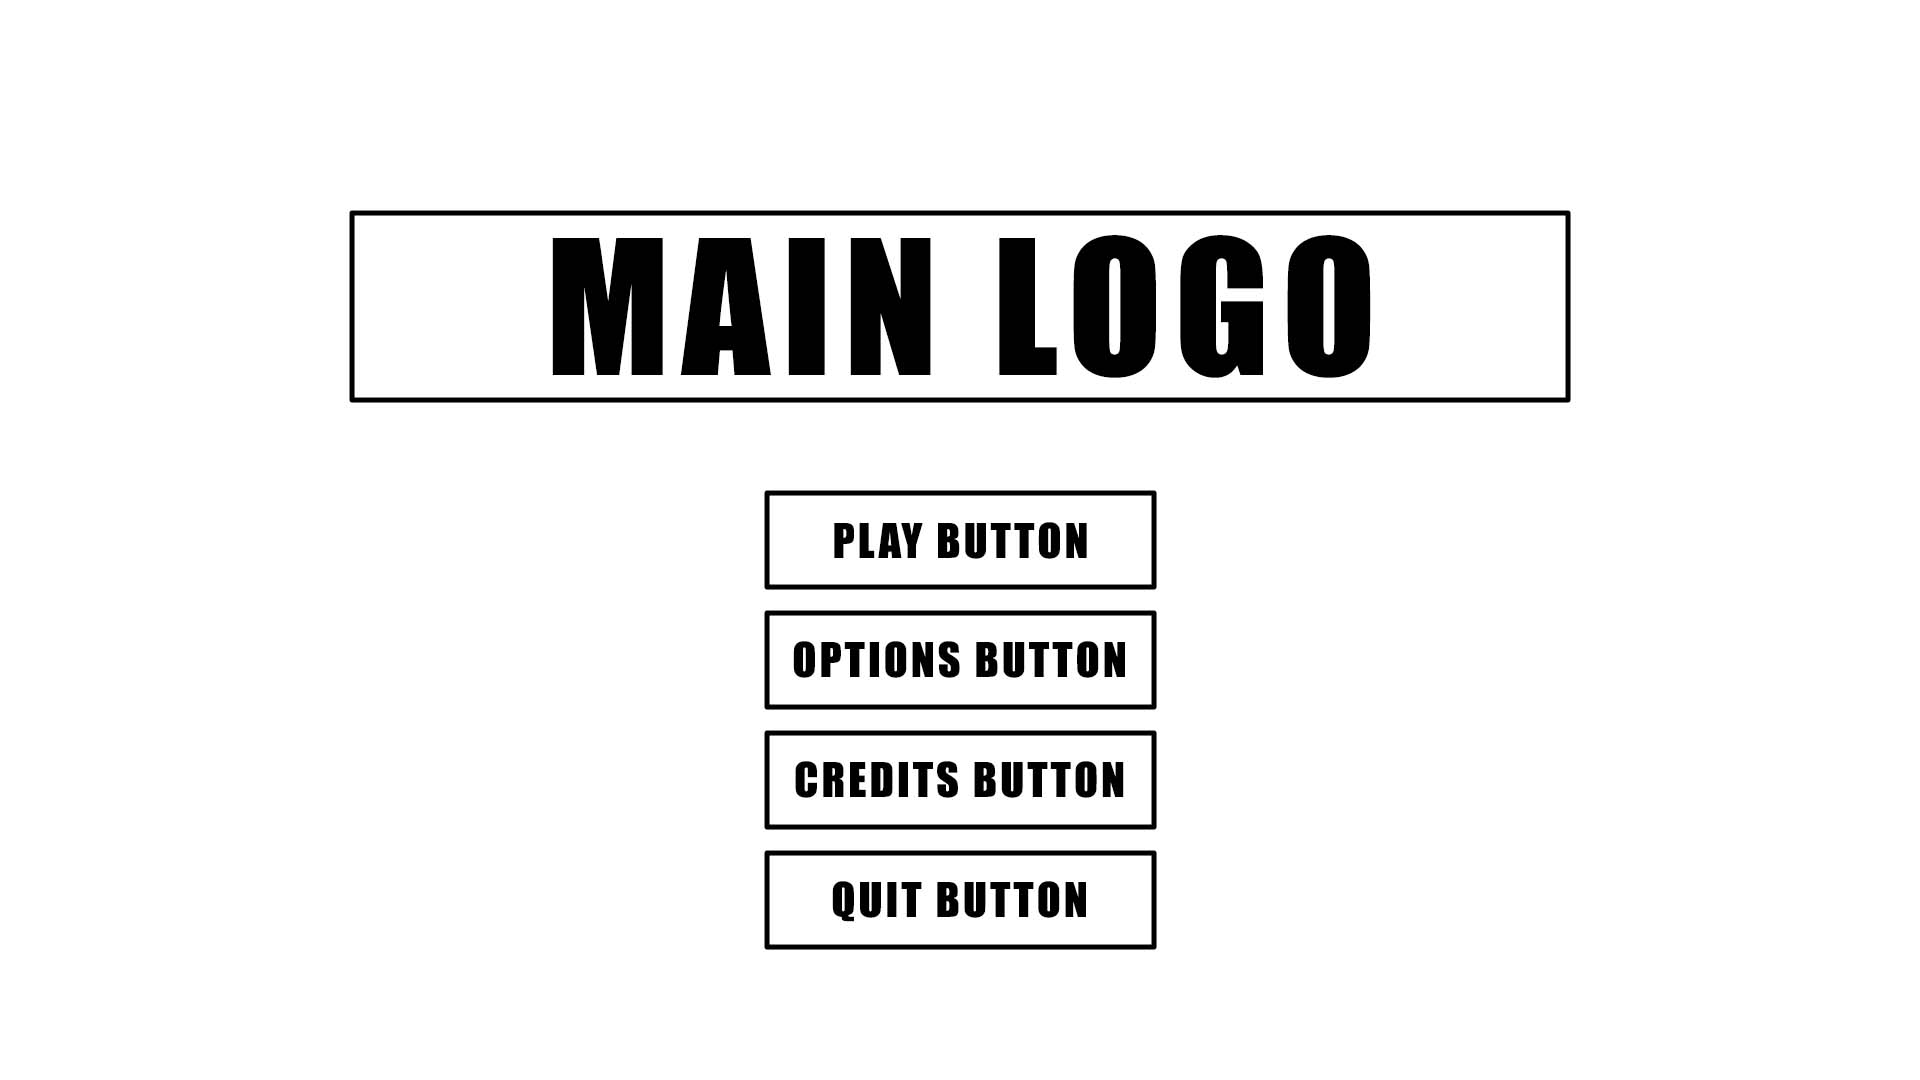
\includegraphics[scale=0.2]{Images/templateMenu.jpg}
    \caption{Na powyższym obraz możemy zobaczyć bardzo uproszczony rysunek schematyczny z procesów tworzenia Menu}
\end{figure}
\FloatBarrier

Po akceptacji wszystkich członków teamu możemy zacząć tworzenie naszego projektu w grze.

\begin{figure}[h]
\begin{center}
{\bfseries Gotowe Main Menu - w grze}
\end{center}
    \centering
    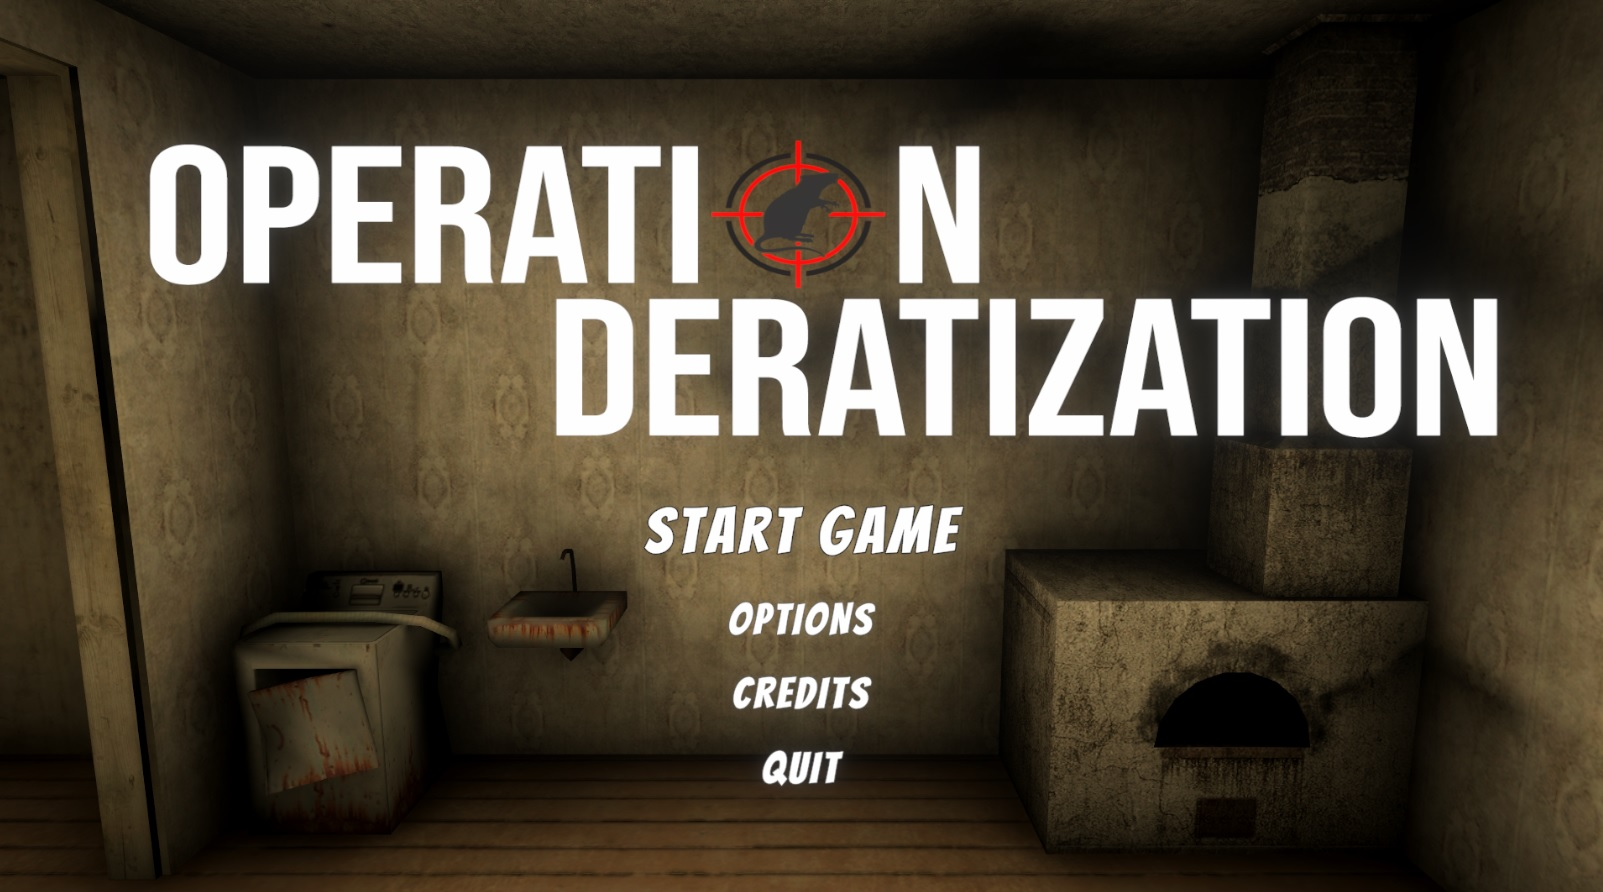
\includegraphics[width=0.75\linewidth]{Images/mainMenuInGame.jpg}
    \caption{Nasze Main Menu utworzone już w grze}
\end{figure}
\FloatBarrier

Tworzenie zaczynamy od zrobienia sceny, na której ustawiliśmy dom, w którym znajduje się całość naszego Menu. Wokół postawiliśmy drzewa, które pełnią formę estetyczną, ponieważ wszystko widać przez okna a nie chcemy aby była widoczna pusta przestrzeń. Następnie w naszym budynku planujemy i tworzymy wnętrze, dodajemy kilka assetów aby nie świeciło ono pustkami. Jak możemy zobaczyć sugerowaliśmy się naszym wcześniej pokazywanym rysunkiem schematycznym. W górnej części widnieje zaprojektowane logo wraz z tytułem gry, natomiast poniżej funkcjonalne przyciski, które odpowiadają przypisanym im funkcjom. Dodatkowo pozwoliliśmy sobie dodać osobną planszę wraz z wyróżnieniem twórców gry znajdującą się pod przyciskiem "credits".\\

\begin{figure}[h]
\begin{center}
{\bfseries Credits - w grze}
\end{center}
    \centering
    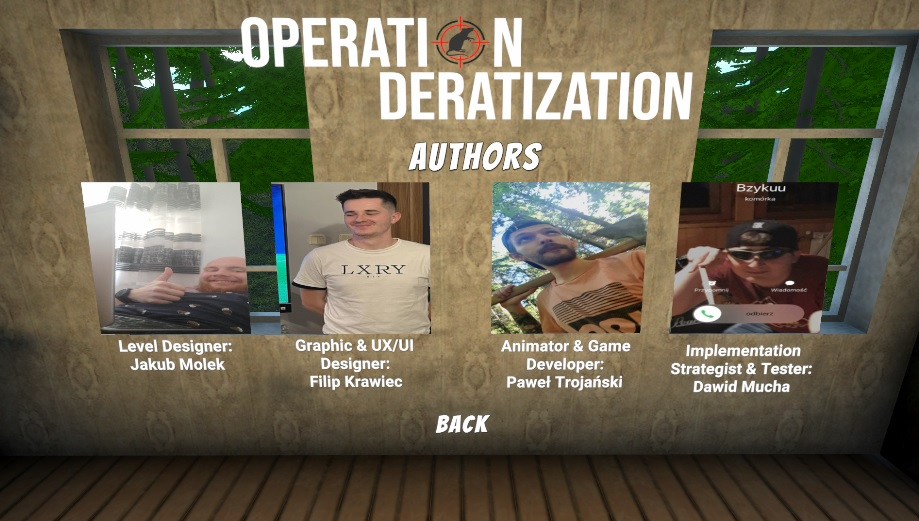
\includegraphics[width=0.75\linewidth]{Images/CreditsInGame.jpg}
    \caption{Plansza "Credits"}
\end{figure}

Jak możemy zobaczyć na powyższym obrazku plansza "Credits" zawiera informacje o autorach gry. W tle możemy zobaczyć wcześniej wspominane drzewa, które elegancko wypełniają na pustą przestrzeń na terenie przygotowanym pod Main Menu, w górnej części możemy zobaczyć również logo, które występuje w głównej planszy Menu. Poniżej znajdują się zdjęcia wraz z danymi autorów oraz w postaci dodatkowego smaczka mamy także przypisane do nich odpowiednie role przy tworzeniu gry. przyciskiem "Back" znajdującym się na dole strony wracamy do głównej planszy naszego menu, gdzie możemy wejść w opcje naszej gry bądź z niej wyjść.\\

\begin{figure}[h]
    \begin{center}
    {\bfseries Options - w grze}
    \end{center}
    \centering
    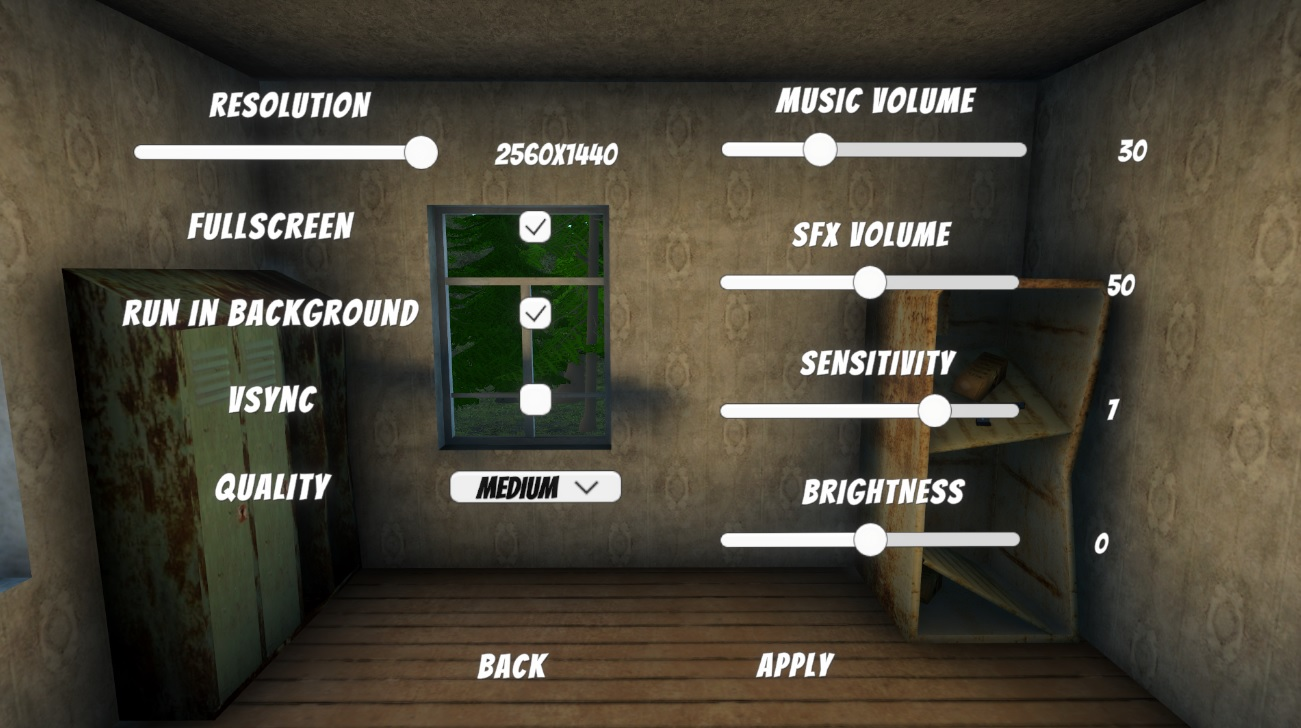
\includegraphics[width=0.75\linewidth]{Images/menuUpdated.jpg}
    \caption{Plansza "Options"}
    \begin{flushleft}
    Kolejną pozycją na naszej liście przycisków są opcje gry. Tutaj możemy zmienić wiele aspektów naszej gry, począwszy od wersji graficznej, przechodząc do akustycznej i kończywszy na indywidualnych preferencjach ustawień takich jak czułość czy używanie pełnego ekranu. Poniżej znajdują się dwa przyciski, po naciśnięciu przycisku \textit{Apply} wyskakuje nam okienko potwierdzenia (czy na pewno chcemy zapisać ustawienia gry), oraz po naciśnięciu przycisku \textit{Back}, tak jak w poprzednim przypadku cofamy się do głównej planszy naszego Menu.\\
    \end{flushleft}
\end{figure}
\FloatBarrier
\begin{figure}[h]
\begin{center}
{\bfseries Quit - w grze}
\end{center}
    \centering
    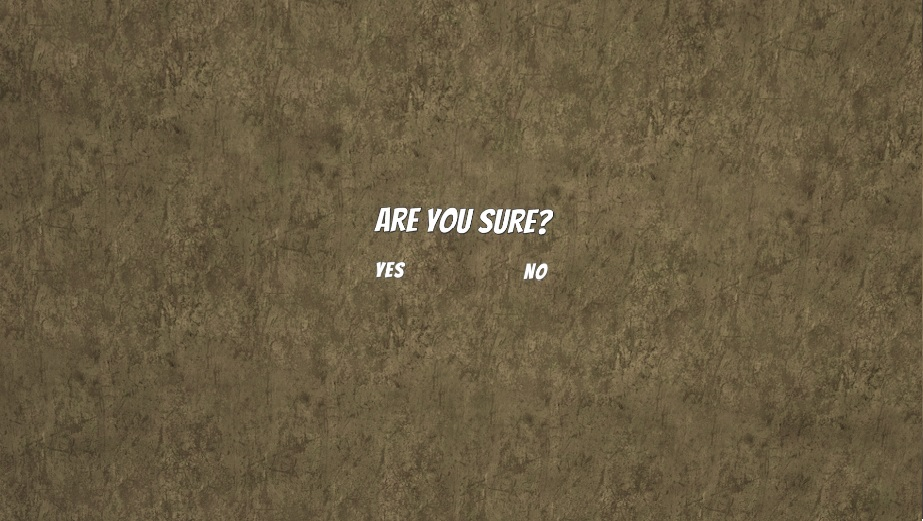
\includegraphics[width=0.75\linewidth]{Images/QuitInGame.jpg}
    \caption{Plansza "Quit"}
\end{figure}
\FloatBarrier

Jest to jedna z najprostszych i najbardziej podstawowych plansz w naszym Menu głównym. Jej zadaniem jest upewnić się czy gracz jest pewien swojej decyzji w stu procentach. Znajdują się na niej dwa przyciski \textbf{\textit{Yes}} oraz \textbf{\textit{No}}. jak możemy się domyślać po wciśnięciu przycisku po lewej stronie, nasza gra zostanie zamknięta i przejdziemy do swojego pulpitu. Ciekawostka ten ekran także jest wykorzystywany do zapisywania ustawień z planszy "Options", o której mowa była we wcześniejszym opisie.\\

\subsubsection{Loading Screen}
Jeżeli chodzi o sam \textbf{\textit{"Loading Screen"}}, pojawiającym się np. pomiędzy Menu a samą grą. Rozpoczęliśmy od przeglądnięcia ekranów wczytywania z rozmaitych gier i na tej podstawie stworzyliśmy nasz autorski projekt.

\begin{figure}[h]
\begin{center}
{\bfseries InGame Loading Screen}
\end{center}
    \centering
    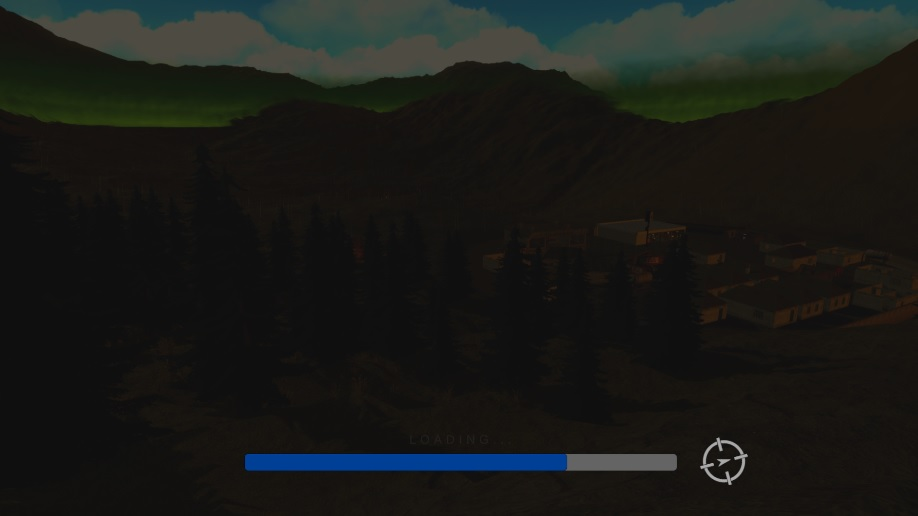
\includegraphics[width=0.75\linewidth]{Images/LoadingScreenIngame.jpg}
    \caption{Loading Screen po zaprojektowaniu i wykonaniu}
\end{figure}
\FloatBarrier

Jak możemy zobaczyć jest to jeden z podstawowych Loading Screenów. Znajduje się na nim pasek (w tym przypadku w trakcie ładowania, po prawej od paska oraz nad nim znajdują się animowany napis oraz animowana ikona naszego Trackera. W tle dodatkowo przedstawiona jest mapa, na której możemy zobaczyć przedsmak tego co się znajduje w głównej grze.

\subsubsection{InGame Pause Menu}
Istotnym elementem w doświadczeniu gracza jest "InGame Pause Menu", które można otworzyć za pomocą przycisku ESC. To istotne narzędzie zapewniające dostęp do szeregu opcji bezpośrednio w trakcie rozgrywki. W ramach tego menu, gracz ma możliwość wyjścia do menu głównego, zrestartowania rozgrywki oraz wejścia do "Ingame Options Menu". Ostatnie z wymienionych menu umożliwia dokonywanie zmian w ustawieniach gry, bez konieczności przerywania aktualnej rozgrywki.

Warto jednak zauważyć, że po wejściu do "InGame Pause Menu" gra może ulec chwilowemu zatrzymaniu, co zapewnia bezpieczne i spokojne środowisko do dokonywania zmian w ustawieniach bez pośpiechu. Ten krótkotrwały "freeze" gry jest integralną częścią procesu i zapewnia stabilność operacji dokonywanych w trakcie korzystania z "InGame Pause Menu". Dzięki tej funkcji, gracz ma pewność, że wszelkie zmiany w ustawieniach odbywają się w kontrolowany sposób, nie zakłócając płynności rozgrywki.

\begin{figure}[h]
\begin{center}
{\bfseries InGame Pause Menu}
\end{center}
    \centering
    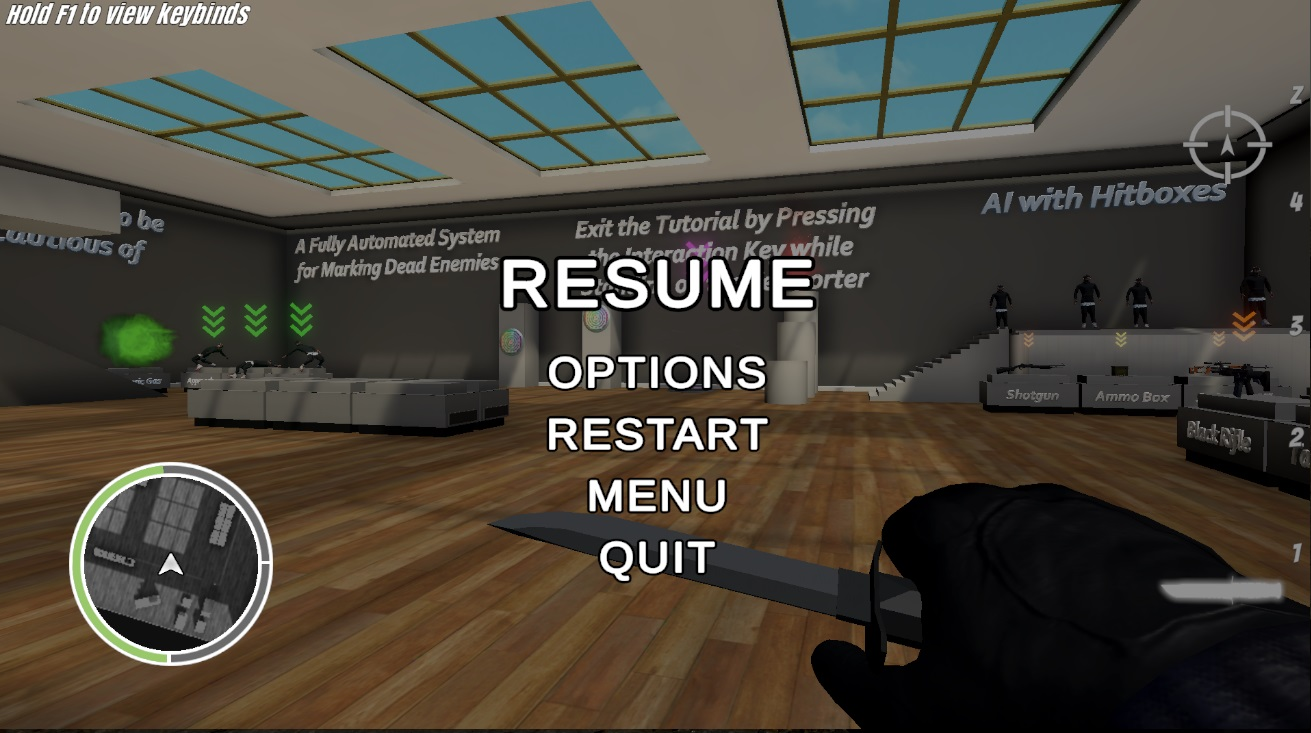
\includegraphics[width=1\linewidth]{Images/menuIngameupdated2.jpg}
        \caption{InGame Pause Menu po zaprojektu i utworzeniu}
    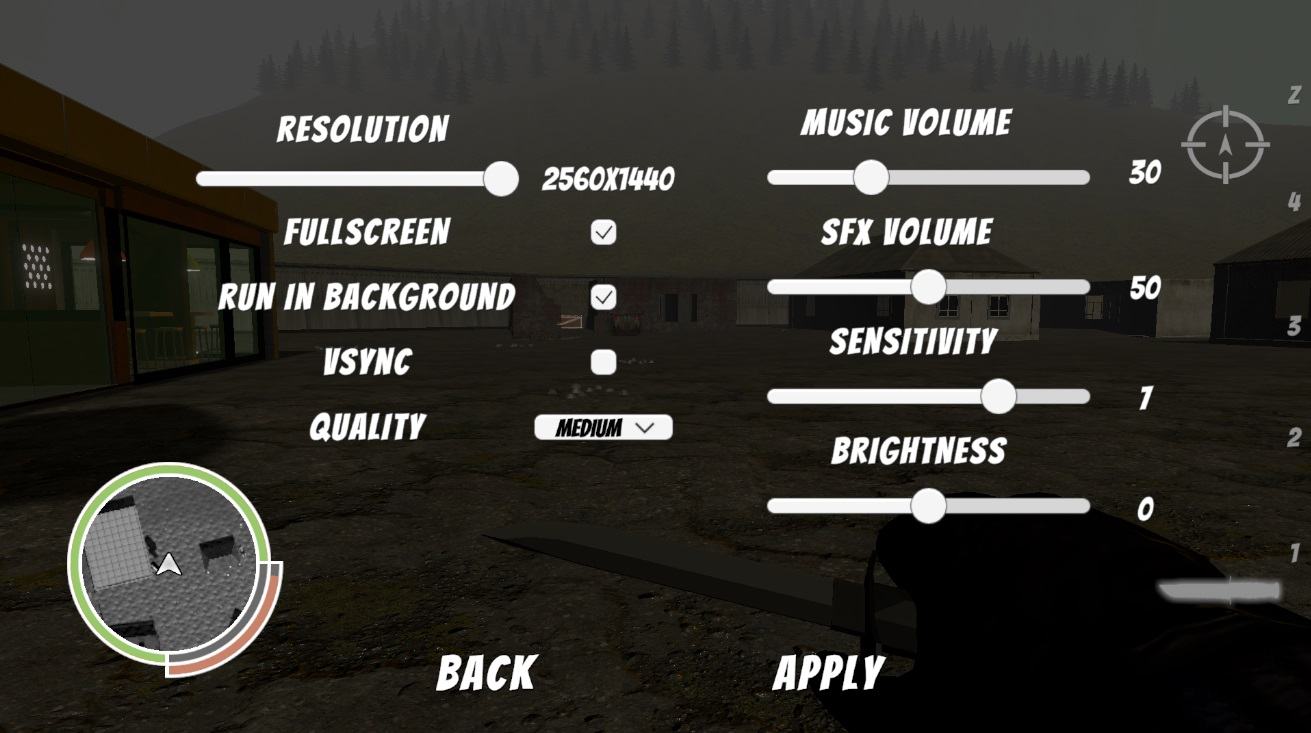
\includegraphics[width=1\linewidth]{Images/menuIngameUpdated.jpg}
    \caption{InGame Options Menu po zaprojektu i utworzeniu}
\end{figure}
\FloatBarrier

\subsubsection{Grafiki wykorzystane do Cutscenek}

Wspomniane CutSceny, czyli sekwencje filmowe w grach, stanowią niezwykle istotny element w kreowaniu bogatego narracyjnego doświadczenia. Na specjalne życzenie jednego z naszych animatorów, podjęliśmy się stworzenia kilku "memowych grafik", które stanowią kreatywną odmianę tego konwencjonalnego aspektu. Poniżej znajdują się zdjęcia przedstawiające te unikatowe grafiki, które zostały zrealizowane z myślą o dodaniu elementu humorystycznego i nieformalnego charakteru do świata gry.

Rozwinięta kreatywność w obszarze CutScen sprawia, że gracze mogą doświadczać nie tylko bogatej narracji, ale także elementów zabawy i humoru. Memowe grafiki stanowią oryginalne podejście do tego, co często bywa traktowane poważnie, dodając unikalny, lekki akcent do animacji. To przykład, jak z dbałością o detale podejście do tworzenia rozrywki może wprowadzić nową, niekonwencjonalną jakość do gier.

\begin{figure}[h]
\begin{center}
{\bfseries Cutscenes graphic}
\end{center}
    \centering
    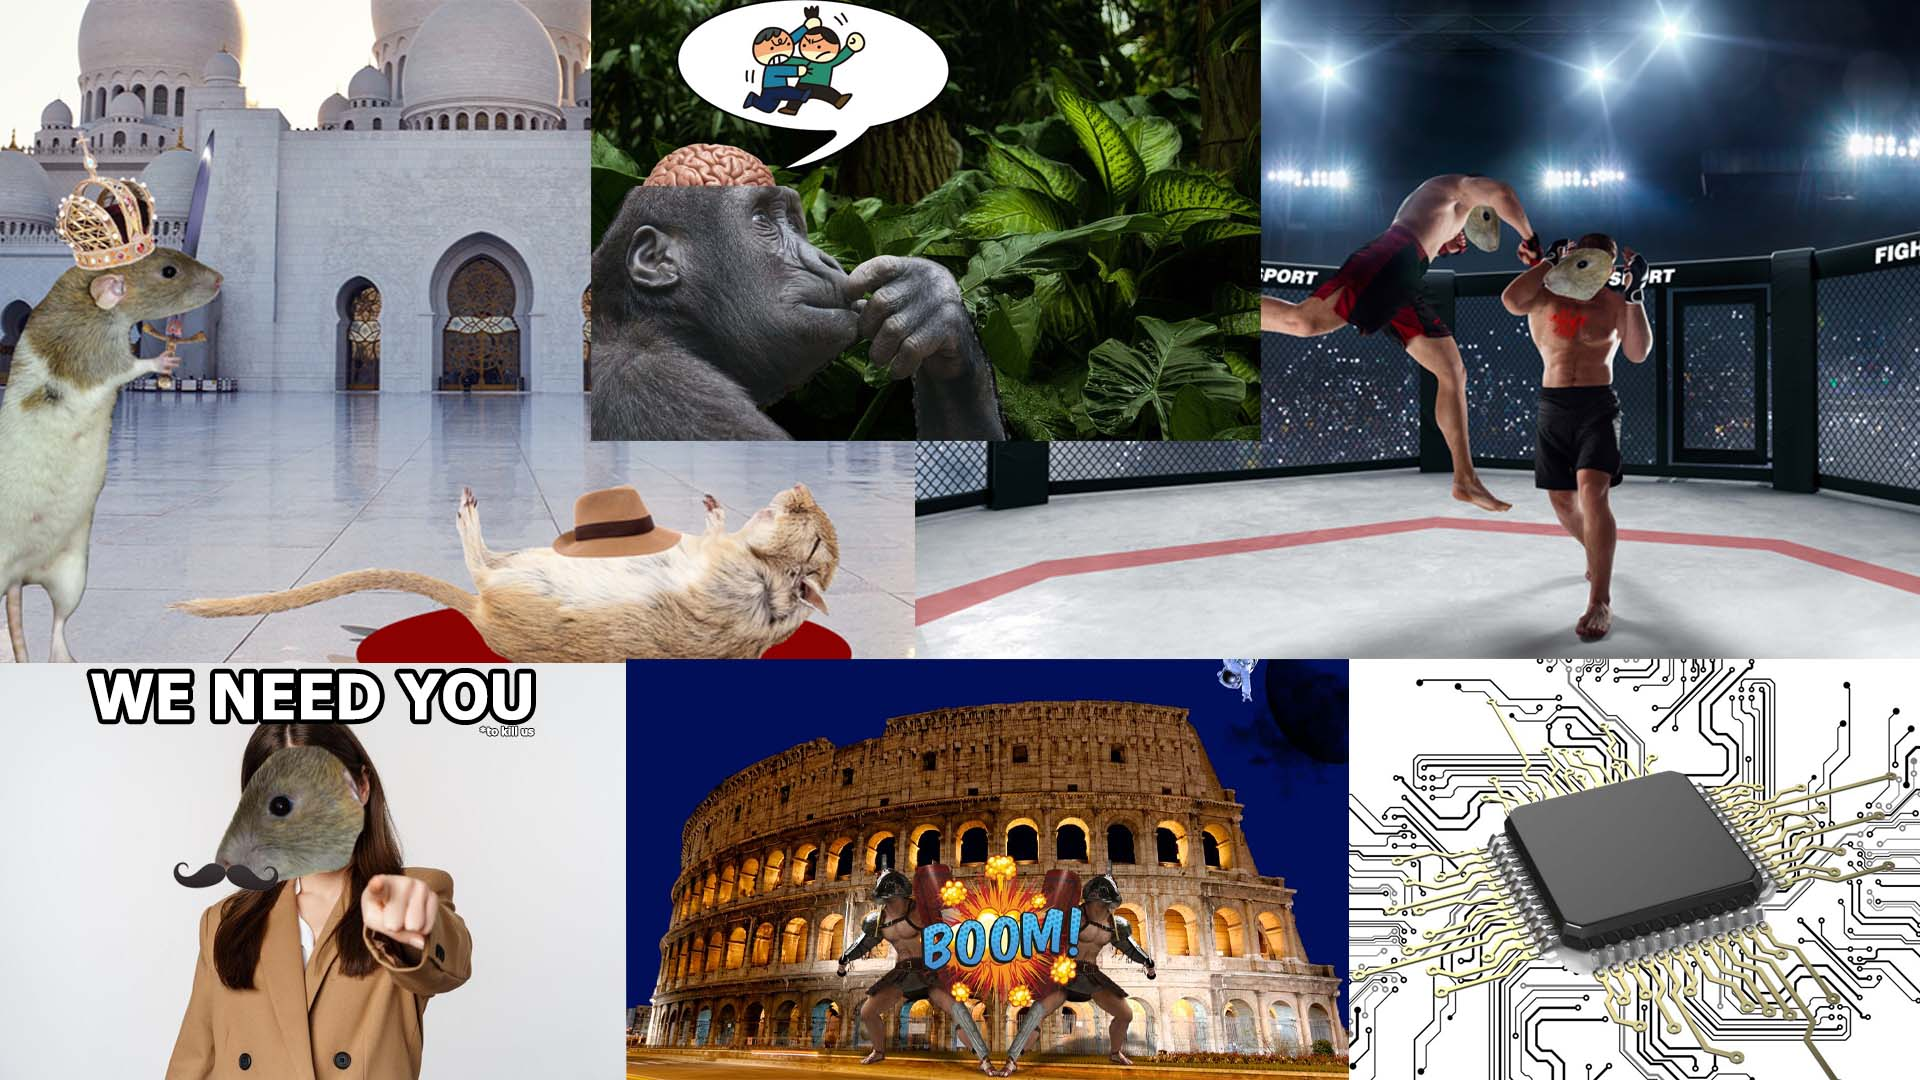
\includegraphics[width=1\linewidth]{Images/wszystkie grafiki.jpg}
        \caption{Grafiki użyte w cutscenach}
\end{figure}
\FloatBarrier

\subsection{Grafiki interfejsu}
Przechodzimy teraz do etapu przygotowywania grafiki interfejsu gracza. W tej fazie skupiamy się na opracowywaniu elementów wizualnych, które będą bezpośrednio wpływały na doświadczenie użytkownika podczas interakcji z grą. Wykorzystujemy różnorodne narzędzia graficzne, aby stworzyć estetyczne, funkcjonalne elementy, obejmujące wszystko, od ikon po przyciski i panele.

Nasz cel to nie tylko stworzenie atrakcyjnego wizualnie interfejsu, ale także dostosowanie go do ergonomicznych potrzeb graczy, zapewniając czytelność, intuicyjność i efektywność w obszarze interakcji. Grafiki interfejsu gracza będą nie tylko ozdobą, ale przede wszystkim praktycznym narzędziem, które ułatwi użytkownikom korzystanie z różnych funkcji gry, podnosząc tym samym jakość ich doświadczenia.

\subsubsection{Przygotowanie listy grafik do stworzenia}

Przygotowywanie listy grafik do stworzenia to kluczowy krok w procesie projektowania. W tym etapie identyfikujemy i szczegółowo opisujemy wszelkie grafiki, które będą niezbędne do kompleksowego stworzenia wizualnej struktury projektu. Lista ta obejmuje różnorodne elementy, takie jak logo, ikony interfejsu, tła, animacje, czy też wszelkie inne grafiki, które są istotne dla spójnego wizualnego doświadczenia użytkownika.

W trakcie tworzenia tej listy uwzględniamy zarówno elementy dekoracyjne, jak i funkcjonalne, dbając o to, aby każdy element pełnił określoną rolę w kontekście użytkowego aspektu projektu. Sprecyzowane opisy pomagają zrozumieć, jakie oczekiwania mamy co do każdej grafiki, a także ułatwiają koordynację pracy zespołu, dając klarowny plan dla artystów grafików i projektantów.

\begin{center}
{\bfseries Lista grafik do stworzenia}
\end{center}
\begin{figure}[h]
    \centering
    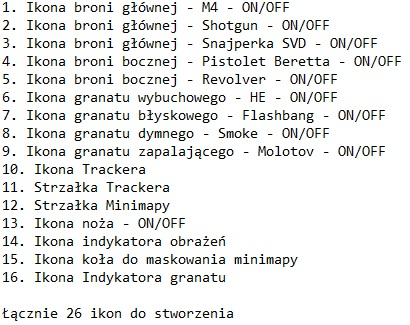
\includegraphics[scale=0.7]{Images/ListaIkon.jpg}
    \caption{Lista ikon do stworzenia}
    \label{fig:visBuglist}
\end{figure}
\FloatBarrier

\subsubsection{Poszczególne kroki tworzenia ikon}
Tutaj utworzymy ikonę, która będzie się wyświetlać podczas trzymania broni/granatu w ręku.
\begin{enumerate}
  \item Robimy screena prefabu wybranej broni. W tym przypadku Molotov.
\begin{figure}[h]
    \centering
    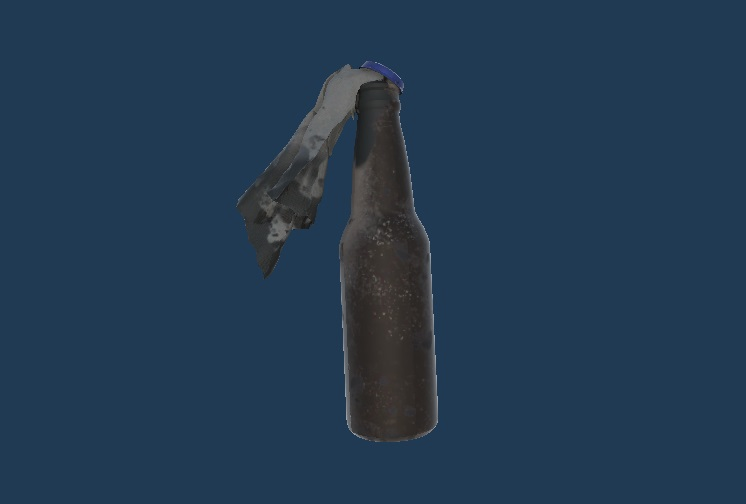
\includegraphics[scale=0.5]{Images/MolotovScreen.jpg}
    \caption{Screen prefabu}
    \label{fig:visBuglist}
\end{figure}
\FloatBarrier

  \item Wycinamy tło molotova, tak aby było przezroczyste.
\begin{figure}[h]
    \centering
    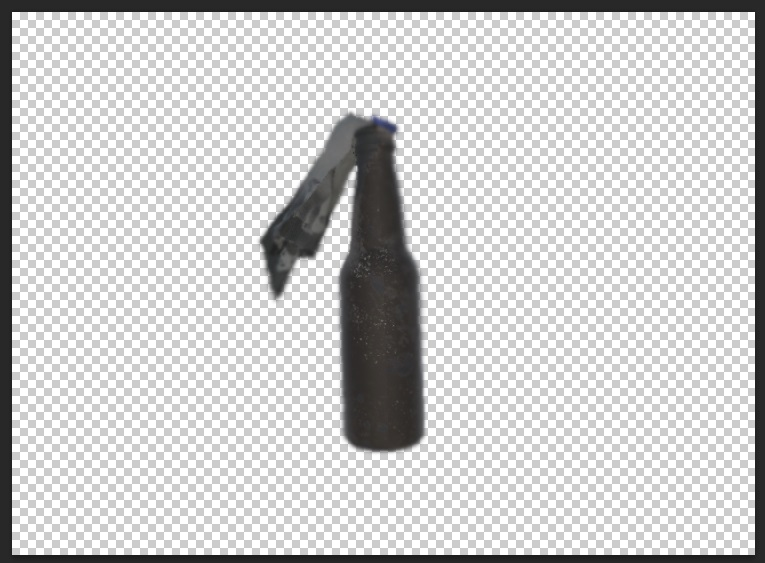
\includegraphics[scale=0.5]{Images/MolotovPNG.jpg}
    \caption{Usunięcie tła}
    \label{fig:visBuglist}
\end{figure}
\FloatBarrier

  \item Nakładamy na naszego Molotova biały kolor.
\begin{figure}[h]
    \centering
    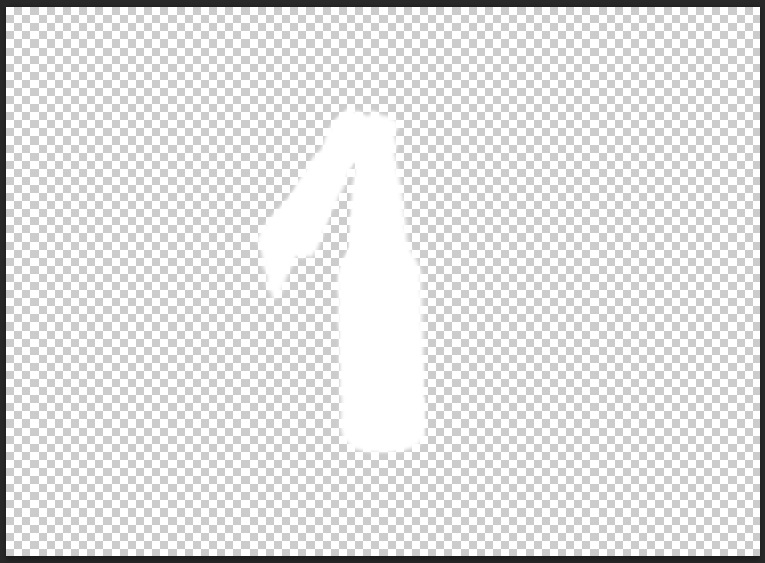
\includegraphics[scale=0.5]{Images/MolotovPNGWhite.jpg}
    \caption{Zmiana koloru na biały}
    \label{fig:visBuglist}
\end{figure}
\FloatBarrier

  \item W tym momencie nadajemy blask zewnętrzny grafice.
\begin{figure}[h]
    \centering
    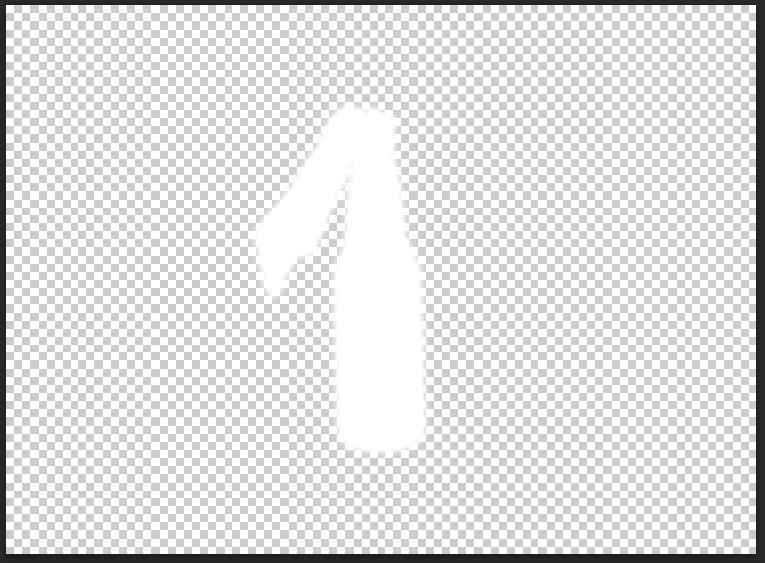
\includegraphics[scale=0.5]{Images/MolotovPNGWhiteBlask.jpg}
    \caption{Dodanie blasku zewnętrznego}
    \label{fig:visBuglist}
\end{figure}
\FloatBarrier

  \item Eksportujemy grafikę jako PNG.
\begin{figure}[h]
    \centering
    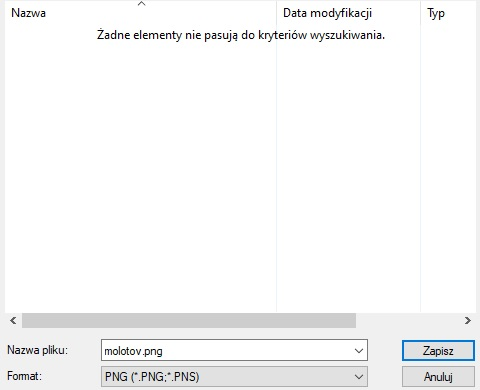
\includegraphics[scale=0.7]{Images/Saving.jpg}
    \caption{Eksport grafiki}
    \label{fig:visBuglist}
\end{figure}
\FloatBarrier
\end{enumerate}

Teraz utworzymy ikonę broni/granatu, która będzie się wyświetlała gdy posiadamy dany sprzęt bojowy w ekwipunku, ale nie trzymamy go w rękach. W tym przypadku powtarzamy \textbf{\textit{krok 1}} oraz \textbf{\textit{krok 2}}. Jeśli wykonamy poprzednie kroki możemy przystąpić do kolejnych.

\begin{enumerate}
  \item Nakładamy na naszego Molotova szary kolor.
\begin{figure}[h]
    \centering
    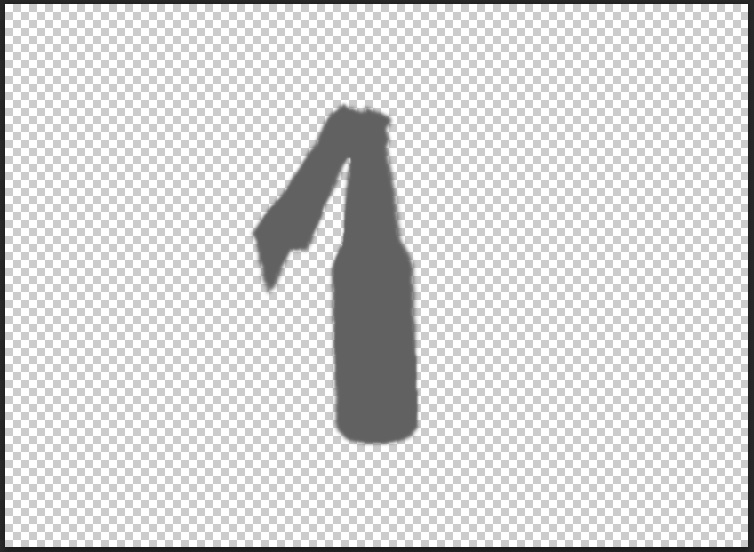
\includegraphics[scale=0.5]{Images/MolotovOFFgrey.jpg}
    \caption{Zmiana kolory na szary}
    \label{fig:visBuglist}
\end{figure}
\FloatBarrier

  \item Zmieniamy jego przezroczystość wedle upodobań.
\begin{figure}[h]
    \centering
    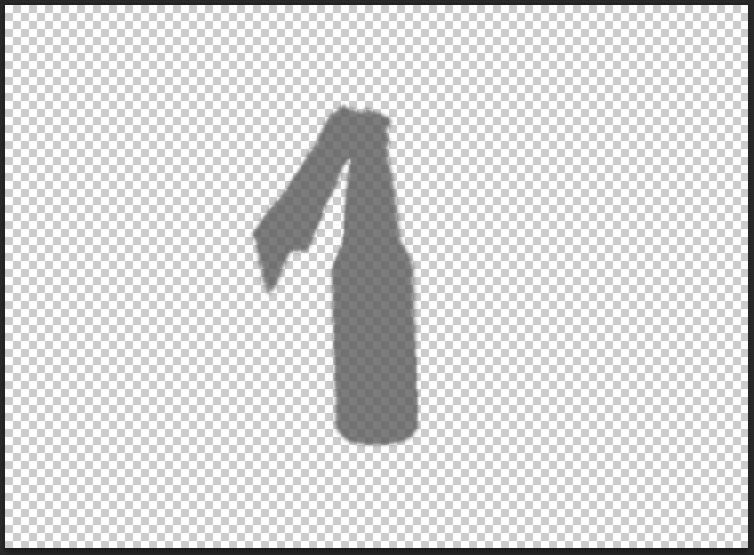
\includegraphics[scale=0.5]{Images/MolotovOFFgreyOpacity.jpg}
    \caption{Zmiana przezroczystości}
    \label{fig:visBuglist}
\end{figure}
\FloatBarrier
Jak możemy zauważyć nasze "przezroczyste" tło widać przez naszą ikonę, co oznacza, że nasza praca została wykonana pomyślnie.

  \item Eksportujemy grafikę jako PNG.
\begin{figure}[h]
    \centering
    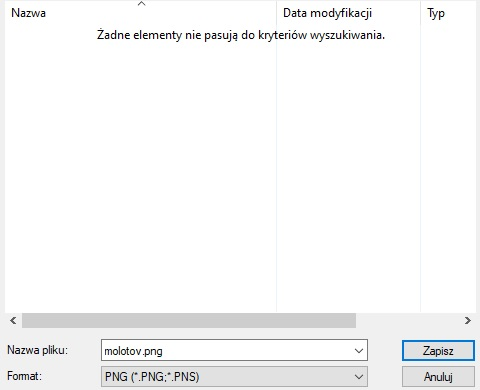
\includegraphics[scale=0.7]{Images/Saving.jpg}
    \caption{Eksport grafiki}
    \label{fig:visBuglist}
\end{figure}
\FloatBarrier
\end{enumerate}

Kolejnym krokiem jest powtórzenie tego samego procesu dla pozostałych ikon broni oraz granatów. W analogiczny sposób planujemy i tworzymy grafiki reprezentujące różne rodzaje broni oraz elementy wyposażenia, dbając o spójność wizualną z wcześniej opracowanymi elementami. Długość procesu oraz staranność w przygotowywaniu każdej ikony są kluczowe, aby zagwarantować zróżnicowanie i czytelność, jednocześnie zachowując estetyczny charakter całego zestawu. Ostatecznym celem jest stworzenie kompleksowego zestawu ikon, które będą jednoznacznie identyfikować różne elementy związane z uzbrojeniem w grze.

\subsubsection{Pokaz wszystkich granatów oraz broni zrobionych do gry}

\begin{figure}[h]
    \centering
    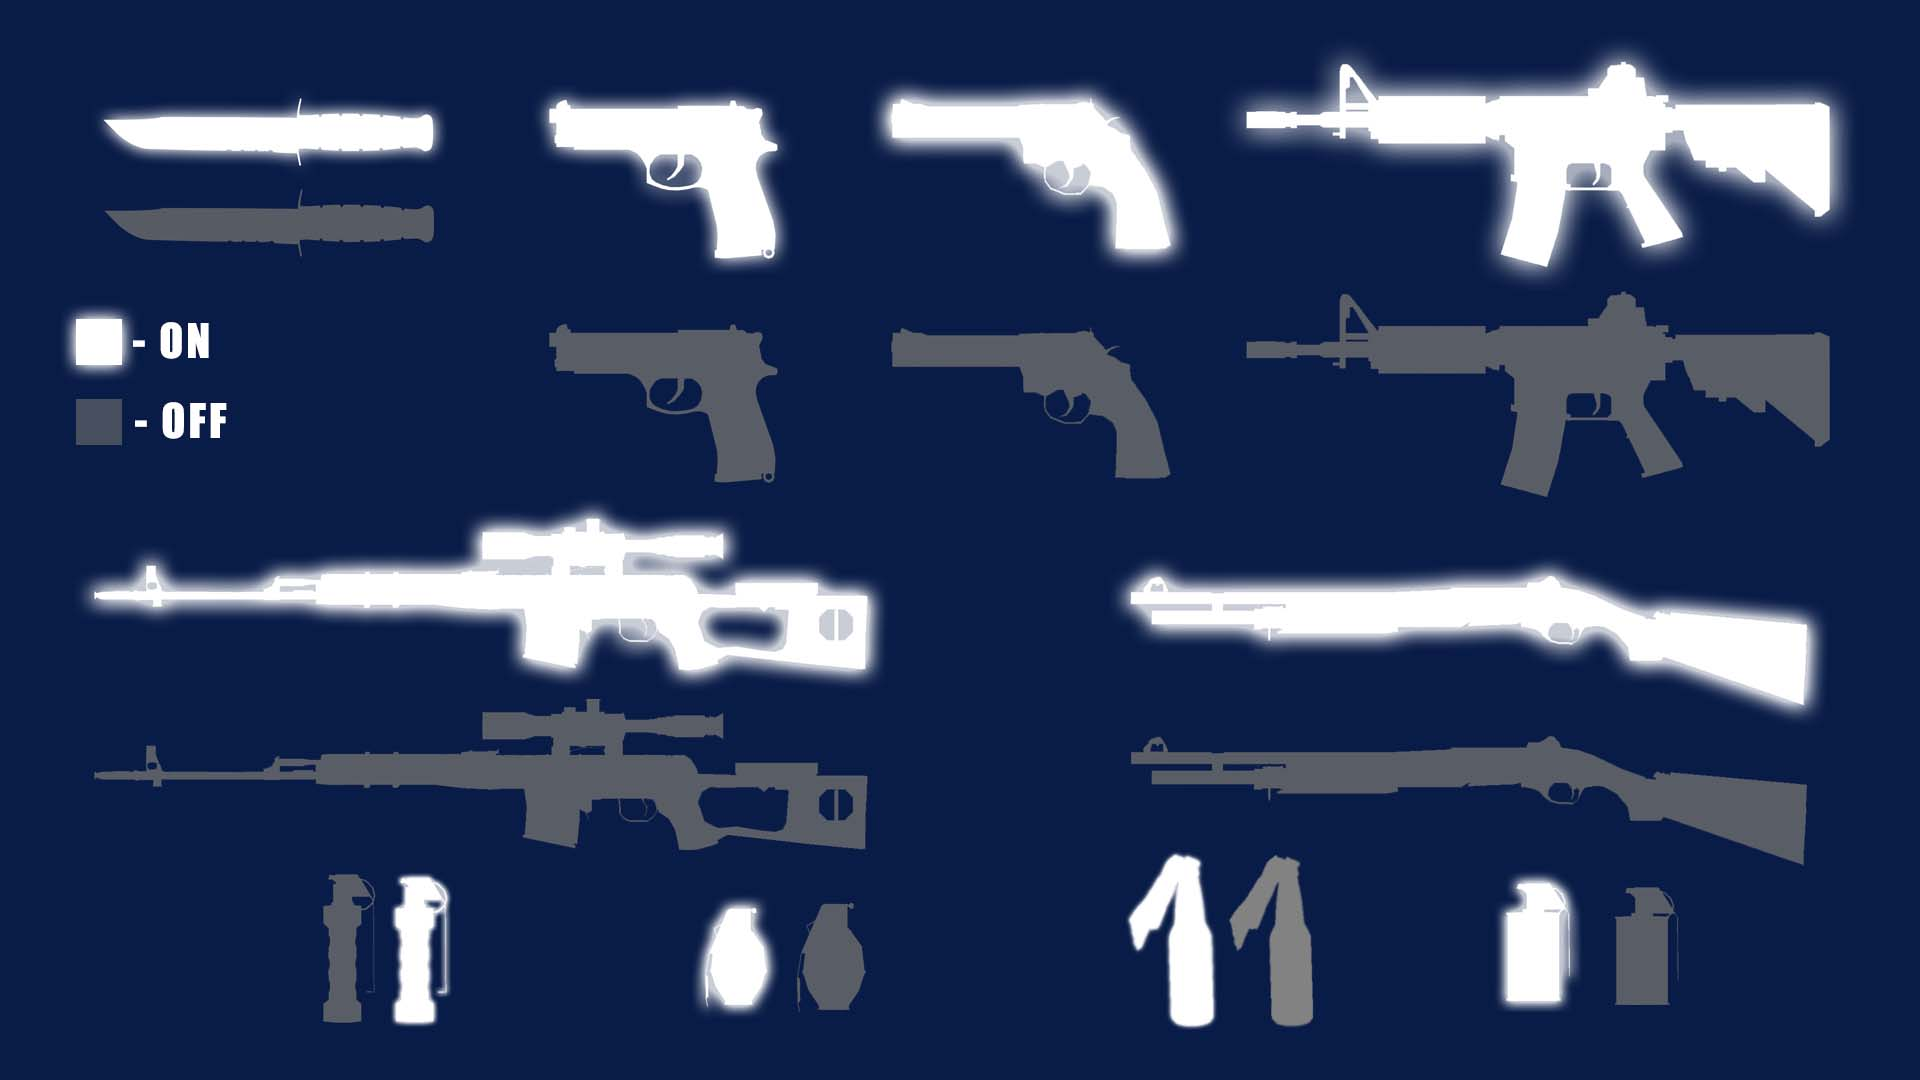
\includegraphics[scale=0.2]{Images/Pokazanie ikon broni.jpg}
    \caption{Plansza przedstawiająca wszystkie ikony broni oraz granatów w grze}
    \label{fig:visBuglist}
\end{figure}
\FloatBarrier

\subsubsection{Pokaz wszystkich ikon UI zrobionych do gry}

\begin{figure}[h]
    \centering
    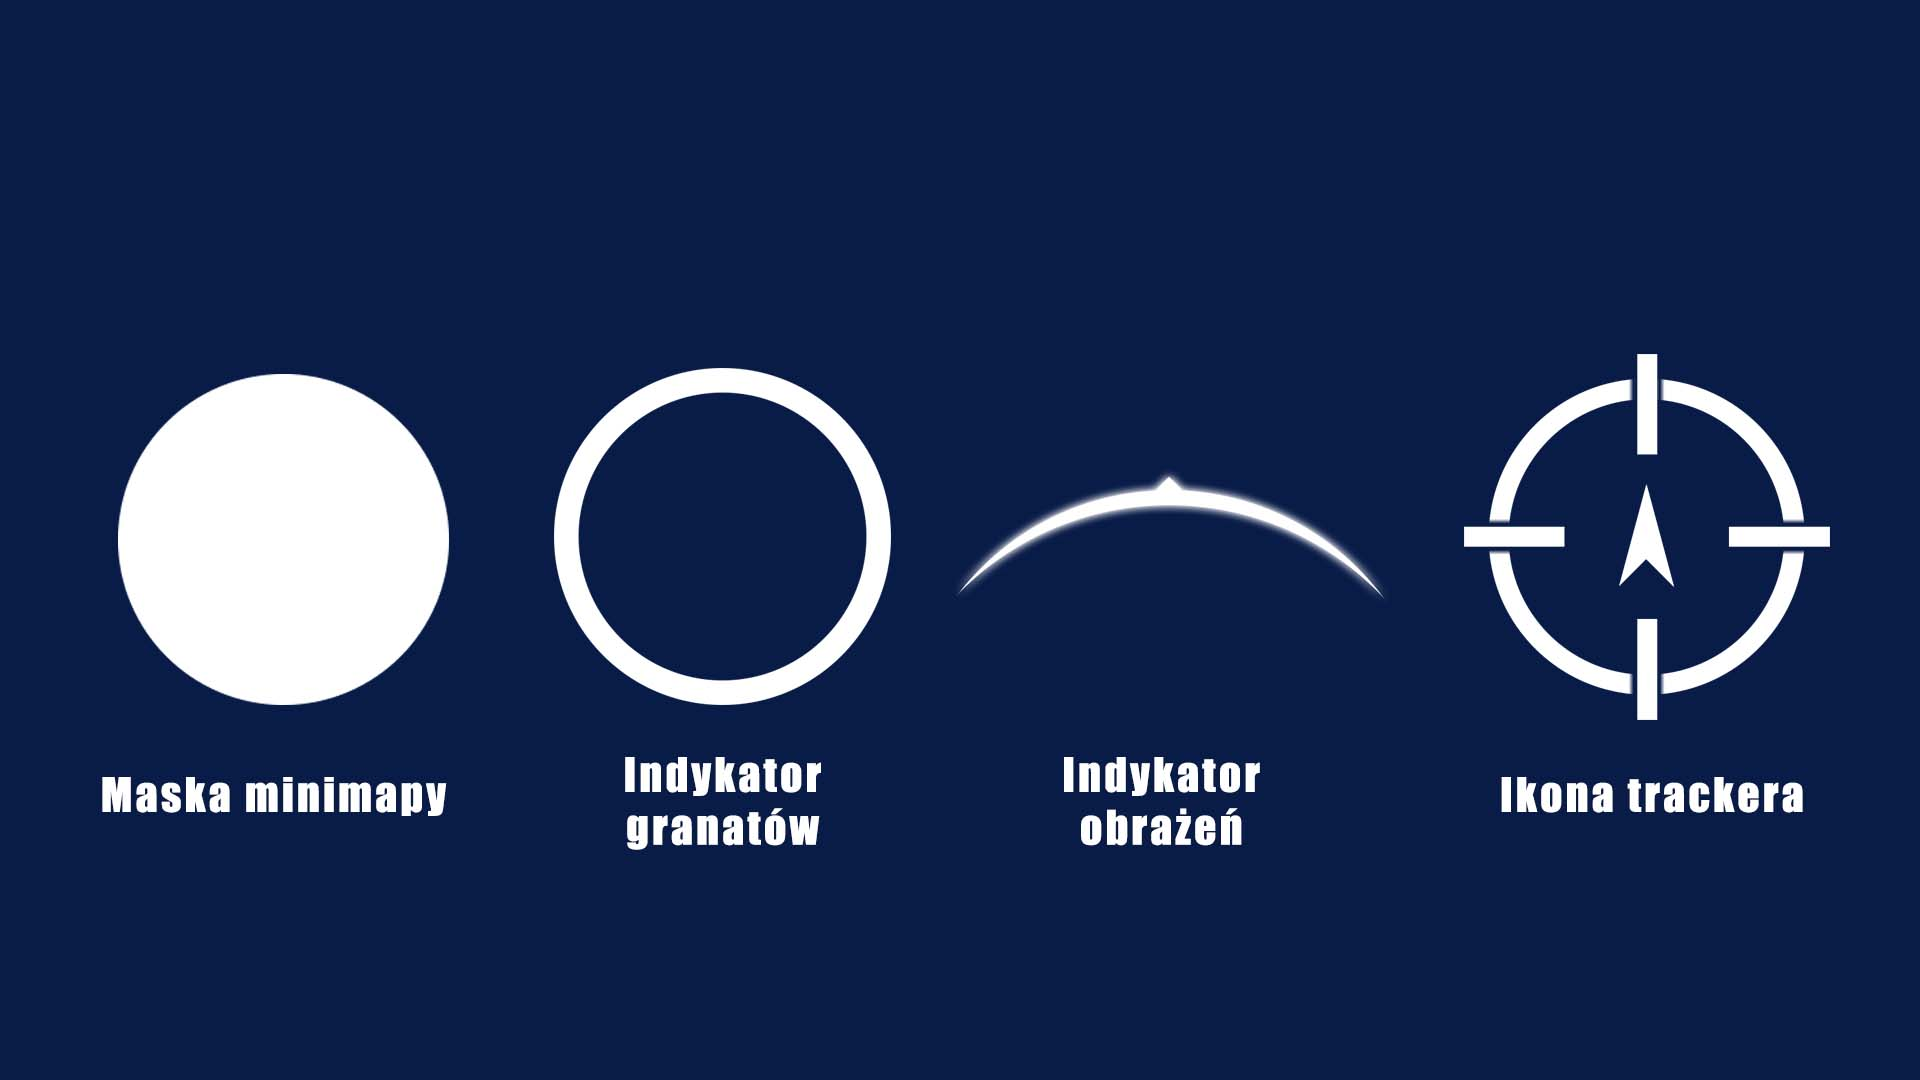
\includegraphics[scale=0.2]{Images/Pokazaniegranatow.jpg}
    \caption{Plansza przedstawiająca wszystkie ikony broni oraz granatów w grze}
    \label{fig:visBuglist}
\end{figure}
\newpage
\subsection{Integracja grafiki z interfejsem}
Integracja grafiki z interfejsem w Unity 3D obejmuje proces łączenia elementów wizualnych, takich jak obrazy, tekstury, czy modele 3D, z interfejsem użytkownika (UI) gry. Poniżej przedstawiam ogólny opis tego procesu:

\begin{enumerate}
  \item  \textbf{Utworzenie Interfejsu Użytkownika (UI):} Zacznij od stworzenia elementów interfejsu użytkownika, takich jak przyciski, teksty, obrazy, paski postępu, itp. W Unity, możesz użyć narzędzi dostępnych w systemie UI, takich jak Canvas, Image, Text itp.
  
  \item \textbf{Import Grafiki:} Przygotuj grafiki, które chcesz zintegrować z interfejsem. To mogą być pliki PNG, JPEG, czy inne formaty obsługiwane przez Unity. Importuj je do projektu Unity i umieść w odpowiednich folderach.
  
  \item \textbf{Umieszczanie Grafiki na Canvasie:} Przeciągnij i upuść grafiki na odpowiednie elementy UI, takie jak Image dla obrazków, czy Text dla tekstów. Upewnij się, że elementy graficzne są odpowiednio umieszczone na Canvasie, aby skonfigurować układ interfejsu.
  
  \item \textbf{Konfiguracja Grafiki w Edytorze:} W Edytorze Unity możesz dostosowywać właściwości grafik, takie jak rozmiar, kolor, przezroczystość, czy inne parametry. Edytor dostarcza intuicyjne narzędzia do manipulowania grafikami bez konieczności korzystania z zewnętrznych programów graficznych.
  
  \item \textbf{Animacje i Efekty Specjalne:} Jeśli chcesz dodać animacje lub efekty specjalne do grafik w interfejsie, możesz korzystać z komponentu Animator lub użyć skryptów w języku programowania obsługiwanym przez Unity, takim jak C\#.
  
  \item \textbf{Dostosowanie Interakcji:} Jeśli interakcje z elementami graficznymi mają być obsługiwane przez skrypty, napisz odpowiednie skrypty, aby reagować na interakcje gracza, takie jak kliknięcia myszą czy dotknięcia na ekranie dotykowym.
  
  \item \textbf{Testowanie na Różnych Rozdzielczościach:} Przetestuj interfejs na różnych rozdzielczościach, aby upewnić się, że elementy graficzne skalują się poprawnie i są czytelne na różnych urządzeniach.
  
  \item \textbf{Optymalizacja:} Dostosuj grafiki pod kątem optymalizacji, aby zoptymalizować wydajność gry, zwłaszcza jeśli planujesz publikację na różnych platformach.

\end{enumerate}

Integracja grafiki z interfejsem w Unity wymaga uwzględnienia aspektów wizualnych, funkcjonalności oraz dostosowania do potrzeb użytkownika, co pozwoli uzyskać atrakcyjny i skuteczny interfejs gry.

\newpage

\section{Animacje i efekty wizualne}\label{sec:anim}
W tym rozdziale zostaną omówione kluczowe aspekty związane z animacją postaci i obiektów w grze, specjalnymi efektami wizualnymi, oświetleniem oraz zastosowaniem shaderów z przykładami prostych shader graphów.
\subsection{System animacji postaci i obiektów}
W świecie gier komputerowych, animacje postaci oraz obiektów odgrywają kluczową rolę w kształtowaniu wrażeń gracza. Optymalne i realistyczne animacje są nieodzowne dla zapewnienia płynnej rozgrywki oraz ułatwienia zanurzenia się w wirtualnym środowisku. W tej sekcji omówione zostaną zaawansowane algorytmy stosowane do animowania postaci, takie jak Blend Trees, Inverse Kinematics (IK) oraz Ragdoll physics oraz animacje interaktywnych obiektów występujące w grze.


\subsubsection{Algorytmy wykorzystywane do animowania postaci}

\textbf{Blend Trees:} Technika Blend Trees jest wykorzystywana w animacjach postaci, umożliwiając płynne przejścia między różnymi animacjami w zależności od czynników takich jak ruch postaci, skok czy interakcje z otoczeniem. W grze jest stosowana dla osiągnięcia bardziej naturalnych i realistycznych animacji postaci.\\
\begin{figure}[h]
    \centering
    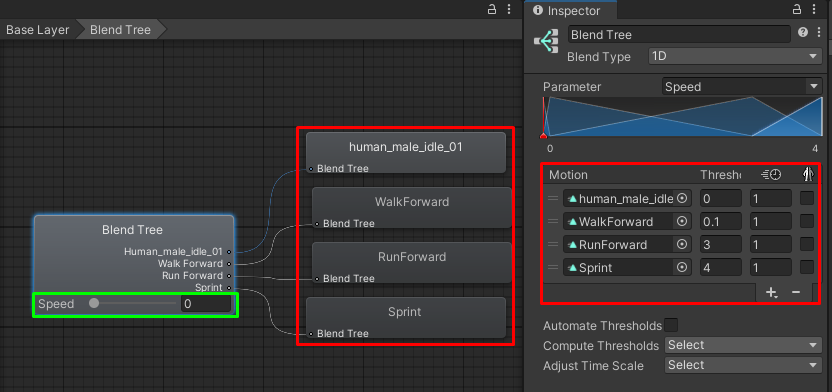
\includegraphics[width=1\linewidth]{Images/blendTree.png}
    \caption{Blend Tree dla płynnego przechodzenia między prędkościami poruszania dla AI}
\end{figure}
\FloatBarrier
\textbf{Inverse Kinematics (IK):}  Algorytm IK to technika matematyczna wykorzystywana w animacji komputerowej do określania pozycji stawów kości w celu osiągnięcia pożądanej pozycji końcowej. W grze IK jest używane do uzyskania bardziej realistycznych ruchów postaci poprzez dynamiczne dostosowywanie rotacji kości. Poniżej znajduje się fragment kodu (\textit{code snippet}), który wykorzystuje IK do dynamicznego dostosowywania rotacji określonych kości postaci przeciwnika, w celu precyzyjnego celowania w kierunku gracza:
\begin{codebox}
\begin{lstlisting}[language={[Sharp]C}, label={listing:WeaponIk.cs}]
public class WeaponIk : MonoBehaviour
{
    // ... (Remaining part of the script)

    private void LateUpdate()
    {
        if (aimTransform == null)
            return;
        if (targetTransform == null)
            return;

        Vector3 targetPosition = GetTargetPosition();

        for(int i = 0; i < iterations; i++)
            for(int j = 0; j < boneTransforms.Length; j++)
            {
                Transform bone = boneTransforms[j];
                float boneWeight = humanBones[j].weight * weight;
                AimAtTarget(bone, targetPosition, boneWeight);
            }
    }

    // ... (Remaining part of the script)
}
\end{lstlisting}
\end{codebox}
\captionof{lstlisting}{Klasa WeaponIk służąca do realistycznego symulowania ruchów kości podczas korzystania z broni przez AI}
\newpage
\textbf{Ragdoll physics:} Algorytm Ragdoll physics symuluje realistyczne reakcje postaci na siły zewnętrzne. W grze jest używany do nadawania postaci dynamicznych właściwości fizycznych po trafieniu lub upadku, co prowadzi do naturalnych animacji. W poniższym fragmencie skryptu odpowiadającym za fizykę ragdoll, zaimplementowano funkcje umożliwiające aktywację i dezaktywację ragdolla, co pozwala na dynamiczną zmianę zachowania postaci w zależności od sytuacji w grze. Dodatkowo, istnieje możliwość zastosowania sił zewnętrznych:
\begin{codebox}
\begin{lstlisting}[language={[Sharp]C}, label={listing:Ragdoll.cs}]
public class Ragdoll : MonoBehaviour
{
    // ... (Remaining part of the script)

    public void ActivateRagdoll()
    {
        foreach (var rigidBody in rigidBodies)
            rigidBody.isKinematic = false;

        if (animator != null)
            animator.enabled = false;
    }
    public void ApplyForce(Vector3 force)
    {
        var rigidBody = animator.
            GetBoneTransform(HumanBodyBones.Hips).
            GetComponent<Rigidbody>();
        rigidBody.AddForce(force, ForceMode.VelocityChange);
    }
}
\end{lstlisting}
\end{codebox}
\captionof{lstlisting}{Skrypt Ragdoll odpowiedzialny za symulowanie realistycznych reakcji postaci na siły zewnętrzne}
\newpage

\subsubsection{Animator przeciwników}
W tej sekcji przedstawiono użycie animatora przeciwników, gdzie wykorzystano warstwę broni wraz z zastosowaniem Avatar Mask. Avatar Mask został użyty do nadpisania animacji dla konkretnych części ciała przeciwnika. W tym przypadku zmienione zostało zachowanie głowy, tułowia oraz rąk podczas odtwarzania animacji na warstwie broni. Celem było zachowanie ruchu nóg z warstwy domyślnej do poruszania się, ale dostosowanie reszty kości do animacji wyciągania/trzymania/chowania broni.
\begin{figure}[h]
    \centering
    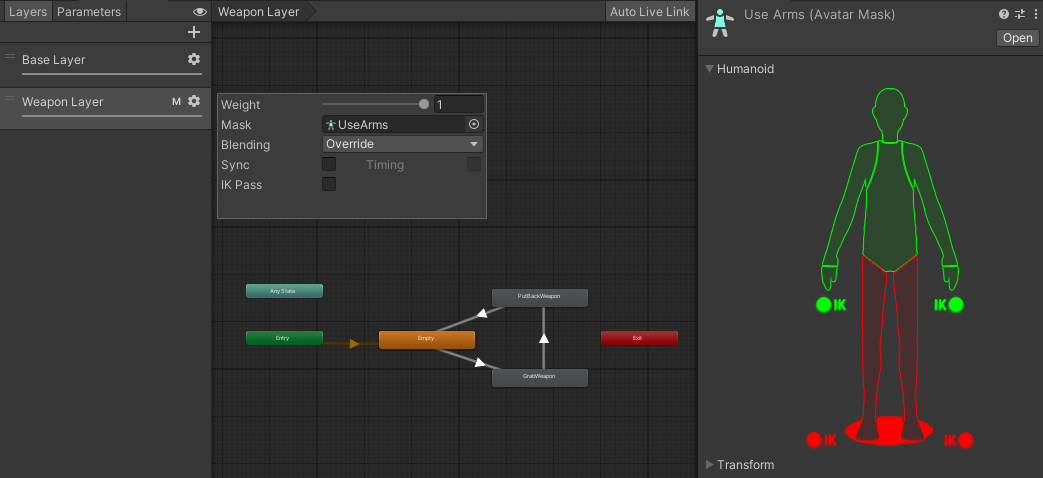
\includegraphics[width=1\linewidth]{Images/aiAnimatorController.png}
    \caption{Warstwa broni Animatora przeciwników i zastosowanie Avatar Maska}
\end{figure}

\subsubsection{Animator otwieralnych/zamykalnych obiektów}
W tej sekcji znajduje się animator otwieralnych i zamykanych obiektów, z ilustracją przykładowej skrzynki. W animatorze umieszczono dwie proste animacje: jedną z otwartą skrzynką, a drugą z zamkniętą. Zastosowano również parametr bool, który jest sterowany z poziomu kodu. Parametr ten działa na zasadzie toggla, co oznacza, że przy zmianie stanu otwiera lub zamyka skrzynkę, co skutkuje odtworzeniem odpowiedniej animacji.
\begin{figure}[h]
    \centering
    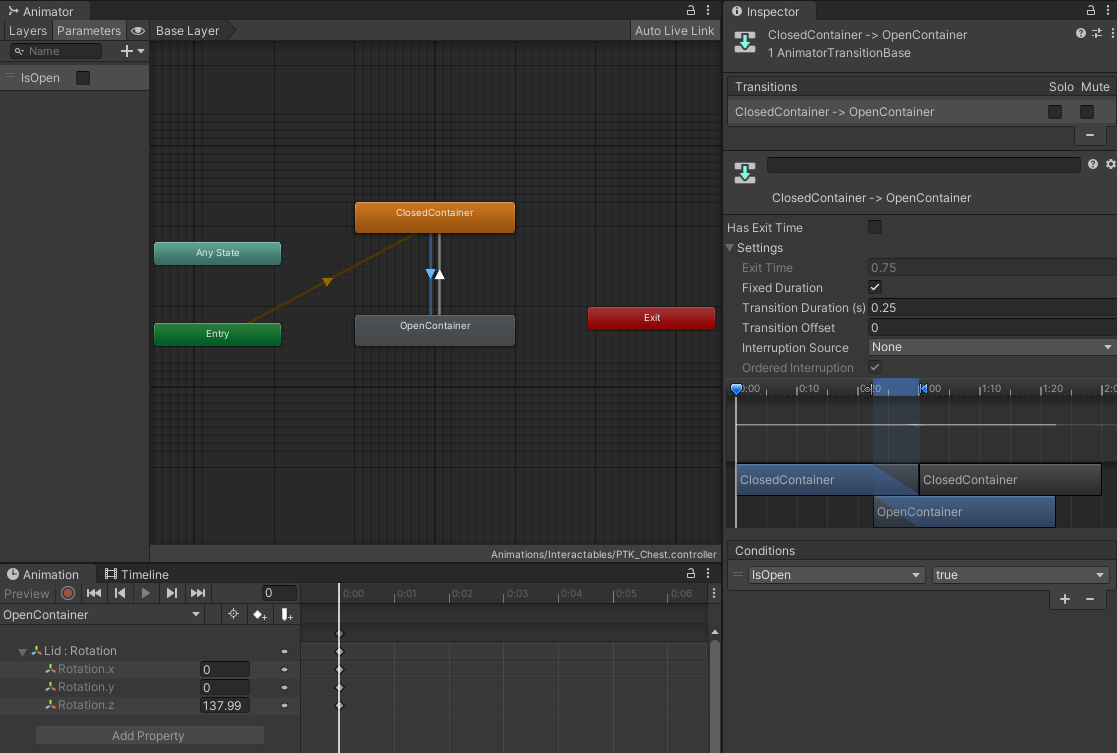
\includegraphics[scale=0.3]{Images/containerAnimator.png}
    \caption{Animator otwieralnego oraz zamykalnego obiektu na przykładzie skrzynki}
\end{figure}
\FloatBarrier
\subsection{Specjalne efekty wizualne}
W celu zwiększenia atrakcyjności wizualnej naszej rozgrywki zdecydowaliśmy się na wplecenie wielu elementów VFX czy systemów cząsteczkowych.
Ich wykorzystanie w znacznej części powiązane jest z mechanikami, takimi jak granaty:
\begin{itemize}
    \item Dymny - po wyrzuceniu go przez gracza następuje odliczanie, które po osiągnięciu wartości 0 wywołuje funkcje \textbf{ObjectPoolManager.SpawnObject}, która tworzy w miejscu granatu VFX dymu
    \item Podpalający (koktajl Mołotova) - po rozbiciu obiektu w jego miejscu pojawia się system cząsteczkowy, który wraca do puli obiektów po upływie czasu trwania oraz za pomocą VFX grafu nakłada na trafionych oponentów efekt podpalenia 
\end{itemize}

\subsubsection{Particle System}
Największym zauważalnym jego zastosowaniem jest otaczający obszar rozgrywki gaz.
Do jego stworzenia użyty została tekstura przykładowego gazu zaprezentowanego w paczce \textbf{"Particle Pack"} dostarczona przez Unity Technologies.
Sam Particle System posiada ograniczoną ilość generowanych cząsteczek (max 1000), został zapętlony by utrzymywał się podczas całej rozgrywki.
Ze względu na złożoność i sporą ilość rozmaitych ustawień w obrębie samego Particle Systemu, zdecydowanie łatwiej jest przedstawić konfigurację za pomocą zdjęć:
\begin{figure}[h]
    \centering
    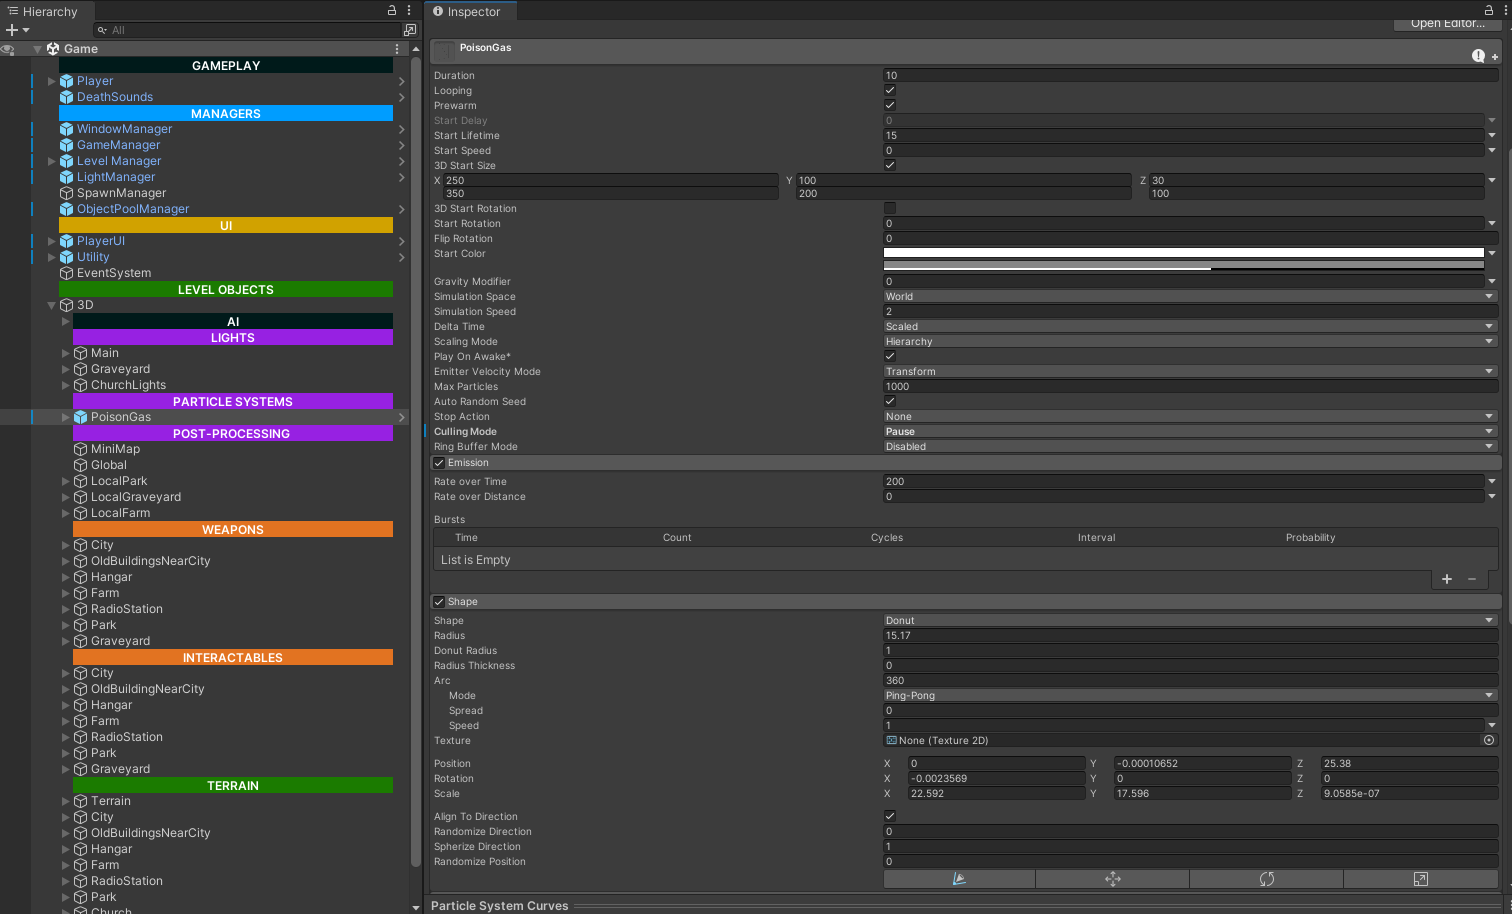
\includegraphics[width=1\linewidth]{Images/gaz1.PNG}
    \centering
    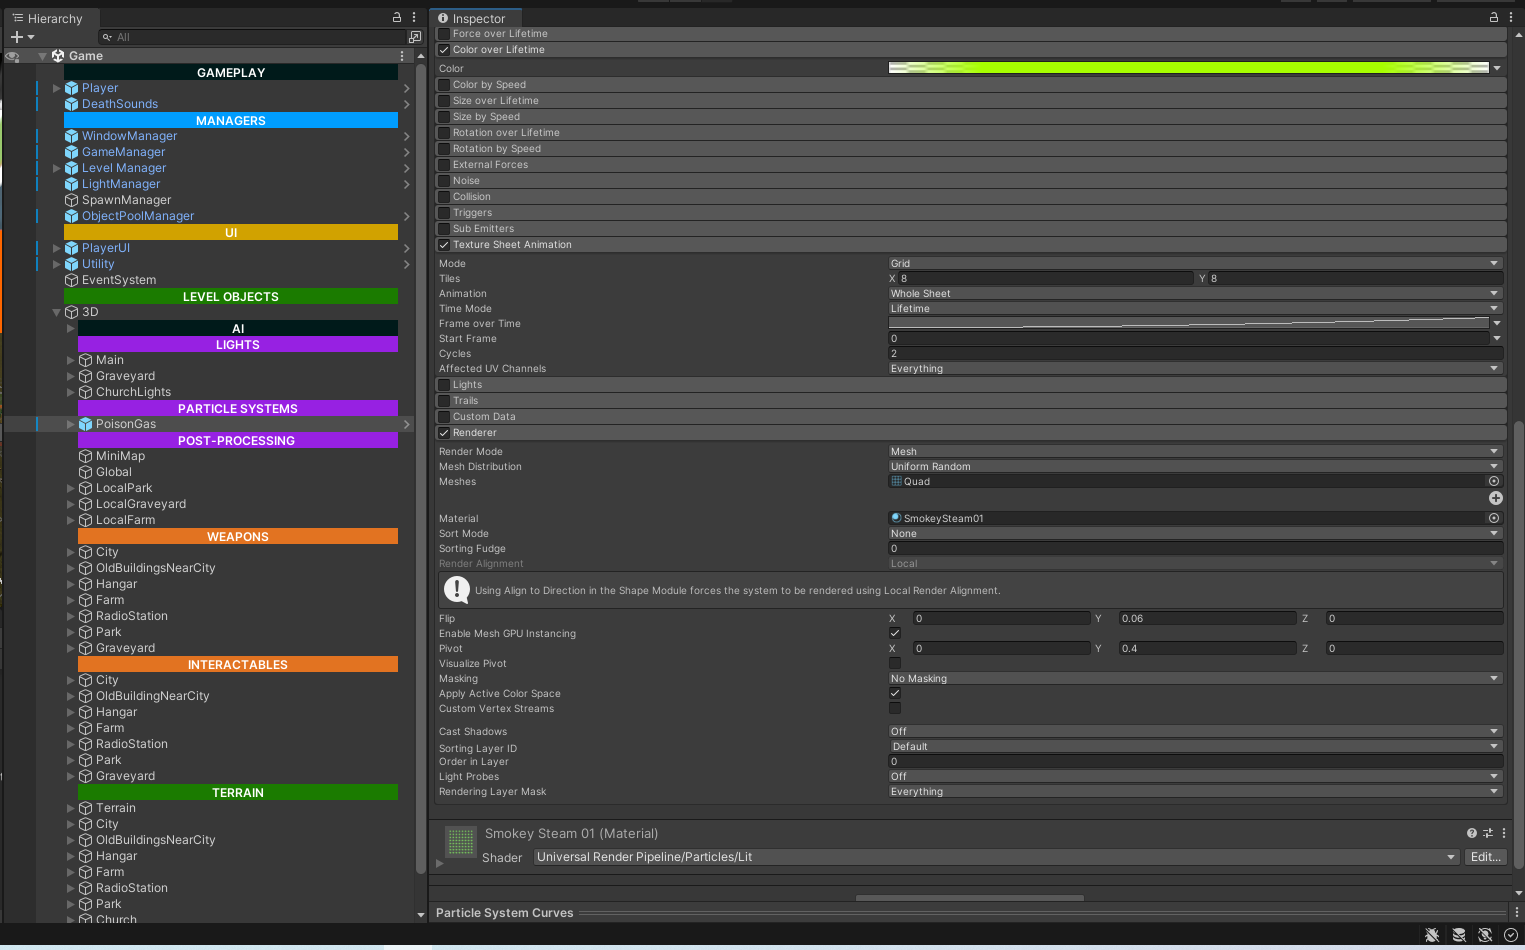
\includegraphics[width=1\linewidth]{Images/gaz2.PNG}
    \caption{Przedstawienie konfiguracji gazu}
\end{figure}
\FloatBarrier
\subsubsection{VFX}
\begin{itemize}
\item \texttt{Efekt podpalenia postaci:} Ten efekt pojawia się, gdy przeciwnik wejdzie w obszar pokryty ogniem z koktajlu Mołotowa. Postać staje się ognistą, co nie tylko wprowadza elementy wizualne, ale także może wpływać na mechanikę rozgrywki, dodając elementy takie jak obrażenia od ognia lub zmienione zachowanie postaci w płomieniach.
\begin{figure}[h]
    \centering
    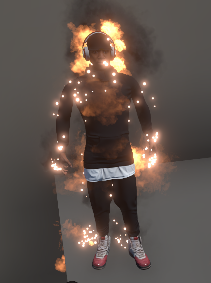
\includegraphics[scale=0.7]{Images/onFire.png}
    \caption{Efekt podpalenia w grze}
\end{figure}
\item \texttt{Efekt dymu:} Ten efekt aktywuje się w momencie użycia granatu dymnego. Tworzy gęsty dym, który może pełnić różne funkcje w grze, takie jak ukrywanie ruchów gracza przed przeciwnikami, zmiana taktyki lub tworzenie warunków do uniknięcia wykrycia. Jest to ważny element taktyczny wpływający zarówno na rozgrywkę, jak i na aspekty wizualne.
\begin{figure}[h]
    \centering
    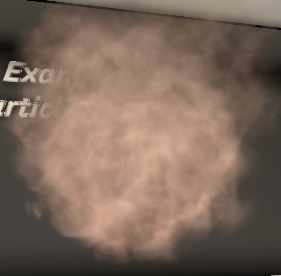
\includegraphics[scale=0.7]{Images/smoke.png}
    \caption{Efekt dymu w grze}
\end{figure}
\FloatBarrier
\end{itemize}
\subsection{Oświetlenie}
Oświetlenie odgrywa kluczową rolę w tworzeniu atmosfery i nastroju w grze. W naszym projekcie skupiamy się na zróżnicowanym wykorzystaniu oświetlenia, dostosowanym do różnych lokacji i sytuacji. Duża ilość oświetlenia znajduje się np. na cmentarzu, gdzie atmosfera musi być odpowiednio tajemnicza i klimatyczna.

\subsubsection{Dynamiczne oświetlenie}
Dynamiczne oświetlenie zostało zastosowane w głównej scenie gry w celu symulacji zmiany cyklu dnia i nocy. Szczególnie wykorzystane do tworzenia efektu realistycznego oświetlenia w różnych momentach rozgrywki. Więcej informacji na temat oświetlenia dynamicznego oraz jego wpływu na atmosferę gry można znaleźć w sekcji \nameref{subsubsec:skybox}.

\subsubsection{Wypieczone oświetlenie}
Wypieczone oświetlenie jest używane dla świateł, które nie wymagają dynamicznej zmiany w czasie rzeczywistym, co zdecydowanie poprawia optymalizację gry. Proces ten, znany jako wypiekanie świateł, pozwala na wcześniejsze przygotowanie oświetlenia dla statycznych scen, co przyczynia się do wydajniejszego renderowania. Aby dowiedzieć się więcej o wypiekanym oświetleniu, zobacz sekcję \nameref{subsubsec:bakingLights}.
\subsection{Zastosowanie shaderów}
W projekcie wykorzystano szereg zaawansowanych shaderów, które mają istotny wpływ na wizualną i atmosferyczną stronę gry. Poniżej znajdują się przykłady kilku zastosowanych shaderów. Warto zauważyć, że są to jedynie podstawowe i najprostsze przykłady użycia shaderów w naszym projekcie, ale używamy również bardziej skomplikowanych (np. do stworzenia okręgu z możliwością wyboru jego koloru czy ilości i odstępów jego segmentów lub do stworzenia fali, która porusza się po otaczającym nas terenie i ma za zadanie prezentować wizualnie wykorzystanie w grze trackera). \\ \\
\begin{figure}[h]
\textbf{Przykładowe Shadery:}
    \centering
    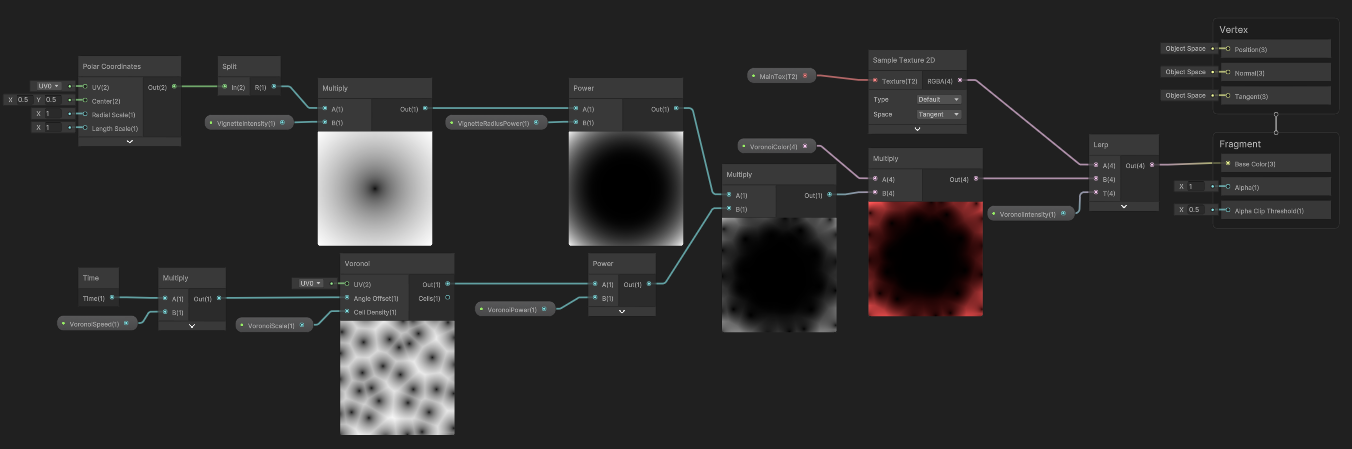
\includegraphics[width=1\linewidth]{Images/vignetteShader.png}
    \caption{Shader winiety odpowiedzialnej za wyświetlanie na ekranie gracza informacji o ilości utraconego życia}
\end{figure}
\begin{figure}[h]
    \centering
    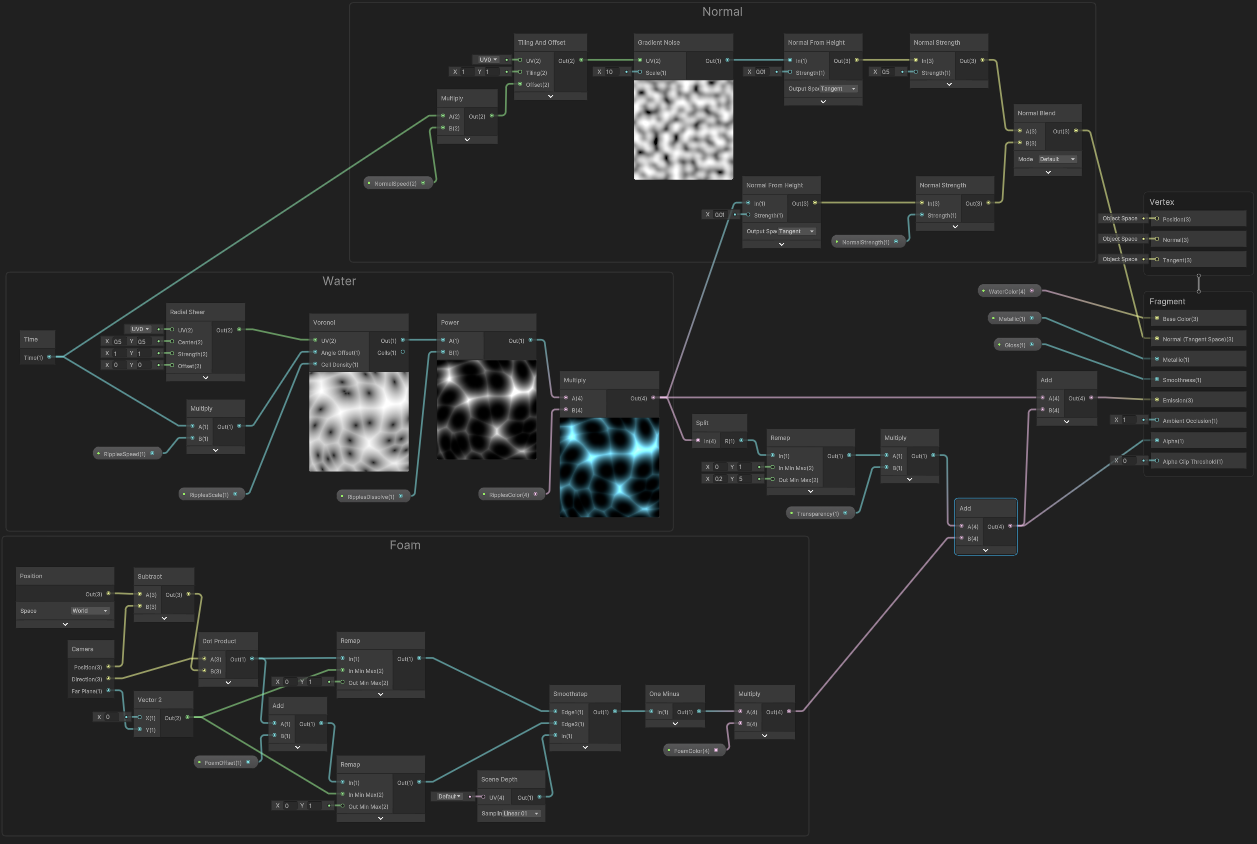
\includegraphics[width=1\linewidth]{Images/waterShader.png}
    \caption{Shader wody, którą znajdziemy w fontannie znajdującej się na terenie parku}   
\end{figure}
\begin{figure}[h]
    \centering
    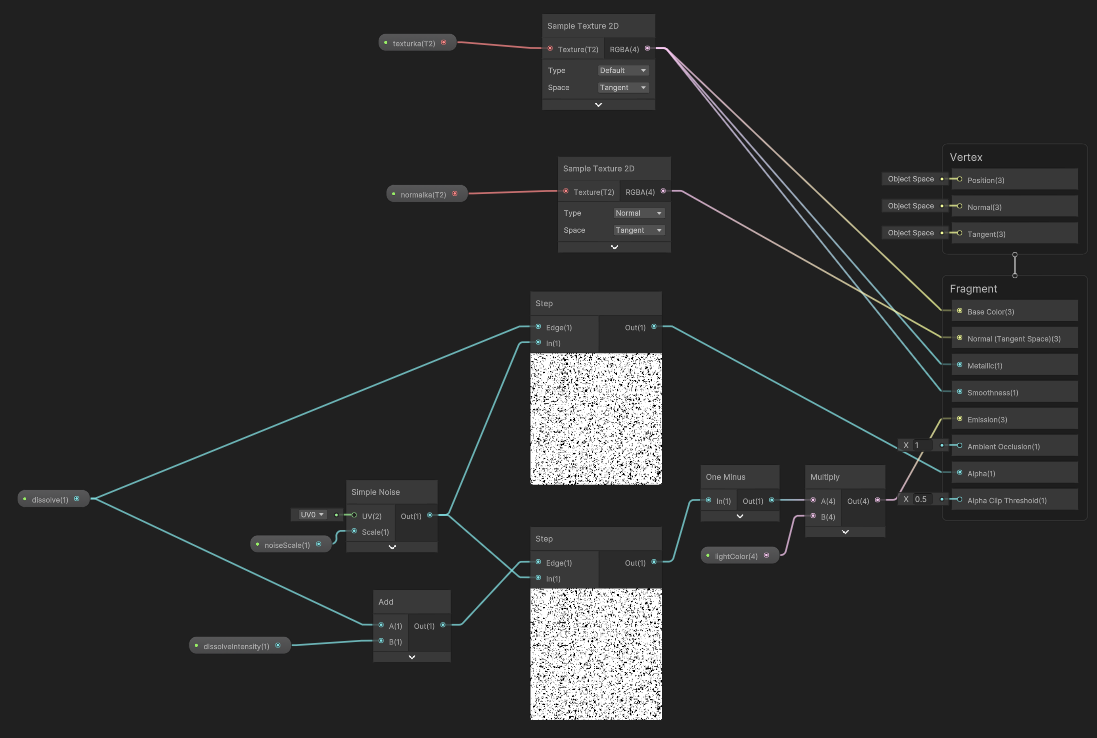
\includegraphics[width=1\linewidth]{Images/dissolve.png}
    \caption{Prostsza wersja shadera zanikania, używana w przypadku podniesienia interaktywnych obiektów takich jak kamizelka kuloodporna, apteczka czy granaty}
\end{figure}
\FloatBarrier

\newpage

\section{Poziomy (Level design)}\label{sec:leveldes}
Rozdział poświęcony poziomom stanowi kluczową część procesu tworzenia gier komputerowych, wpływając na doświadczenie gracza, narrację gry oraz ogólny poziom zabawy. W tym rozdziale omówione zostaną fundamentalne aspekty związane z projektowaniem poziomów.
\subsection{Planowanie i projektowanie poziomów}
Przed rozpoczęciem prac nad poziomem w celu uniknięcia konieczności poprawek  oraz gruntownych przebudów poziomu został sporządzony plan poziomu, który po dyskusjach w obrębie zespołu został zaakceptowany oraz wdrożony.
\\W trakcie planowania poziomu zostały przedyskutowane oraz uwzględnione następujące zagadnienia
\begin{itemize}
    \item \textbf{Tematyka poziomu w powiązaniu z założeniami gry} - jaki poziom pasuje do założeń naszej gry?
    Gdzie się znajduje? Jak fabuła tłumaczy wybór owego miejsca i w drugą stronę - w jaki sposób dobór lokacji i historia opowiadana przez miejsce wiąże się z naszą fabułą i ubogaca ją? Wybór padł na specjalnie odizolowane za pomocą gazu
    opuszczone miasto oraz okoliczną farmę i cmentarz. Głębsza analiza wyboru znajduje się tutaj:
    \nameref{est:story}
    \item \textbf{Cele poziomu} - jakich doświadczeń ma on dostarczyć graczowi? Jakie są warunki zwycięstwa? Czy celem jest stworzenie otwartego świata i pozwolenie graczowi na eksploracje - czy raczej należy stworzyć poziom liniowy, w którym gracz ma za zadanie dostać się z punktu A do punktu B - i jest on prowadzony w łatwy sposób?
    \item \textbf{Historia opowiadana przez poziom} - czy chcemy by nasz poziom opowiadał sobą historię - czy raczej chcemy ją graczowi przedstawić w inny sposób, a sam poziom ma być tylko planszą do rozgrywki.
    \item \textbf{Inspiracje i odniesienia} - czy już istnieją poziomy o podobnej tematyce lub założeniach?
    Jeżeli tak - to czy były dobre/złe? Jakie były ich mocne i słabe strony - oraz jak możemy uniknąć popełniania błędów innych ?
\end{itemize}
Po przeanalizowaniu powyższych pytań powstał pierwszy zamysł poziomu. W pierwotnych założeniach miał on ograniczać się do zamkniętego miasta, które po spełnieniu celu - pokonania wszystkich przeciwników - przekierowywałoby gracza do kolejnego poziomu - cmentarza.
\\ Następnie z cmentarza gracz po pokonaniu oponentów miał być kierowany do kolejnego, finałowego poziomu - lotniska.
Poziomy te w założeniach różniły się ilością przeciwników oraz dostępnym broniami.
\\Jednakże dalsza analiza potencjalnych plusów oraz minusów tego rozwiązania oraz porównanie z innymi grami podobnego gatunku doprowadziły do następujących wniosków:\\ \\
    \begin{itemize}
        \item Taki ciąg poziomów nie jest w żaden sposób uzasadniony fabularnie
        \item Liniowość tego rozwiązania negatywnie wpływałaby na satysfakcje graczy
        \item Gry z gatunku battle-royal uniwersalnie stosują jeden, rozległy poziom, podzielony na pomniejsze lokacje.
    \end{itemize}
W związku z powyższymi wnioskami końcowy koncept uległ zmianie i zamiast trzech odrębnych poziomów, użyty został koncept jednego, większego poziomu, który zawiera w sobie powyższe lokacje.
Dodatkowo, lotnisko będące planowanym ostatecznym poziomem, zostało zamienione na farmę.
Decyzja ta uzasadniona była wielkością lokacje oraz prędkością poruszania się gracza - w skali świata lokacja ta zaburzałaby proporcje pomniejszych lokacji jak również nadmiernie spowalniałaby tempo rozgrywki.

    

\subsection{Implementacja interakcji w środowisku}
\subsubsection{Rodzaje przedmiotów do interakcji}
Ze względu na charakterystykę gatunku gry, główną częścią interaktywnych obiektów stanowią bronie.
Zaimplementowane w grze zostało 5 broni (2 z nich występują w różnych wariantach kolorystycznych):
\begin{itemize}
    \item Pistolet (warianty czarny, biały, brązowy)
    \item Rewolwer
    \item Strzelba
    \item Karabin (warianty jak pistolet)
    \item Karabin Sniperski
\end{itemize}

Wprowadzone zostały również obiekty powiązane z mechanikami w grze:
\begin{itemize}
    \item Apteczka - w celu uzupełniania punktów zdrowia - występują obecnie dwa warianty - bazujące na takim samym meshu, lecz używające innej tekstury
    \begin{enumerate}
        \item Czarna - odnawia 15 \% maksymalnych punktów zdrowia
        \item Czerwona - odnawia 35 \% maksymalnych punktów zdrowia
    \end{enumerate}
    \item Skrzynka z amunicją - po wejściu w interakcje sprawdza ilość amunicji gracza, jeżeli jest ona różna od maksymalnej (przez maksymalną rozumie się trzykrotność pojemności magazynka) dla dowolnej z broni noszonej przez gracza - pozwala na uzupełnienie amunicji do ilości maksymalnej
    \item Pancerz - po wejściu w interakcje sprawdza obecną wartość pancerza gracza - jeżeli jest różna od 100\%, uzupełnia ją do maximum
    \item Gaz - interakcja odbywa się nie jak w wszystkich powyższych - przez odpowiedni klawisz - lecz przez wejście gracza w zakres collidera. \\
    Wejście w zakres collidera odpala funkcje zadającą bohaterowi obrażenia w czasie.
    \item Szkło - została zaimplementowana możliwość rozbijania obiektów.//
    Żeby tego dokonać, za pomocą kodu obiekt szkła sprawdza za pomocą collidera kolizje z pociskami wystrzelonymi przez gracza/bota.\\
    W momencie wykrycia takowej kolizji następuje eksplozja niszcząca szkło oraz podmiana prefabu na odłamki szkła.\\
    Otwiera to szerokie spektrum możliwości w kontekście tworzenia poziomu - bowiem znieczenie takowego szkła posiada równiez towarzyszący temu dźwięk - co może informować gracza o obecności przeciwników.
    Dodatkowo, otwiera to możliwość strzelania przezz przestrenie które nie sa blokowane szkłem po zniszczeniu go.
    \item Skrzynie z granatami - zasada działania jest podobna do skrzyni z amunicją ( tutaj maksimum dla danego typu granatu wynosi 3) - jednak sprawdza ona wszystkie z 3 możliwych typów granatów
    \begin{enumerate}
        \item Wybuchowy - warto wspomnieć że on również jest w stanie wchodzić w interakcje z szkłem tj. niszczyć
        \item Dymny - po rzuceniu triggeruje się Particle Effect, tworzący dym na małym obszarze
        \item Hukowo-błyskowy - po rzuceniu, wybucha, w momencie kiedy gracz patrzy w kierunku granatu w momencie, na ekranie zostaje wyświetlony biały canvas zasłaniający cały ekran, który wraz z czasem zanika (poprzez obniżanie jego alphy), dodatkowo wybuchowi towarzyszy głośny dźwięk
    \end{enumerate}
    \item Skrzynie\\\ trumny - wejście w interakcje triggeruje animacje otwarcia skrzyni (lub trumny), wewnątrz której można znaleźć broń (nie każda skrzynia zawiera broń, obiekty broni są dodawane ręcznie do owych skrzynek)
    \end{itemize}
Oprócz wyżej wymienionych elementów związanych z mechanikami, gracz może wejść również w interakcje z:
    \begin{itemize}
        \item drzwiami przesuwnymi - otwierają się w momencie wejścia w kolizje z colliderem gracza
        \item drabiną - podejście pozwala na wspinanie się gracza w celu uzyskania dostępu do wybranych lokacji
        \item bramą - wejście w interakcje otwiera ją, umożliwiając graczowi wejście na cmentarz
    \end{itemize}
\subsubsection{Sposób implementacji}
Wszystkie z powyższych interaktywnych obiektów zostały przygotowane jako prefaby, z podpiętymi wszystkimi niezbędnymi komponentami oraz skryptami \\
Następnie owe prefaby zostały wkomponowane w poziom, z uwzględnieniem balansu poprzez rozmieszczenie słabszych broni w łatwiej dostępnych lub bardziej oczywistych lokacjach, natomiast potężniejsze wyposażenie zostało ukryte w skrzyniach w cięższych do osiągnięcia lokacjach (przez trudność dostania się do lokacji rozumiane jest albo wyzwanie pod kątem zręcznościowym - wymaga skoków i odpowiedniego poruszania, lub spora ilość przeciwników w danej lokacji)
Wyjątkiem od wyżej wymienionej zasady jest gaz - który został użyty jako immersyjny sposób do ograniczenia wielkości poziomu.

\begin{figure}[h]
        \centering
        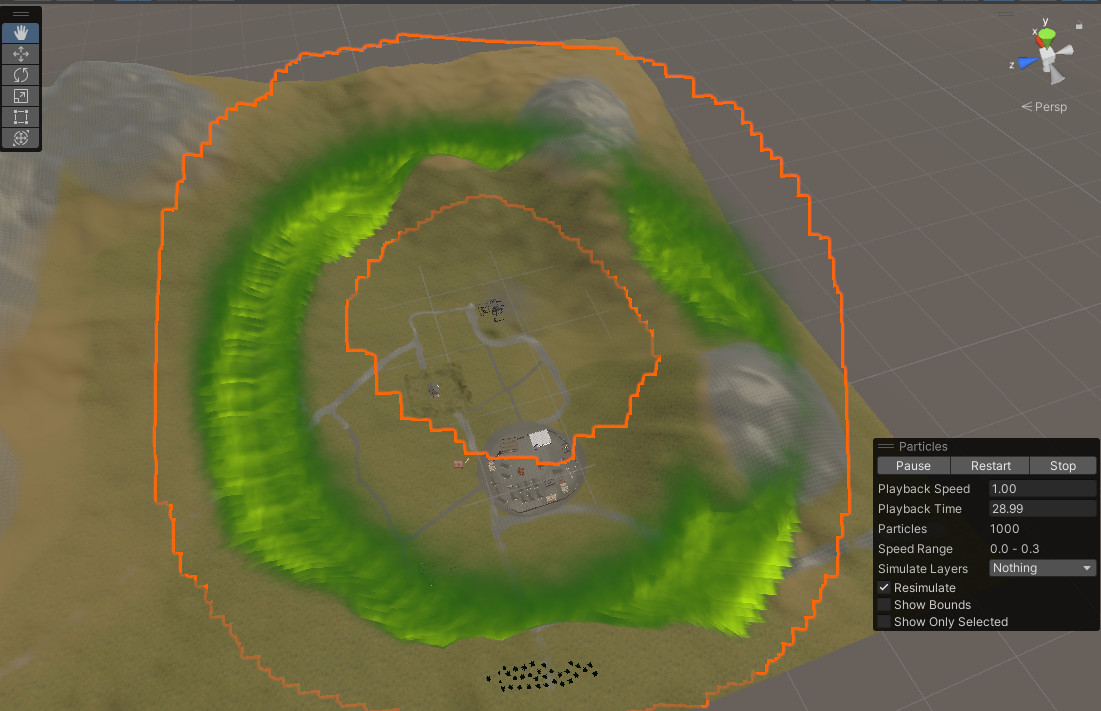
\includegraphics[width=1\linewidth]{Images/gas.png}
        \caption{Zastosowanie gazu jako naturalnego ograniczenia wielkości poziomu.}
        \label{fig:enter-label}
\end{figure}


\subsection{Rozkład przestrzeni}
\subsubsection{Struktura Ogólna Poziomu}
To tutaj kształtuje się świat gry, definiując główne obszary, trasy poruszania się gracza oraz punkty kluczowe. Zrozumienie tej struktury jest kluczowe dla zapewnienia płynności i logiczności rozgrywki. W tym kontekście, zajmiemy się analizą, jak zorganizować przestrzeń, aby stworzyć poziom, który nie tylko przyciąga wzrok, ale również dynamicznie reaguje na decyzje gracza.\\
W celu zapewnienia dynamiki naszemu poziomowi, postawiliśmy na rozwiązanie pozwalające uniknąć nadmiernego wczytywania - czyli umieszczenie wszystkich segmentów poziomu - w obrębie jednej sceny Unity.
Dodatkowo zastosowanie asynchronicznego ładowania sceny pozwoliło na stworzenie dużego poziomu bez większych problemów pod kątem wydajności.\\
Rozwiązanie to ma jednak swoje ograniczenia - utrudnia wprowadzanie zmian w scenie więcej niż jednej osobie ze względu na sposób przechowywania danych na temat sceny w jednym pliku - więc potencjalne jednoczesne wprowadzania zmian może prowadzić do niemożliwości otwarcia sceny/problemów przy commitach.
Wszelkie obiekty umieszczone na scenie znajdują się w hierarchii sceny tutaj:\\
\begin{figure}[h!]
    \centering
    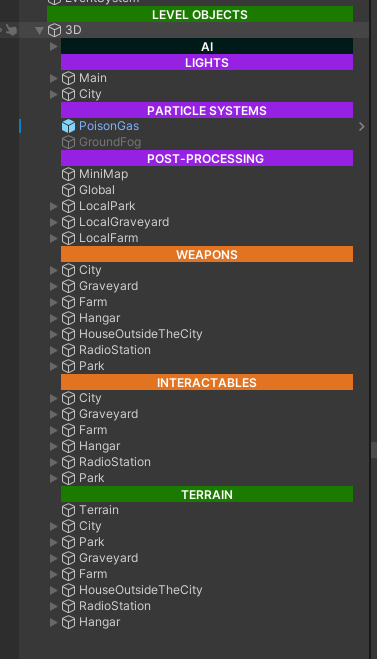
\includegraphics[width=0.41\linewidth]{Images/lvlhierarchy.png}
    \caption{Hierarchia obiektów na mapie}
    \label{fig:lvlhierarchy}
\end{figure}
\\Obiekty jak trawa, drzewa oraz kamienie dostępne są do edycji oraz rozmieszczania z poziomu ustawień terenu - to samo dotyczy wszelkich tekstur użytych do malowania podłoża:
\begin{figure}[h!]
    \centering
    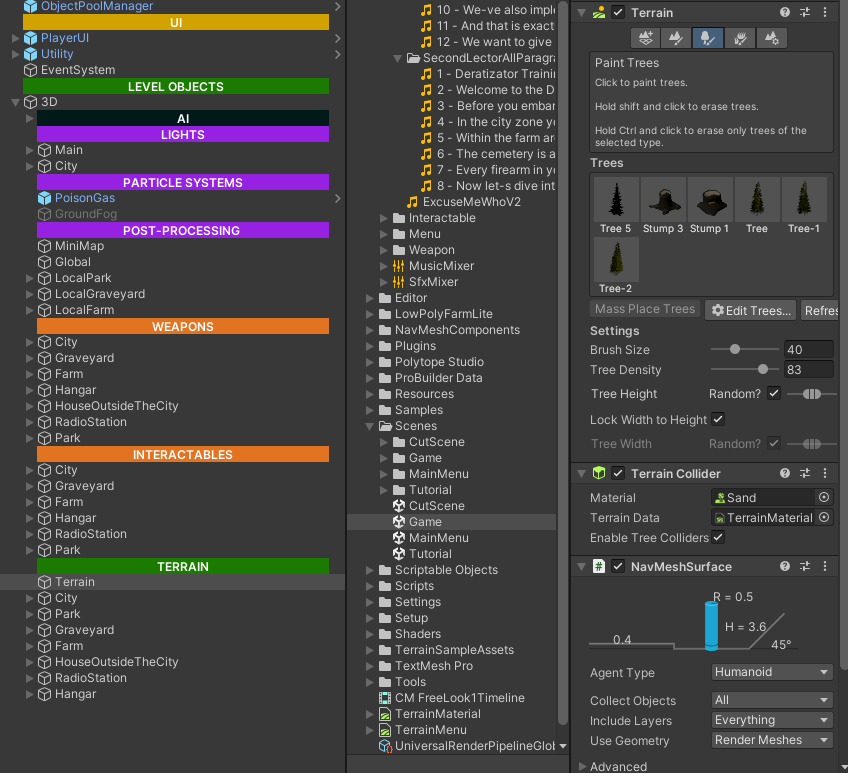
\includegraphics[width=0.65\linewidth]{Images/terrain.png}
    \caption{Ustawienia drzew na mapie - z poziomu terenu}
    \label{fig:enter-label}
\end{figure}
\begin{figure}[h!]
    \centering
    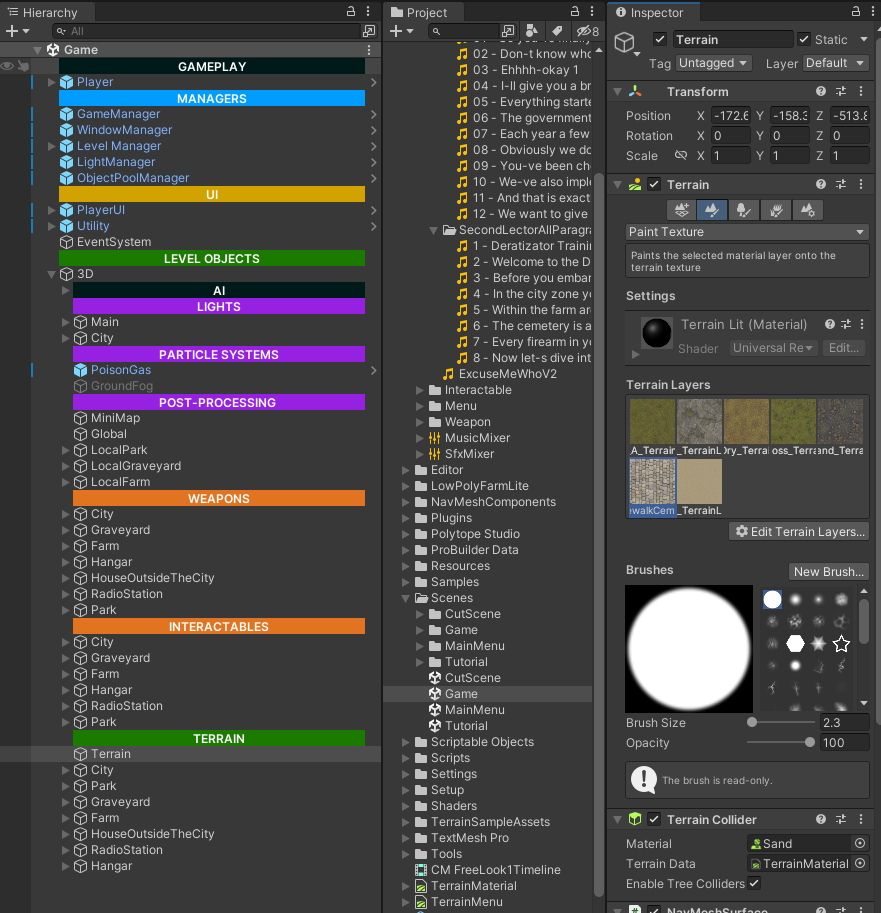
\includegraphics[width=0.65\linewidth]{Images/image.png}
    \caption{Użyte tekstury}
    \label{fig:enter-label}
\end{figure}
\newpage
\subsubsection{Sekcje i Obszary Kluczowe}
Poziom został podzielony na 4 główne sekcje, które wraz z postępami prac zostały rozdzielone na mniejsze obszary kluczowe.
Dodatkowo powstała również lokacja będąca łączeniem między sekcjami - w celu bardziej angażującej podróży pomiędzy owymi strefami - oraz makieta potencjalnej lokacji, która jednakże nie została wykorzystana - dostęp do niej jest zablokowany przez gaz - jednakże ze względu na aspekt wizualny (daje ona wrażenie że poza gazem również są tereny) została ona zachowana w obecnym scenariuszu
Strefy które możemy wyróżnić w grze to:
\begin{itemize}
    \item Cmentarz
    \item Miasto
    \item Farma
    \item Radiostacja
\end{itemize}
Wszystkie lokacje połączone są z sobą - dostep do nich jest nieograniczony - co daje graczowi dowolność w kolejności odwiedzania.

Wszystkie obiekty związane z danymi lokacjami są odpowiednio pogrupowane w celu ułatwienia nawigacji przy potencjalnym wprowadzaniu zmian:
\begin{figure}[h]
    \centering
    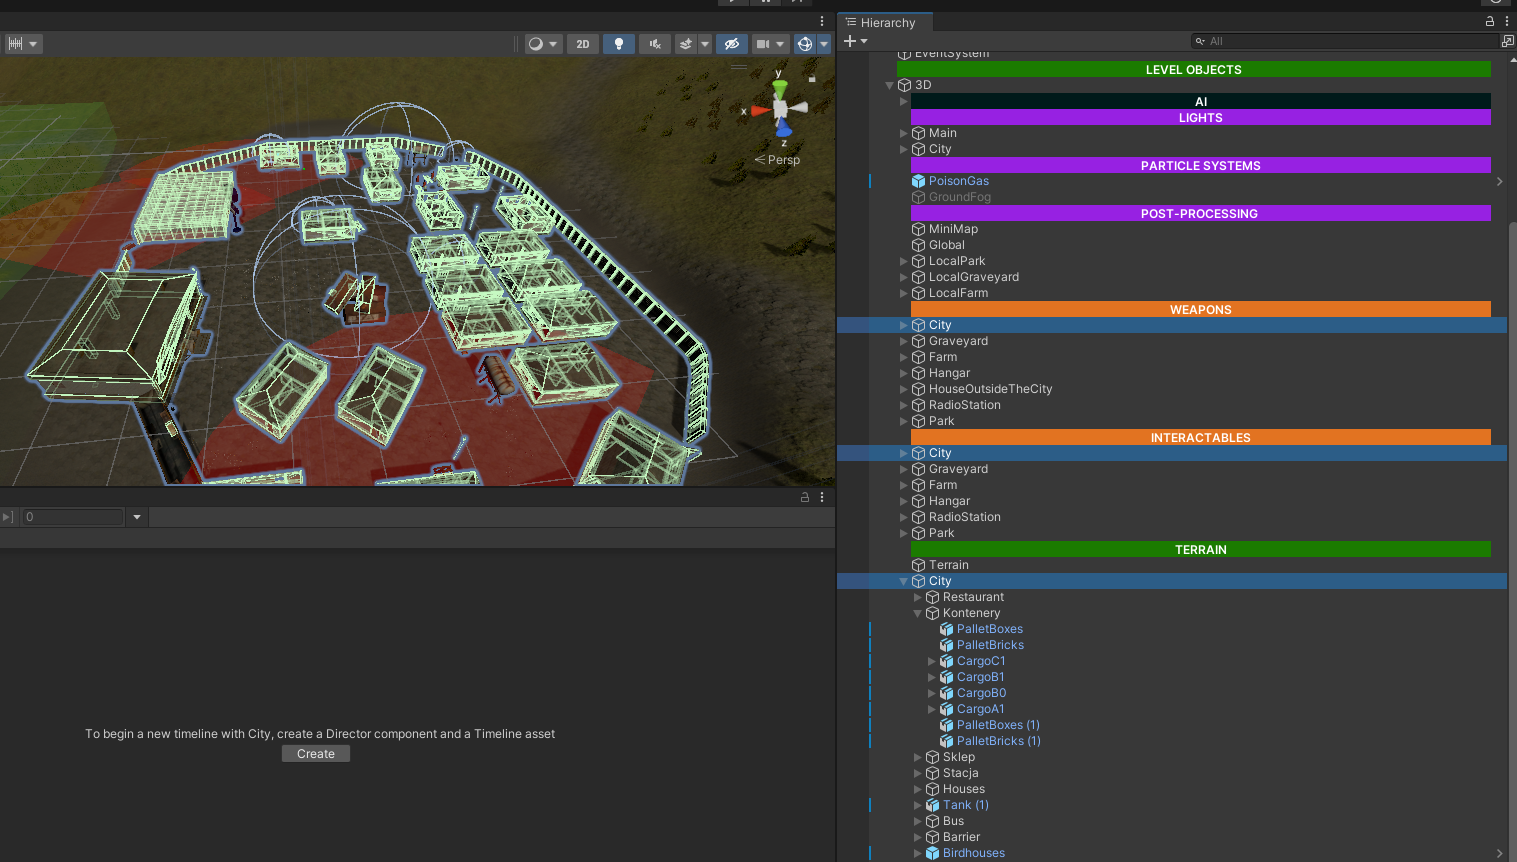
\includegraphics[width=1\linewidth]{Images/cityexamplehierarchy.png}
    \caption{Przykład hierarchii dla sekcji miasta}
    \label{fig:enter-label}
\end{figure}
Każda z sekcji jest również rozbita na obszary kluczowe dla niej - główne punkty uwagi gracza, które będą najczęściej odwiedzane
Są to:
\begin{itemize}
    \item Dla miasta są to:
    \begin{itemize}
        \item Restauracja
        \item Stos kontenerów na środku
        \item Wrak autobusu
        \item Sklep
        \item Sekcja domków szeregowych - 7 identycznych domów w rzędach
        \item Stacja benzynowa
    \end{itemize}
    \item Sekcja cmentarza jest podzielona na:
    \begin{itemize}
        \item Sekcja wejściowa- brama praz nagrobki
        \item Sekcja środkowa - ołtarz oraz kolumny
        \item Sekcja tylnia- kurhany, mniejszy wydzielony fragment z nagrobkami
    \end{itemize}
    \item Farma została podzielona na
    \begin{itemize}
        \item Sekcja domów
        \item Pola uprawne
    \end{itemize}
    \item Radiostacja posiada następujące punkty zainteresowania:
    \begin{itemize}
        \item Budynek Radiostacji
        \item Kontenery z skrzyniami
    \end{itemize}
\end{itemize}

Taki rozkład znacznie ułatwiał pracę nad poszczególnymi lokacjami - każdy z punktów kluczowych został osobno zaprojektowany i wdrożony, następnie połączenie ich dawało praktycznie gotową lokację.
\subsubsection{Połączenia Między Sekcjami}

Połączenia między sekcjami muszą być zarówno interesujące pod kątem posiadanej zawartości - jak również wizualnie.
Jednocześnie w dalszym ciągu powinny być łatwo widoczne oraz intuicyjne dla gracza.
Ze względu na rozmiar mapy  jak i zastosowanie minimapy intuicyjność wyboru ścieżki i miejsca dokąd prowadzi nie stanowi żadnego wyzwania pod kątem tworzenia poziomu - gdyż lokacje są widoczne.\\
W ramach zachęty do stosowania przez gracza wytyczonych ścieżek - pozostałe trasy posiadają dużą ilość drzew.
Powoduje to znaczne spowolnienie w przemierzaniu terenu - jednakże gwarantuje większą ochronę - gdyż drzewa posiadają collidery, co sprawia że pocisk wystrzelony w strone gracza może zatrzymać się na obiekcie drzewa.\\
Zastosowane w grze ściezki zostały wykonane przez naniesienie odpowiedniej, różnej od pozostałej powierzchni, tekstury - by za pomocą skojarzeń z dnia codziennego przekazać informacje "to jest ścieżka" graczowi.
\begin{figure}[h]
    \centering
    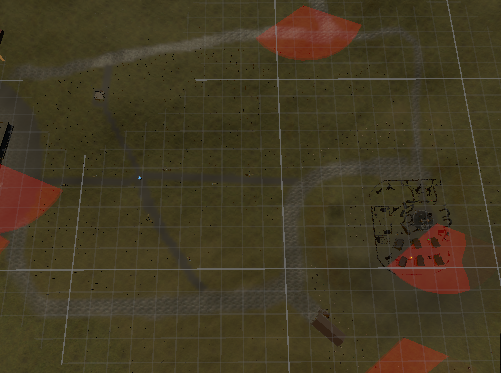
\includegraphics[width=0.5\linewidth]{Images/paths.png}
    \caption{Sciezki naniesione na teren za pomoca tekstury}
    \label{fig:enter-label}
\end{figure}

W celu urozmaicenia podróży gracza, na przecięciu najważniejszych ścieżek prowadzących do głównych sekcji wymienionych wyżej, została wprowadzona nowa podlokacja - Park.
Umieszczenie kilku ławek, koszy oraz latarnii z dodaną emisją sprawiło że ścieżka nie sprawia wrażenie pustej, świat wydaje się żywszy i realniejszy.
Dodatkowo gracz może znaleźć po drodze na kilka broni - co okazało się konieczne w sytuacjach gdzie AI w agresywny sposób wykorzystało dostępne na mapie zasoby i zmusiło gracza do ucieczki - pozwoliło to uniknąć sytuacji gdzie gracz ginie bez możliwości sensownej obrony.

Warto również wspomnieć że wszelkie lokalizacje mijane po drodze posiadają również teleportery, będace punktami startowymi dla gracza oraz botów. Poszczególne lokacje posiadają różne warianty kolorystyczne owych teleporterów, co może być swego rodzaju informacją dla gracza dzięki dobraniu kolorów powodującym skojarzenia:
\begin{itemize}
    \item Cmentarz \& kościół - pomarańczowy
    \item Radiostacja \& okolice - niebieski
    \item Farma - żółty
    \item Park\& okolice lasu między lokacjami - zielony
    \item Miasto - różowy
\end{itemize}
\subsection{Estetyka i atmosfera}\label{est:story}
Podział poziomu na pomniejsze sekcje doprowadził do decyzji zastosowania różnych estetyk dla poszczególnych lokacji.
Każda z nich posiada inną muzyke, zastosowane palety barw oraz assety czy oświetlenie.
Dzięki takiemu rozwiązaniu przemierzając poszczególne lokacje gracz w mniejszym stopniu odczuwa fakt że mapa jest zamkniętym wycinkiem - gdyż każda lokacja ma swoją historię którą graficznie przekazuje, i mogłaby stanowić osobny poziom.\\
Główne założenia odnośnie estetyki dla poszczególnych sekcji to:
\begin{itemize}
    \item Cmentarz - mroczna, ciężka, gotycka stylistyka, chłodne, ciemne barwy, odcienie czerni, szarości, miejscami rozświetlone przez pomarańczowe oświetlenie latarni oraz świec.
    Assety używające tekstur kamienia, grafitu, by jeszcze bardziej podkreślić mrok tego miejsca.
    Brak/minimalna roślinność, jeżeli występuje - to uschnięte krzewy, drzewa bez liści.
    Podłoże korzystające z tekstur odzwierciedlających suchą, uschniętą ziemie.
    Inspirowane scenami z filmów jak "Harry Potter i Czara Ognia" (sekwencja końcowa na cmentarzu), "Smętarz dla zwierzaków"
    \item Miasto - klimat znacznie lżejszy niż na cmentarzu, mimo to surowe miasto, wzorowane na miastach Europy wschodniej (wielka płyta).Miasto ma w założeniach sprawiać wrażenie opustoszałego - porozbijane szyby, zniszczone budynki, zardzewiałe wraki samochodów.
    Odcienie szarości i brązu, zastosowane materiały - beton, ciemne drewno, metale.
    Wyjątek - restuaracja - rozświetlona, jasna, nowoczesna, wydaje się nie pasować do pozostałych budynków.
    Brak roślinności.
    Podłoże - tekstura betonu.
    \item Farma - kontrast dla dwóch poprzednich lokacji, jasna, rozświetlona, sielankowo cukierkowa, ciepłe, żywe barwy, odcienie żółci i pomarańczu, kolory mocno nasycone, jaskrawe.
    Sporo roślinności, podłoże - jasna trawa
    Budynki drewniane, proste, wiejskie.
    \item Park - klimat letniego popołudnia, jako strefa środkowa mapy ma za zadanie wprowadzić pewien balans pomiędzy cmentarzem, a miastem tak aby gracz doświadczył w miarę płynnego przejścia klimatu pomiędzy lokacjami. 
    \item Radiostacja - położona na wzgórzu w okolicach parku z widokiem na całą mapę. Pełni po części funkcję punktu widokowego. Prosta drewniana konstrukcja z drobną piwniczką na sprzęt.
\end{itemize}


\subsection{Przerywniki filmowe}
\subsubsection{Rodzaje i zastosowanie  w grze cutscenek}
Po zebraniu feedbacku po playtestach część graczy zauważyła brak powiązania fabularnego między lokacją, do której trafia gracz a tytułem gry oraz stylistyką głównego menu.
Po przedyskutowaniu w obrębie zespołu postanowiliśmy stworzyć cutscenke wprowadzającą(intro), której zadaniem będzie stworzyc pomost między sceną na której znajduje się gracz, a tytułem.

Dodatkowo, postanowiliśmy również stworzyć odrębne cutscenki w ramach zakończenia rozgrywki (outro) - w dwóch wariantach,
w zależności czy gracz wygrał czy przegrał.
Z uwagi na decyzję o wdrozeniu również tutorialu w ramach cutscenki - polegającego na przeniesienie gracza na osobną scene. która wcześniej była używana do testowania nowych mechanik - a nastepnie możliwość przejścia z poziomu tutorialowego do gry głównej - implementacja into odbyło się na osobnej scenie z specjalnie przygotowanym środowiskiem którego przedstawienie znajduje się poniżej.
Takie rozwiązanie pozwoliło nam na zwiększenie ilości klatek na sekunde (FPS) podczas cutscenki - ze względu na brak konieczności renderowania oraz symulacji zachowania botów, pozbyciu się assetów broni, elementów interfejsu gracza, oraz samych mechanik powiązanych z graczem - takich jak poruszanie się, system ekwipunku, dynamiczna kamera (gracza jak i minimapy)

\subsubsection{Struktura sceny}
Do stworzenia scen outro - w obu wariantach - została wykorzystana scena \textbf{Game} - czyli scena główna na której odbywa się rozgrywka - ze względu na fakt że po zakończeniu rozgrywki, niezależnie od wygranej lub przegranej gracze - nic nie powstrzymuje nas przed usunięciem obiektów powiązanych z botami oraz graczem - oraz aktywowania obiektów stricte niezbędnych do scenki - gdyż rozgrywka sterowana przez gracza defacto dobiega końca.

Natomiast ze względu na wyżej opisane powody scena intro odbywa sie na specjalnie przygotowanej scenie \textbf{Cutscene}.
Jej struktura pod kątem obecnych obiektów rozbita została na 3 główne sekcje:
\begin{itemize}
    \item Lokacja 1 - dom - wykorzystane tutaj zostało identyczne ułożenie obiektów jak do menu głównego.
    \item Lokacja 2 - teren - jest to kopia terenu głównego rozgrywki - zmniejszona o nieużywane elementy powiązane z rozgrywką
    \item Obiekty związane z samą scenką - najszersza kategoria. znajdują się tutaj wszystkie kamery wraz z dollyCartami,
    warstwa UI odpowiedzialna za wyświetlanie napisów przy dialogach, wszelkie efekty wizualne oraz obiekty animowane na osi czasu.
    Dodatkowo w tej kategorii znajdziemy wszelkie Managery wykorzystane do zarzadzania przepływem pomiędzy scenami rozgrywki.
\end{itemize}

\subsubsection{Mechanizmy użyte w cutscence}
Rdzeniem naszych przerywników filmowych są trzy dostępne w samym Unity paczki - Cinemachine, Sequences oraz  Timeline.
Dodatkowo, bardzo ważną rolę odgrywa również paczka pozwalająca na sterowanie tekstami z TextMeshPro z poziomu timeline, stworzona przez Krisa Kreja.

Warto również wspomnieć o dubbingu, który został wygenerowany przy użyciu narzedzia \href{https://play.ht/}{AI text to speech}.
Poniżej screenshoty przedstawiające konkretne konfiguracje dla poszczególnych głosów:
\begin{figure}[h]
    \centering
    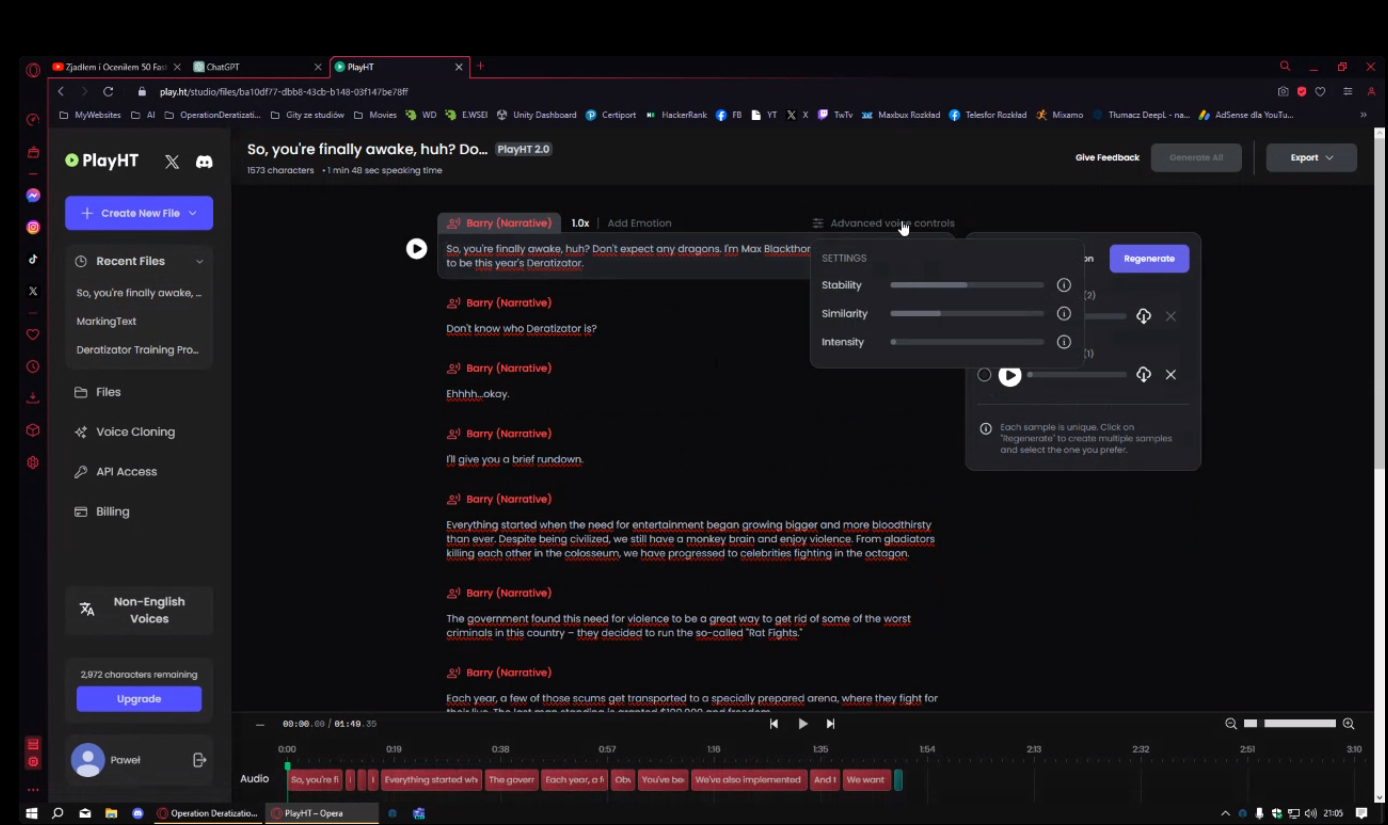
\includegraphics[width=0.5\linewidth]{Images/voice_max.PNG}
    \caption{Konfiguracja głosu dla Maxa - narratora pierwszej części intro}
    \label{fig:enter-label}
    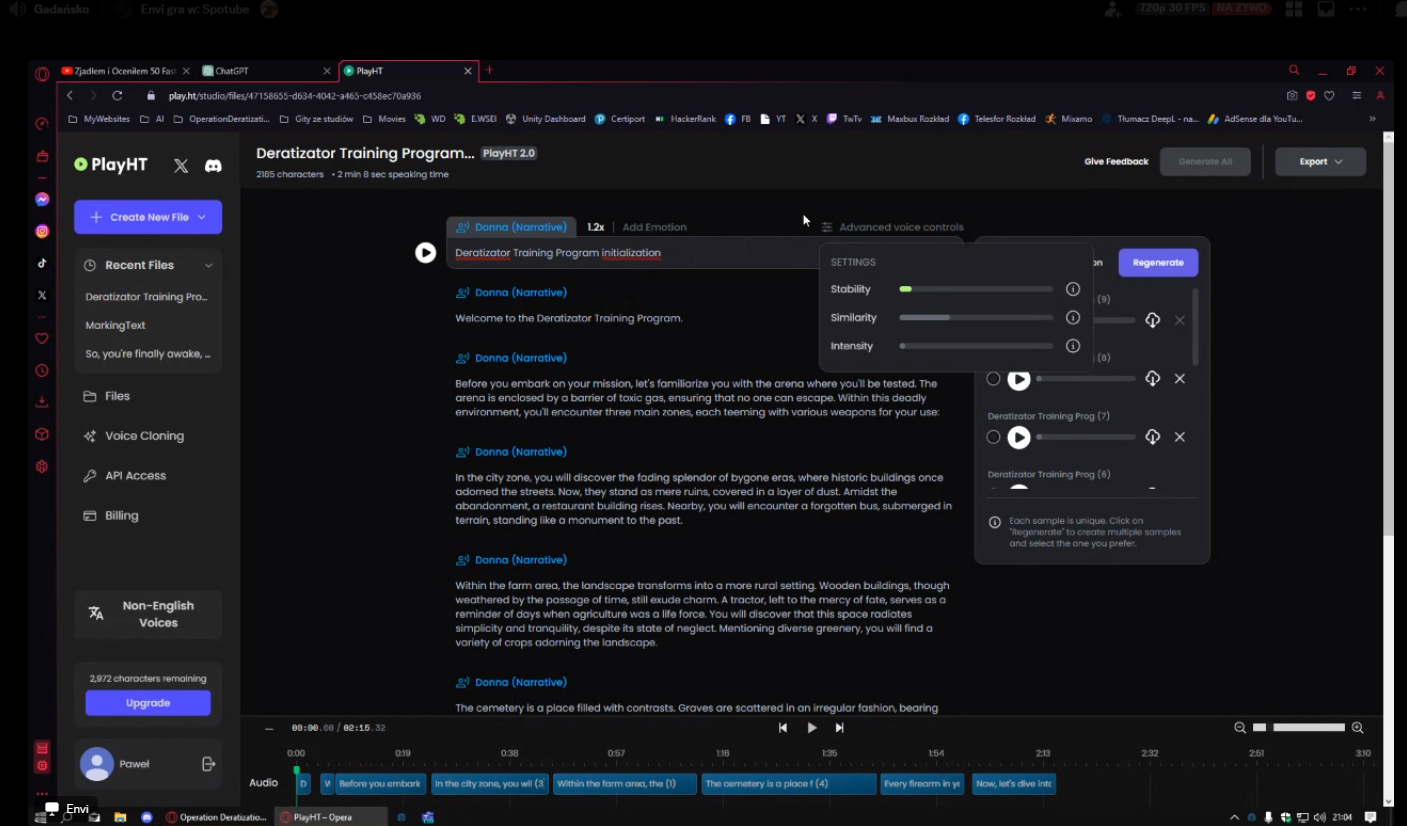
\includegraphics[width=0.5\linewidth]{Images/voice_intro_chip.png}
    \caption{Konfiguracja głosu dla narratora drugiej części intro - Smart Chip}
    \label{fig:enter-label}
    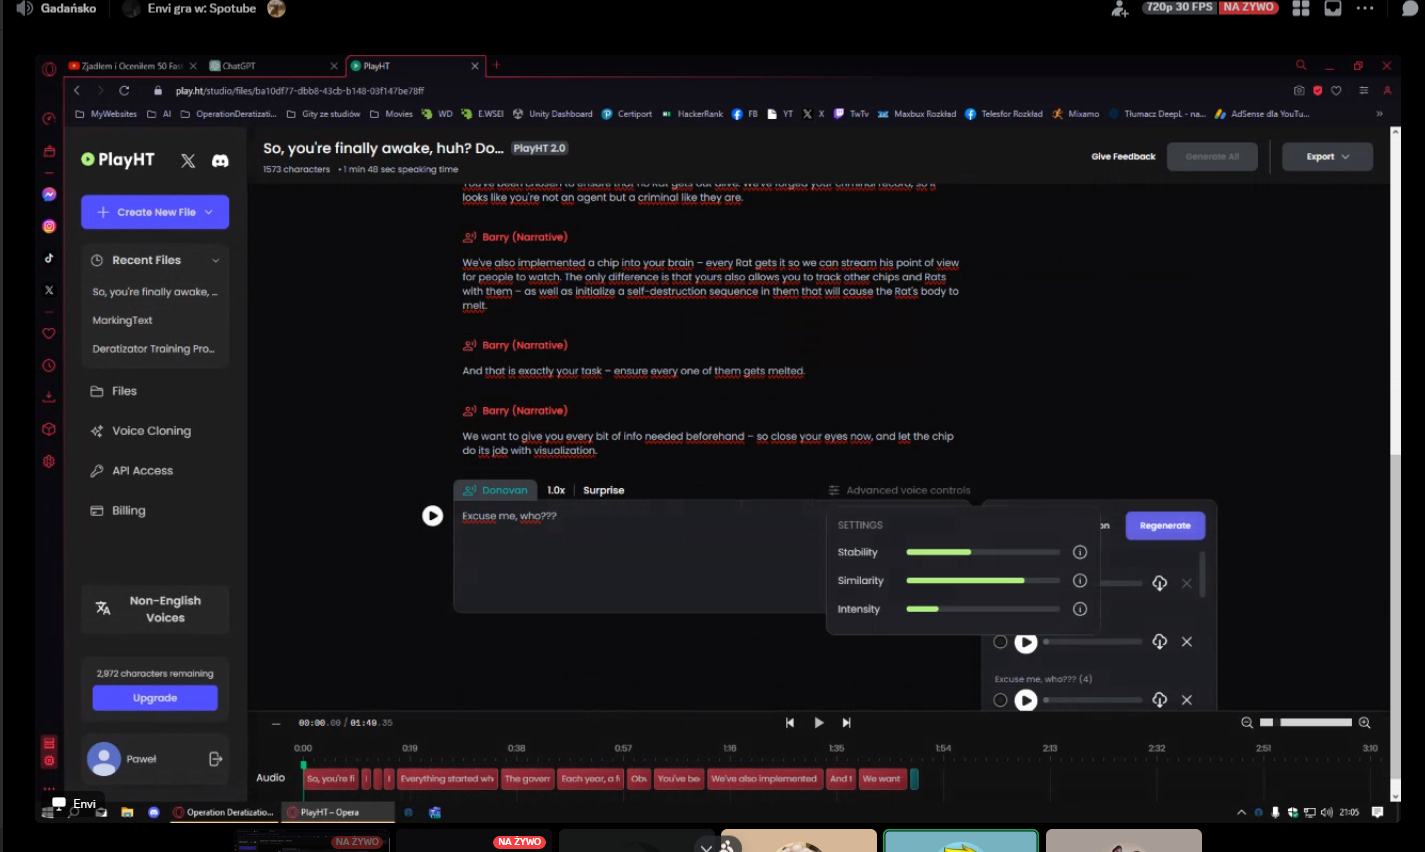
\includegraphics[width=0.5\linewidth]{Images/voice_hero.PNG}
    \caption{Konfiguracja głosu dla głównego bohatera}
    \label{fig:enter-label}
\end{figure}
\FloatBarrier
Dialogi zostały rozdzielone na oddzielne pliki - po jednym zdaniu per linijka.
Po umieszczeniu na timeline wszystkich dialogów, dostosowane zostało poruszanie się postaci.
\subsubsection{Cutscenka Intro - pozostałe w trakcie pracy}

Zamysł cutscenki stanowi rozwinięcie fabuły przedstawionej tutaj \nameref{game_description} \\
Cutscenka Intro ze względu na swoją strukture oraz historie przestawioną może zostać na dwie osobne sekcje - pierwszą, w domku, gdzie narratorem jest postać Maxa Blackthorna - którego osoba pozostaje dla gracza pewnego rodzaju zagadką, na podstawie dialogów można snuć domysł że jest to agent rządowy, który wdraża nas - graczy - w role którą pełnimy w rozgrywce.\\
Początek scenki informuje nas niebezpośrednio że wszystkie zdarzenia oglądane są z perspektywy postaci gracza - poprzez efekt zamykania i otwierania oka.\\
Efekt ten został osiągnięty poprzez 
Sugeruje nam to również że gracz mógł zostać porwany.
Następnie narrator odchodzi, a na ścianie za nim zostaje za pomocą animatora naniesiona grafika w Sprite2D - oraz aktywowane i dezaktywowane jest światło (Spot Light), co emituje efekt odtwarzania slajdów.
Pozostały fragment pierwszej części cutscenki sprowadza się do kolejnych linii dialogu oraz zmiany slajdów (wyłączanie i analogiczna animacja dla innych obiektów Sprite2D)\\
Końcowy dialog jest punktem przełomowy - gracz jest informowany o posiadaniu przez postac "chipa" w głowie - co stanowi uzasadnienie mechanik takich jak oznaczenie ciał przeciwników czy nawet użyty interface - dodatkowo wprowadzenie owego "chipu" jako postaci pozwala zmienić narratora i w naturalny sposób zaprezentować graczowi poziom - co odbywa sie w drugiej części intro\\
Druga część intro to pokazanie wszystkich lokacji oraz punktów zainteresowania - wraz z narracją wprowadzającą historie owych miejsc.\\
Głównym elementem zastosowanym w tej części cutscene jest użycie wielu wirtualnych kamer oraz przełączanie się między nimi - oraz zmiana ich rotacji wraz z czasem z poziomu Animatora.\\
W celu poprawy wrażeń wizualnych niektóre z kamer posiadają zablokowany punkt na który patrzą (Look At) - dzięki czemu rozwiązanie polegające na pokazanie całego poziomu stało się znacznie łatwiejsze - kamera porusza się dookoła mapy, patrząc na pusty obiekt znajdujący się idealnie w centrum.\\
Na potrzeby tej części sceny zmodyfikowany również został skrypt odpowiedzialny za kontrolę drzwi:
\begin{codebox}
\begin{lstlisting}[language={[Sharp]C}, label={listing:DoorMotionSensor.cs}]
public class DoorMotionSensor : MonoBehaviour
{
    // ... (Remaining part of the script)
    
    if (isUsingCameraCheck)
    {
        float distanceToCamera = Vector3.Distance(transform.position, vCamera.transform.position);
        distance.Add(distanceToCamera);
        CinemachineTrackedDolly dollyCart = vCamera.GetCinemachineComponent<CinemachineTrackedDolly>();
        
        if (dollyCart != null)
        {
            float pathPosition = dollyCart.m_PathPosition;
            
            if (pathPosition >= 3f && pathPosition <= 4f || pathPosition >= 4.1f && pathPosition <= 5f)
                count++;
        }
    }
            
    // ... (Remaining part of the script)
}
\end{lstlisting}
\end{codebox}
\captionof{lstlisting}{Zmiany sposobu kontrolowania drzwi w skrypcie DoorMotionSensor.cs}
dzięki czemu obiekt DollyCart był w stanie aktywować animację otwierania drzwi podczas "wjazdu" kamery do restauracji, gdzie takowe drzwi zostały użyte.
Następnie zakończenie scenki prowadzi do przekierowania i wczytania sceny \textbf{Tutorial} - na której gracz może zapoznać się z mechanikami już z poziomu rozgrywki.
\newpage

\section{Audio}\label{sec:audio}
Rozdział poświęcony dźwiękowi i audio w grach komputerowych zajmuje się kluczowymi aspektami związanymi z projektowaniem, implementacją i optymalizacją dźwięku w grach.
\subsection{Kontrola ścieżek dźwiękowych}
W tej sekcji znajdziesz informacje na temat zarządzania różnymi ścieżkami dźwiękowymi w grze. Możesz kontrolować poziom głośności bezpośrednio z gry lub menu głównego, przechodząc do ustawień i przesuwając suwak od kontroli głośności muzyki lub osobnego suwaka dla reszty dźwięków. Ustawienia te są zapisywane w \texttt{PlayerPrefs}, co umożliwia utrzymanie preferencji gracza nawet po wyłączeniu gry. \\

\textbf{Kontrola głośności} jest również dostępna za pośrednictwem \textit{Audio Mixerów}. Modyfikacja zmiennych dostępnych w \texttt{PlayerPrefs} umożliwia kontrolę głośności z poziomu gry. Warto zauważyć, że te zmienne są udostępniane (zielone zaznaczenie po prawej na rysunku poniżej) do kontrolowania z \textit{Audio Mixerów} poszczególnych elementów dźwiękowych z poziomu skryptu, który obsługuje slidery głośności dostępne dla użytkownika w ustawieniach. \\

Oprócz tego, masz możliwość dostosowania głośności i efektów dźwiękowych z poziomu sceny. Modyfikowanie suwaków \textit{Audio Mixerów} od głośności (czerwone zaznaczenie na obrazku poniżej) lub suwaków komponentów \textit{Audio Source} na poszczególnych obiektach pozwala na precyzyjną kontrolę dźwięków w trakcie rozgrywki.

\begin{figure}[h]
    \centering
    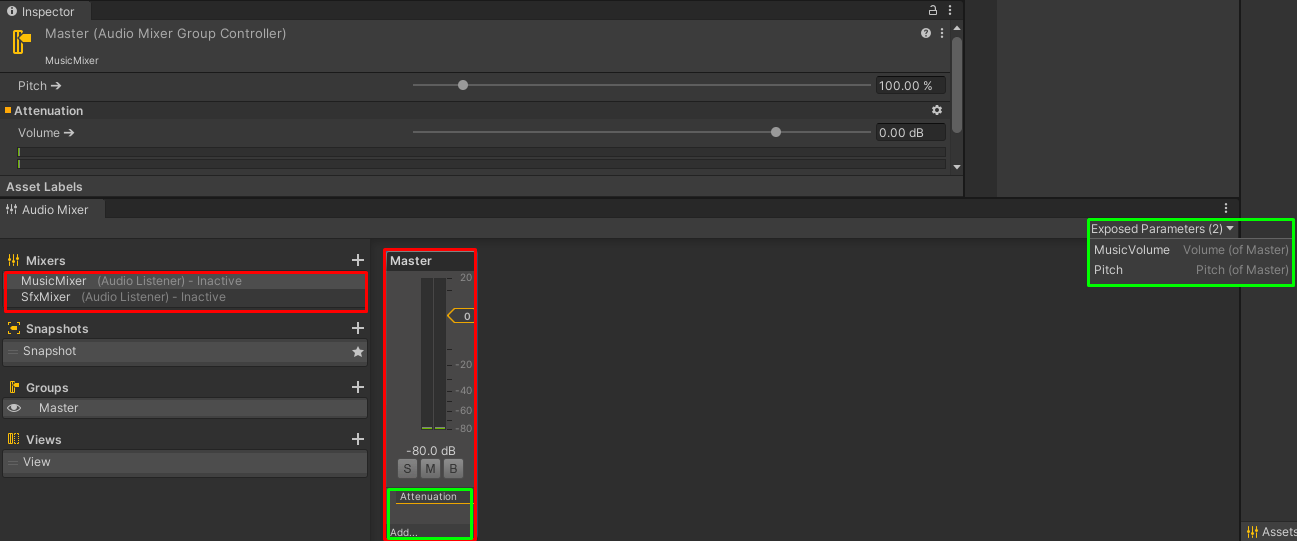
\includegraphics[width=1\linewidth]{Images/audioMixersSet.png}
    \caption{Ustawienia Audio Mixerów}
\end{figure}
\subsection{Ustawienia 3D dźwięków}
W sekcji dotyczącej ustawień 3D dźwięków, skupiamy się na implementacji efektów przestrzennych, które pomagają uzyskać bardziej realistyczne doznania dźwiękowe w grze. W przypadku naszej gry, kontrola nad efektami przestrzennymi staje się istotna dla zwiększenia immersji gracza.

Przykłady sytuacji, w których kontrola 3D dźwięków może być kluczowa:

\begin{enumerate}
    \item \textbf{Dźwięk broni:} Podczas strzelania z broni, efekty przestrzenne pozwalają na dokładne odwzorowanie źródła dźwięku w zależności od kierunku, w którym strzelasz. To może poprawić orientację gracza w otoczeniu oraz dostarczyć dodatkowych wrażeń związanych z użytkowaniem broni.
    \item \textbf{Dźwięk granatów:} Efekty przestrzenne umożliwiają precyzyjne określenie pozycji, w której eksplodował granat oraz odległości od naszego miejsca. Gracz będzie w stanie lepiej zrozumieć, czy zagrożenie pochodzi z przodu, tyłu czy z boku, co może wpłynąć na jego taktykę.
    \begin{figure}[h]
            \centering
            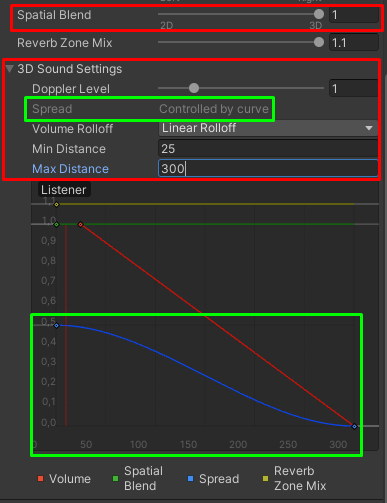
\includegraphics[scale=0.5]{Images/grenade3DSet.png}
            \caption{Przykładowe ustawienie 3D dźwięku dla obiektu granatu}
        \end{figure}
    \FloatBarrier
    W ustawieniach dźwięku 3D dla granatu, warto zwrócić uwagę na kilka kluczowych parametrów:
        \begin{itemize}
        \item \textbf{Spatial Blend:} Określa, jak bardzo dźwięk jest przestrzenny w stosunku do źródła. Wartość 1 oznacza, że dźwięk jest w pełni przestrzenny, natomiast wartość 0 oznacza, że dźwięk jest zupełnie dwuwymiarowy.
        \item \textbf{3D Sounds Settings:} Pozwala na dostosowanie wielu parametrów dźwięku przestrzennego, takich jak odległość, w jakiej dźwięk słychać, szybkość spadku głośności w zależności od odległości czy także szybkość przemieszczania się dźwięku.
        \item \textbf{Spread:} Określa rozproszenie dźwięku, czyli jak szeroko dźwięk jest rozprzestrzeniony w przestrzeni. Wartość 0 oznacza brak rozproszenia, a wartość 360 oznacza pełne rozproszenie wokół źródła dźwięku.
        \end{itemize}
    \item \textbf{Dźwięk otwieranych skrzynek:} Kontrola 3D dźwięków może pomóc w tworzeniu bardziej realistycznego doświadczenia podczas otwierania skrzynek czy innych kontenerów. Dźwięk tych elementów będzie można precyzyjnie zlokalizować w przestrzeni, co dodatkowo podniesie realizm gry.
    \item \textbf{Dźwięk drzwi:} Efekty przestrzenne pozwalają na dokładne odwzorowanie dźwięku otwieranych drzwi. Gracz będzie w stanie odróżnić, czy drzwi otwierają się po lewej czy prawej stronie, co może mieć znaczenie taktyczne w przypadku szybkiego przemieszczania się po lokacji.
\end{enumerate}

\newpage

\section{Testowanie i debugowanie}\label{sec:test}
Rozdział o testowaniu stanowi kluczową część procesu tworzenia oprogramowania, obejmującą różnorodne strategie, metody i narzędzia służące zapewnieniu jakości produktu. Testowanie jest nieodłącznym elementem każdego projektu, bez względu na jego skalę czy rodzaj. Ten rozdział skupia się na zasadach i praktykach związanych z testowaniem w kontekście tworzenia gier komputerowych. Omówimy różne strategie testowania, które pomogą zapewnić wysoką jakość gry oraz zidentyfikować potencjalne problemy jeszcze przed wykonaniem ostatecznego buildu. \\ \\
W rozdziale omówione zostaną różne aspekty testowania, począwszy od planowania strategii testowej, przez wykorzystane narzędzia testerskie, aż po analizę wyników i raportowanie błędów. Podkreślona zostanie rola testowania w zapewnianiu jakości oprogramowania, identyfikowaniu i usuwaniu błędów oraz poprawianiu doświadczenia użytkownika.
\subsection{Strategie testowania}
Testowanie gry pierwszoosobowej jest kluczowym etapem rozwoju, mającym na celu zapewnienie płynności rozgrywki, stabilności oraz satysfakcji graczy. W tym rozdziale omówimy różne strategie testowania, które pomogą zapewnić wysoką jakość gry oraz zidentyfikować potencjalne problemy jeszcze przed wykonaniem ostatecznego buildu.
\subsection{Narzędzia debugujące}
W procesie tworzenia gry FPS na silniku Unity kluczowym elementem jest skuteczne debugowanie, czyli identyfikowanie, analizowanie i rozwiązywanie błędów w kodzie i mechanice gry. Poniżej przedstawione zostaną niektóre z najważniejszych narzędzi debugujących, które mogą być wykorzystane w tym kontekście.

\paragraph{Unity Profiler}\hspace{-1em} -- to narzędzie, które pozwala na analizę wydajności gry. Pomaga identyfikować miejsca, gdzie gra zużywa najwięcej zasobów komputera (GPU, CPU i pamięć RAM). Dla naszej gry Profiler jest niezastąpiony przy optymalizacji wydajności renderowania i skryptów odpowiedzialnych za obsługę mechanik.

\begin{figure}[h]
        \centering
        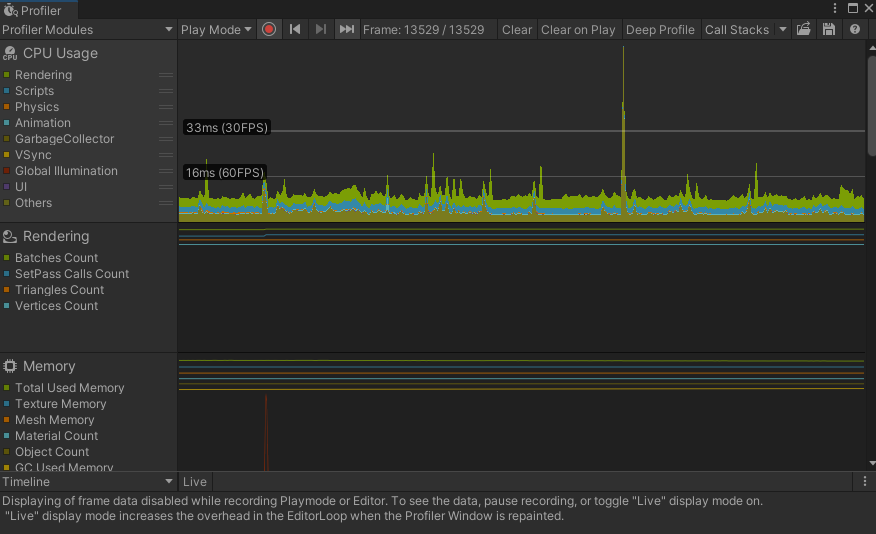
\includegraphics[width=0.9\linewidth]{Images/profiler}
        \caption{Okno Profilera dostępnego w edytorze Unity}
\end{figure}
\FloatBarrier
\paragraph{Unity Frame Debugger}\hspace{-1em} -- to narzędzie dostępne w środowisku Unity, które umożliwia programistom analizę renderowania klatki gry. Jest to szczególnie ważne w grach FPS, gdzie płynność i wydajność renderowania mają kluczowe znaczenie dla doświadczenia gracza.

\begin{figure}[h]
        \centering
        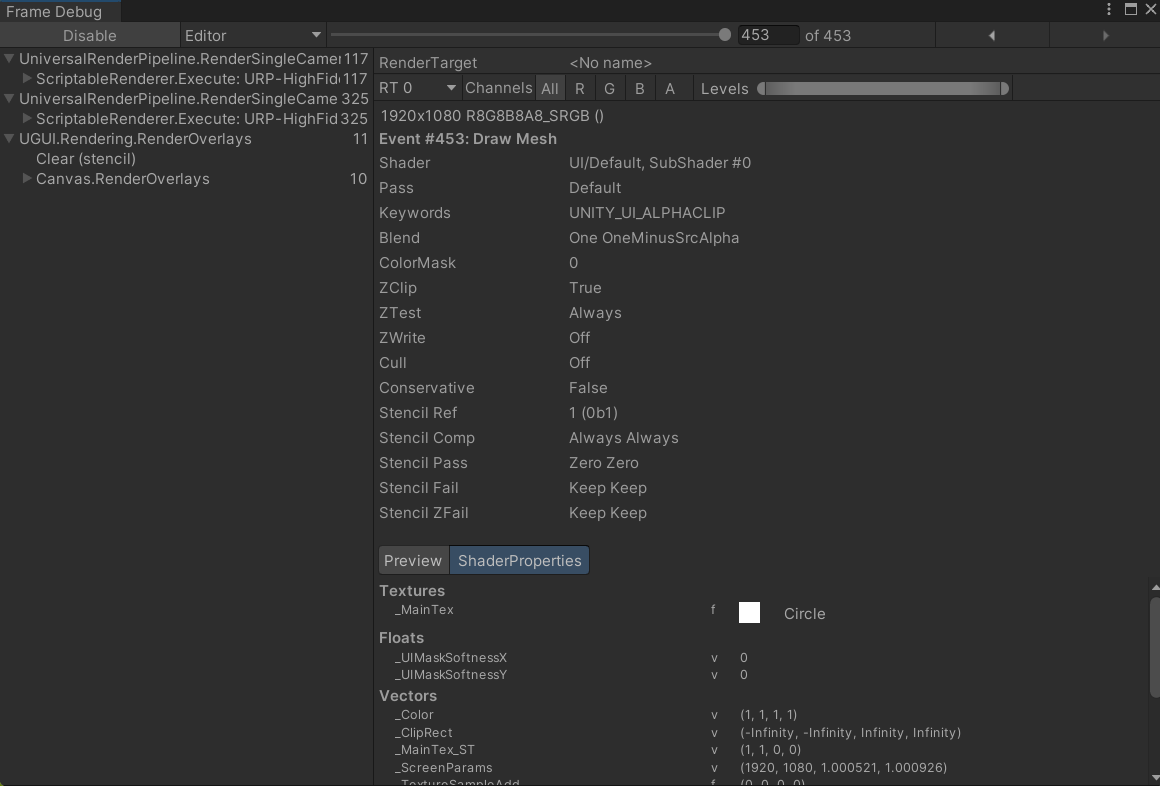
\includegraphics[width=0.9\linewidth]{Images/frameDebug.png}
        \caption{Okno Frame Debuggera w edytorze Unity}
\end{figure}
\FloatBarrier
\paragraph{Unity Console}\hspace{-1em} -- Bardzo prosta ale przydatna konsola dostępna bezpośrednio w edytorze Unity. Wyświetla komunikaty, ostrzeżenia oraz błędy co ułatwia śledzenie zmian i problemów w grze. Konsola bardzo pomaga w identyfikacji problemów związanych z interakcjami z otoczeniem czy działaniem broni.

\begin{figure}[h]
        \centering
        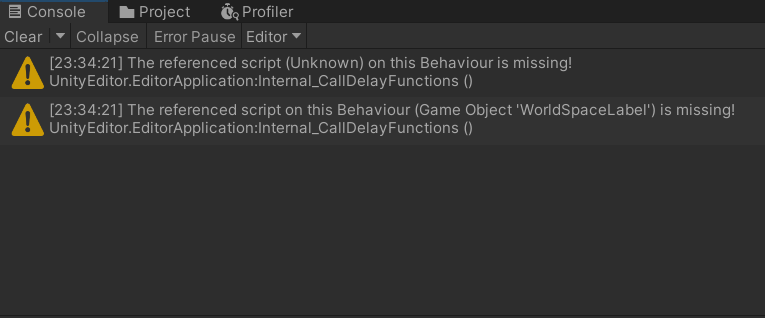
\includegraphics[width=0.9\linewidth]{Images/console.png}
        \caption{Okno Console w edytorze Unity}
\end{figure}
\FloatBarrier
\subsection{Raportowanie błędów}
Rozwój gier wideo to złożony proces, który wymaga nieustannej uwagi i zaangażowania zespołu programistycznego. Jednym z kluczowych elementów tego procesu jest skuteczne zarządzanie i monitorowanie błędów, które mogą pojawić się podczas różnych faz produkcji. Trello, jako narzędzie do zarządzania projektami, może stanowić doskonałe wsparcie w raportowaniu i śledzeniu błędów w grze. Poniżej omówiony zostanie sposób zastosowania Trello w naszym projekcie.

\paragraph{Dev Bug List}\hspace{-1em} -- Na tej liście dodajemy karty ze zgłoszeniami błędów deweloperskich, które zostały odkryte i należy je naprawić. W karcie wybieramy etykietę \textit{Bug} oraz ewentualnie \textit{Important} jeżeli zgłoszenie ma wysoki priorytet i wybieramy kategorię, której dotyczy błąd (np.  \textit{Mechaniki} lub  \textit{Audio}). Następnie dodajemy opis, z którym musi zapoznać się deweloper jeżeli błąd jest złożony. Podpinamy się do zadania jako osoba zgłaszająca, a programista podpina się do taska samodzielnie. Wewnątrz karty z zadaniem możemy śledzić co w tym momencie dzieje się z tematem, który zgłosiliśmy poprzez zapoznanie się z komentarzami dewelopera.
\begin{figure}[h]
    \centering
    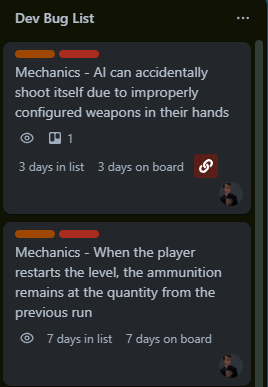
\includegraphics[scale=0.7]{Images/devBuglist.png}
    \caption{Lista rozpoznanych błędów deweloperskich występujących w grze}
    \label{fig:devBuglist}
\end{figure}
\paragraph{Visual Bug List}\hspace{-1em} -- Na tą listę trafiają zgłoszenia rozpoznanych błędów wizualnych, które należy naprawić. Podobnie jak w przypadku karty z błędami deweloperskimi w karcie wybieramy odpowiednie etykiety, dodajemy opis dla osoby, która będzie odpowiedzialna za naprawę błędu. Następnie podpinamy się do karty jako zgłaszający i czekamy aż osoba odpowiedzialna za naprawienia buga się do niej przypnie sama. Wewnątrz karty sprawdzimy postęp naprawy.
\begin{figure}[h]
    \centering
    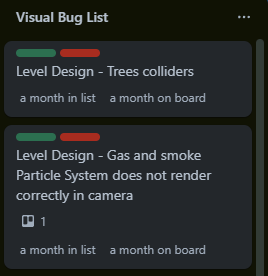
\includegraphics[scale=0.7]{Images/visBuglist.png}
    \caption{Lista rozpoznanych błędów wizualnych występujących w grze}
    \label{fig:visBuglist}
\end{figure}
\FloatBarrier
Osoba odpowiedzialna za naprawę błędu po zaznajomieniu się z zadaniem przenosi kartę do listy \textbf{Work In Progress}. \\
Po naprawie błędu osoba odpowiedzialna za niego przerzuca go do listy \textbf{Internal Test}, gdzie tester lub osoba zgłaszająca problem sprawdza czy błąd rzeczywiście udało się wyeliminować i czy przy okazji nie powstał z tego powodu inny bug:
\begin{itemize}
    \item W przypadku, gdzie problem został naprawiony i pomyślnie przeszedł testy karta z zadaniem zostaje przeniesiona do \textbf{Done} i cykl życia taska się zamyka.
    \item W przypadku, gdzie problem nie został naprawiony/powoduje innego rodzaju problemy karta z zadaniem zostaje przeniesiona do listy \textbf{Work In Progress} ze stosownym komentarzem dla osoby odpowiedzialnej za ten task (co nie zadziałało/jak odtworzyć błąd/jaka inna mechanika przestała działać po zmianach).
\end{itemize}

\newpage

\section{Optymalizacja i wydajność}\label{sec:opt}
Optymalizacja stanowi kluczowy element procesu tworzenia gry w środowisku Unity, skupiając się na poprawie efektywności działania i zapewnieniu płynności doświadczenia gracza. W obrębie tego rozdziału, eksplorujemy różnorodne aspekty optymalizacji, koncentrując się na trzech głównych sekcjach, które znajdziesz poniżej.
\subsection{Profilowanie kodu}
Profilowanie kodu jest kluczowym etapem w procesie optymalizacji. W tej sekcji przedstawimy i omówimy narzędzia dostępne w środowisku Unity do analizy wydajności kodu, a także skonfigurujemy profiler w celu efektywnego monitorowania wydajności. \\ \\
Unity udostępnia zaawansowane narzędzia do profilowania kodu, pozwalające na analizę wydajności w różnych aspektach. Poniżej przedstawiamy kluczowe narzędzia wbudowane w Unity:

\begin{itemize}
    \item \textbf{Profiler Unity} - Profiler to narzędzie, umożliwiające śledzenie i analizę wydajności podczas działania gry lub z okna edytora po przełączeniu trybu na \textit{Edit Mode}. Pozwala ono na monitorowanie zużycia zasobów, czasu renderowania, czasu CPU, alokacji pamięci i innych parametrów, których widoczność możemy przełączać klikając w \textit{Profiler Modules} w oknie Profilera.
    \begin{figure}[h]
        \centering
        \includegraphics[width=1\linewidth]{Images/unityProfiler.png}
        \caption{Okno Profilera dostępne w menu kontekstowym Window/Analysis/Profiler}
    \end{figure}
    \item \textbf{Unity Frame Debugger} - Frame Debugger pozwala na dokładną analizę, jak Unity renderuje każdą klatkę. Wystarczy kliknąć przycisk \textit{Enable} w oknie Frame Debug i wybrać interesującą nas klatkę. To narzędzie jest szczególnie przydatne do identyfikacji problemów związanych z grafiką i renderowaniem.
    \begin{figure}[h]
        \centering
        \includegraphics[width=1\linewidth]{Images/frameDebugger.png}
        \caption{Okno Frame Debug, które znajdziemy w menu kontekstowym Window/Analysis/Frame Debugger}
    \end{figure}
    \FloatBarrier
\end{itemize}
\subsection{Zarządzanie zasobami}
Wydajne zarządzanie zasobami jest kluczowym aspektem zapewnienia płynności działania gry. W tym podrozdziale omówimy strategie ładowania i zwalniania zasobów w zależności od potrzeb sceny. Przyjrzymy się tematom takim asynchroniczne ładowanie czy korzyści płynące z użycia wzorca \textit{puli obiektów}.

\subsubsection{Asynchroniczne Ładowanie}
Asynchroniczne ładowanie sceny jest kluczowym elementem optymalizacji gier, umożliwiając płynne przejścia między różnymi fragmentami rozgrywki. W tym kontekście przedstawiamy skrypt \texttt{SceneLoader.cs}, który implementuje asynchroniczne ładowanie sceny w grze.
\begin{codebox}
\begin{lstlisting}[language={[Sharp]C}, label={listing:SceneLoader.cs}]
public class SceneLoader : MonoBehaviour
{
    // ... (Remaining part of the script)

    public IEnumerator LoadScene_Coroutine(int index)
    {
        AsyncOperation asyncOperation = SceneManager.LoadSceneAsync(index);
        asyncOperation.allowSceneActivation = false;
        float progress = 0;
        
        while (!asyncOperation.isDone)
        {
            progress = Mathf.MoveTowards(progress, asyncOperation.progress, Time.deltaTime);
            progressSlider.value = progress;
            
            if (progress >= 0.9f)
            {
                progressSlider.value = 1;
                asyncOperation.allowSceneActivation = true;
            }
            
            yield return null;
        }
    }
}
\end{lstlisting}
\end{codebox}
\captionof{lstlisting}{Klasa SceneLoader obsługująca asynchroniczne przechodzenie między scenami}
Skrypt ten umożliwia dynamiczne ładowanie sceny, co jest szczególnie użyteczne przy dużych i rozbudowanych projektach. Kluczowym elementem jest użycie klasy \texttt{AsyncOperation}, która pozwala na asynchroniczne ładowanie sceny w tle, bez blokowania głównego wątku gry.
\textbf{Elementy kluczowe skryptu:}
\begin{itemize}
\item \textbf{LoaderUI:} Obiekt reprezentujący interfejs użytkownika (UI) wykorzystywany podczas ładowania sceny.
\item \textbf{progressSlider:} Pasek postępu ładowania sceny, umożliwiający informowanie gracza o aktualnym stanie procesu.
\item \textbf{gOToDeactivate:} Obiekt do dezaktywacji podczas ładowania sceny, co może być przydatne, aby ukryć niepotrzebne elementy w trakcie przejścia między scenami.
\item \textbf{LoadScene:} Metoda rozpoczynająca proces ładowania sceny. Wywołuje \texttt{LoadScene\_Coroutine} w ramach coroutine.
\item \textbf{LoadScene\_Coroutine:} Coroutine odpowiedzialna za asynchroniczne ładowanie sceny. W trakcie procesu aktualizuje pasek postępu, a po osiągnięciu 90\% pozwala na aktywację sceny.
\end{itemize}
Użycie asynchronicznego ładowania sceny poprzez ten skrypt pozwala na zachowanie płynności rozgrywki nawet w przypadku dużych i złożonych scen, jednocześnie umożliwiając informowanie gracza o postępie za pomocą paska ładowania. Skrypt osiąga stan 90\% ładowania, a następnie pozwala na aktywację sceny. Ograniczenie ładowania do 90\% zanim scena zostanie aktywowana ma na celu zminimalizowanie zakłóceń związanych z ostatecznym przejściem do nowej sceny, umożliwiając jednocześnie aktualizację interfejsu użytkownika i przygotowanie do gry. Jest to istotny element optymalizacji, który przyczynia się do lepszych doświadczeń graczy.

\subsubsection{Object Pooling}
\textit{Object Pooling} umożliwia efektywne ponowne wykorzystanie obiektów w grze, zamiast dynamicznego tworzenia i niszczenia ich. Podejście to pomaga zminimalizować obciążenie systemu, zwłaszcza w przypadku obiektów, które są często tworzone i usuwane, takich jak efekty cząsteczkowe, wskaźniki obrażeń, popupy z obrażeniami czy rany po pociskach. \\ \\
Skrypt \texttt{ObjectPoolManager.cs} jest centralnym elementem zarządzającym pulą obiektów. Jeżeli interesuje Cię sama implementacja funkcji do tworzenia puli obiektów oraz tej odpowiedzialnej za ich powrót do puli to sugerujemy powrót do podsekcji \nameref{subsubsec:objPoolPattern} gdzie możesz znaleźć code snippet, którego szukasz! Poniżej przedstawiono główne funkcje skryptu:
\begin{itemize}
    \item \textbf{SpawnObject:} Funkcja ta służy do tworzenia obiektów z puli. Sprawdza, czy dany obiekt już istnieje w puli. Jeśli nie, tworzy nowy obiekt; jeśli tak, ponownie go aktywuje i umieszcza na odpowiedniej pozycji.
    \item \textbf{ReturnObjectToPool:} Funkcja odpowiada za zwrot obiektu do puli po zakończeniu jego używania. Obiekt jest dezaktywowany i dodawany z powrotem do puli.
    \item \textbf{SetParentObject:} Funkcja ta ustawia rodzica dla danego obiektu w zależności od jego typu. Pomaga to w utrzymaniu porządku w hierarchii obiektów w scenie.
\end{itemize}
Dodatkowo, skrypty które znajdziesz poniżej prezentują konkretne przypadki użycia \textit{puli obiektów} w akcji: \label{subsubsec:objPoolExamples}
\begin{itemize}
    \item Skrypt \textbf{ReturnParticlesToPool.cs:} Skrypt ten reprezentuje konkretny przypadek użycia \textit{puli obiektów} w kontekście efektów cząsteczkowych. Po zakończeniu emisji cząsteczek wywołuje funkcję zwracającą obiekt do puli.
    \begin{codebox}
    \begin{lstlisting}[language={[Sharp]C}, label={listing:ReturnParticlesToPool.cs}]
    public class ReturnParticlesToPool : MonoBehaviour
    {
        private void OnParticleSystemStopped()
        {
            ObjectPoolManager.ReturnObjectToPool(gameObject);
        }
    }
    \end{lstlisting}
    \end{codebox}
    \captionof{lstlisting}{Zwrócenie obiektu do puli po zakończeniu trwania efektu systemu cząsteczkowego}
\end{itemize}
\begin{itemize}
    \item Skrypt \textbf{ReturnToPoolAfterTimer.cs} Ten skrypt ilustruje użycie \textit{puli obiektów} w kontekście czasowego zwalniania zasobów. Po aktywowaniu obiektu, rozpoczyna odliczanie czasu i po upływie określonego czasu, zwraca obiekt do puli.
    \begin{codebox}
    \begin{lstlisting}[language={[Sharp]C}, label={listing:ReturnToPoolAfterTimer.cs}]
    public class ReturnToPoolAfterTimer : MonoBehaviour
    {
        public float timeToDespawn = 1f;
        private Coroutine _timerCoroutine;

        private void OnEnable()
        {
            _timerCoroutine = StartCoroutine(ReturnToPoolAfterTime());
        }
        private IEnumerator ReturnToPoolAfterTime()
        {
            float elapsedTime = 0f;

            while(elapsedTime < timeToDespawn)
            {
                elapsedTime += Time.deltaTime;
                yield return null;
            }

            ObjectPoolManager.ReturnObjectToPool(gameObject);
        }
    }
    \end{lstlisting}
    \end{codebox}
    \captionof{lstlisting}{Zwrócenie obiektu do puli po upływie określonego czasu}
\end{itemize}
\begin{itemize}
    \item Skrypt \textbf{ReturnToPoolOnAnimationEnd.cs:} Skrypt ten prezentuje wykorzystanie \textit{puli obiektów} w kontekście zwalniania zasobów po zakończeniu animacji. Po zakończeniu animacji obiektu, rodzic tego obiektu zostaje zwrócony do puli.
    \begin{codebox}
    \begin{lstlisting}[language={[Sharp]C}, label={listing:ReturnToPoolOnAnimationEnd.cs}]
    public class ReturnToPoolOnAnimationEnd : MonoBehaviour
    {
        public void DestroyParent()
        {
            GameObject parentObject = gameObject.transform.parent.gameObject;
            ObjectPoolManager.ReturnObjectToPool(parentObject);
        }
    }
    \end{lstlisting}
    \end{codebox}
    \captionof{lstlisting}{Klasa ReturnToPoolOnAnimationEnd wykorzystywana do zwrócenia obiektu do puli po zakończeniu trwania animacji przy użyciu zdarzeń animacji Unity}
\end{itemize}
Poniżej znajdziesz konfiguracje obiektów w zależności od sposobu w jaki możesz je dodać do systemu \textit{puli obiektów} oraz przykład podmiany wbudowanych i kosztownych funkcji silnika Unity, czyli \textit{Instantiate} oraz \textit{Destroy}.
\begin{figure}[h]
    \centering
    \includegraphics[scale=0.55]{Images/particlesObjPoolSetup.png}
    \caption{Konfiguracja obiektu Particle System, który powinien wrócić do puli obiektów po zakończeniu emisji cząsteczek}
\end{figure}
\FloatBarrier
\begin{figure}[h]
    \centering
    \includegraphics[width=0.5\linewidth]{Images/timerObjPoolSetup.png}
    \caption{Konfiguracja obiektu, który ma wrócić do puli obiektów po upływie czasu}
\end{figure}
\FloatBarrier
\begin{figure}[h]
    \centering
    \includegraphics[width=1\linewidth]{Images/animObjPoolSetup.png}
    \caption{Konfiguracja obiektu, który ma wrócić do puli obiektów po zakończeniu odtwarzania animacji}
\end{figure}
\FloatBarrier
\begin{figure}[h]
    \begin{codebox}
    \begin{lstlisting}[language={[Sharp]C}, label={listing:DISystem.cs}]
    public class DISystem : MonoBehaviour
    {
        [SerializeField] private GameObject indicatorPrefab;
        [SerializeField] private RectTransform holder;

        // ... (Remaining part of the script)
        
        private void Create(Transform target)
        {
            // ... (Remaining part of the function)

            GameObject indicator = ObjectPoolManager.SpawnObject(indicatorPrefab, Vector3.zero, Quaternion.identity, holder);
            
            // ... (Remaining part of the function)
        }
    }
    \end{lstlisting}
    \end{codebox}
    \captionof{lstlisting}{Przykład podmiany funkcji Instantiate w skrypcie DISystem.cs na nowo utworzoną i zoptymalizowaną SpawnObject z klasy ObjectPoolManager}
\end{figure}
\begin{figure}[h]
    \begin{codebox}
    \begin{lstlisting}[language={[Sharp]C}, label={listing:DamageIndicator.cs}]
    public class DamageIndicator : MonoBehaviour
    {
        // ... (Remaining part of the script)
        
        private IEnumerator Countdown()
        {
            // ... (Remaining part of the function)

            unRegister();
            ObjectPoolManager.ReturnObjectToPool(gameObject);
        }
    }
    \end{lstlisting}
    \end{codebox}
    \captionof{lstlisting}{Przykład podmiany funkcji Destroy w skrypcie DamageIndicator.cs na nowo utworzoną i zoptymalizowaną ReturnObjectToPool z klasy ObjectPoolManager}
\end{figure}
\subsection{Techniki optymalizacji wydajności}
\subsubsection{Wyszukiwanie Obiektów}
Podczas programowania w Unity, efektywne wyszukiwanie obiektów w scenie jest kluczowe dla wydajności gry. Unikamy zasobożernych funkcji, takich jak \textbf{FindObjectOfType}, szczególnie w każdej klatce, aby uniknąć zbędnego obciążenia. Ostatecznie wyeliminowaliśmy wszystkie użycia tej funkcji z kilku prostych powodów, ale m.in. dlatego, że funkcja ta przeszukuje całą scenę (mówimy tu o wszystkich obiektach gry i o wszystkich ich komponentach!) oraz nie jest ograniczona do konkretnego obszaru lub hierarchii.\\ \\
Zamiast tego, zalecamy korzystanie z bardziej efektywnych metod, takich jak:
\begin{itemize}
    \item \textbf{Bezpośrednie Referencje w Edytorze Unity:} Przypisywanie referencji bezpośrednio w inspektorze Unity może być bardzo efektywne. Jeśli dany obiekt jest dostępny bezpośrednio poprzez referencję, nie trzeba korzystać z funkcji wyszukujących.
    \item \textbf{GetChild:} Funkcja pozwalająca na odnalezienie konkretnego dziecka obiektu, co jest przydatne, gdy hierarchia obiektów jest złożona.
    \item \textbf{GetComponent:} Pozwala na bezpośrednie odnalezienie komponentu przypisanego do obiektu. Jest to efektywna metoda, zwłaszcza gdy wiemy, że dany obiekt posiada określony komponent.
    \item \textbf{GetComponentInParent:} Metoda umożliwiająca znalezienie komponentu w hierarchii rodzica obiektu.
    \item \textbf{GetComponentInChildren:} Funkcja wyszukująca komponenty wśród dzieci danego obiektu.
    \item \textbf{FindGameObjectWithTag:} Efektywne wyszukiwanie obiektów po tagu. Jest to skuteczna metoda, jeśli obiekty są odpowiednio oznaczone tagami.
    \item \textbf{Find:} Możemy używać ogólnego wyszukiwania obiektów, takiego jak Find, w celu znalezienia obiektu po jego nazwie. Należy jednak używać go z umiarem, aby uniknąć nadmiernego obciążenia.
\end{itemize}
Optymalnym rozwiązaniem jest również projektowanie systemu, w którym unikamy częstego wyszukiwania obiektów w czasie rzeczywistym. Zamiast tego, stosujmy strategie takie jak cachowanie referencji, używanie menedżerów lub struktur organizacyjnych w scenie, aby minimalizować liczbę operacji wyszukiwania. To podejście przyczyni się do płynności działania gry, zwłaszcza w przypadku dużych projektów.
\begin{figure}[h]
    \centering
    \includegraphics[width=1\linewidth]{Images/findObjectsOptimization.png}
    \caption{Optymalizacja pozyskiwania obiektów - porzucenie wywołań FindObjectOfType}
\end{figure}
\FloatBarrier

\subsubsection{Konstruktor Łańcucha Znaków}
\textbf{String Builder} to klasa w języku C\#, która umożliwia dynamiczne tworzenie, manipulowanie i modyfikowanie łańcuchów znaków. Główną różnicą między String Builder a standardowymi łańcuchami znaków (typ string) jest to, że String Builder jest mutowalny, co oznacza, że można go modyfikować bez tworzenia nowych instancji obiektów za każdym razem, gdy dokonywane są zmiany. \\ \\
\begin{enumerate}
    \item \textbf{Zalety String Buildera}
        \begin{itemize}
        \item \textbf{Efektywność pamięciowa:} W przypadku operacji na łańcuchach znaków, szczególnie gdy wymagane są powtarzane modyfikacje, String Builder oferuje znaczną efektywność pamięciową. Ponieważ obiekty typu string są niemodyfikowalne, każda operacja modyfikacji tworzy nowy obiekt. String Builder minimalizuje ten problem, pozwalając na modyfikację istniejącego obiektu bez konieczności tworzenia nowego za każdym razem.
        \item \textbf{Szybkość operacji modyfikacji:} Operacje modyfikacji, takie jak dodawanie, usuwanie lub zamiana znaków, są szybsze w przypadku String Builder niż dla typu string. W przypadku typu string, każda operacja modyfikacji tworzy nowy obiekt, co wpływa na wydajność, szczególnie w przypadku dużej liczby operacji.
        \item \textbf{Efektywność czasowa:} Dla operacji, które wymagają wielokrotnych modyfikacji, String Builder jest bardziej efektywny czasowo niż konkatenacja łańcuchów znaków (string + string). Konkatenacja za każdym razem tworzy nowy obiekt, co może prowadzić do kosztownych operacji kopiowania danych.
        \end{itemize}
    \item \textbf{Zastosowanie String Buildera}
        \begin{itemize}
        \item \textbf{Budowanie długich łańcuchów znaków:} Jeśli musisz dynamicznie budować długi łańcuch znaków, String Builder jest bardziej efektywny niż konkatenacja standardowych łańcuchów.
        \item \textbf{Częste modyfikacje tekstu:} W przypadku, gdy tekst podlega częstym zmianom, a konieczność tworzenia nowych obiektów jest nieefektywna, String Builder pozwala na płynne modyfikacje bez nadmiernego obciążenia pamięciowego.
        \item \textbf{Wydajne składanie wiadomości lub komunikatów:} W przypadku tworzenia komunikatów, logów lub innych dynamicznych komunikatów tekstowych, String Builder umożliwia efektywne tworzenie i modyfikowanie treści.
        \end{itemize}
    \item \textbf{Tworzenie Obiektu String Buildera}
        String Builder może być inicjowany różnymi sposobami. Poniżej przedstawiono jedną z metod tworzenia obiektu String Builder:
        \begin{verbatim}
            StringBuilder stringBuilder = new StringBuilder();
        \end{verbatim}
        Ten konstruktor tworzy pusty obiekt String Builder, który może być następnie modyfikowany przez różne operacje, takie jak dodawanie, usuwanie czy zamiana znaków.
        \begin{figure}[h]
            \centering
            \includegraphics[width=1\linewidth]{Images/stringBuilder.png}
            \caption{Optymalizacja modyfikowania ciągów znaków - zastosowanie String Buildera}
        \end{figure}
\end{enumerate}
\FloatBarrier

\subsubsection{Pola Statyczne Obiektów}
Pola statyczne mogą być używane w celu przechowywania danych, które są wspólne dla wszystkich instancji danej klasy. Omówimy, kiedy i jak używać pól statycznych w celu zoptymalizowania zarządzania danymi w grze.
\begin{figure}[h]
    \centering
    \includegraphics{Images/staticField.png}
    \caption{Odpowiednie wykorzystanie pola Static na obiekcie}
\end{figure}
\paragraph{Opcje Statycznych Pól Obiektów w Unity}\hspace{-1em} -- Statyczne pola obiektów w Unity oferują kilka opcji do kontrolowania zachowania obiektu w scenie. Oto opcje i ich znaczenia:
\begin{itemize}
    \item \textbf{Nothing:} Obiekt nie przyczynia się do statycznego zbiorczego renderowania (batching), eliminowania elementów niewidocznych (occlusion culling) ani globalnego oświetlenia (GI).
    \item \textbf{Everything:} Obiekt uczestniczy w batchingu, occlusion cullingu oraz GI.
    \item \textbf{Contribute GI:} Obiekt przyczynia się do obliczeń GI, ale nie uczestniczy w batchingu ani occlusion cullingu.
    \item \textbf{Occluder Static:} Obiekt działa jako zakrywacz dla statycznych obliczeń occlusion culling.
    \item \textbf{Batching Static:} Obiekt uczestniczy w batchingu, ale nie w GI ani occlusion cullingu.
    \item \textbf{Navigation Static:} Obiekt jest uwzględniany w generowaniu statycznej siatki nawigacyjnej.
    \item \textbf{Occludee Static:} Obiekt jest brany pod uwagę w occlusion cullingu, ale nie działa jako zakrywacz.
    \item \textbf{Off Mesh Link Generation:} Obiekt jest uwzględniany w generowaniu połączeń międzymeshowych dla nawigacji.
    \item \textbf{Reflection Probe Static:} Obiekt przyczynia się do statycznych obliczeń sond odbicia.
\end{itemize}

\subsubsection{Pola GPU Instancing}
Aktywowanie opcji GPU Instancing dla powtarzających się obiektów umożliwia renderowanie ich jednym wywołaniem, co przyśpiesza proces renderowania. Poniżej przedstawiamy konfigurację materiału w celu zastosowania tej techniki.
\begin{figure}[h]
    \centering
    \includegraphics[width=0.85\linewidth]{Images/gpuInstanceOptimization.png}
    \caption{Renderowanie obiektów z użyciem GPU Instancing}
\end{figure}

\subsubsection{Wypiekanie Świateł} \label{subsubsec:bakingLights}
Wypiekanie świateł to proces wstępnych obliczeń oświetlenia, co może znacznie poprawić wydajność renderowania w czasie rzeczywistym. Przedstawimy korzyści i kroki do przeprowadzenia wypiekania świateł w projekcie.
\begin{itemize}
    \item \textbf{Poprawiona Wydajność Renderowania w Czasie Rzeczywistym:} Poprzez wstępne obliczenia informacji oświetleniowej, zmniejsza się konieczność obliczeń w czasie rzeczywistym podczas rozgrywki, co przekłada się na płynniejszą wydajność renderowania.
    \item \textbf{Spójność Oświetlenia:} Wypiekanie świateł zapewnia spójność oświetlenia pomiędzy scenami, poprawiając jednolity wygląd i utrzymując bardziej wyszukany charakter wizualny.
    \item \textbf{Zwiększone Detale i Cienie: } Wypiekanie oświetlenia pozwala uzyskać skomplikowane detale i realistyczne cienie, przyczyniając się do bardziej immersyjnego i atrakcyjnego otoczenia.
    \item \textbf{Optymalizacja dla Urządzeń Nisko-Wydajnych:} Wypiekanie świateł może być szczególnie korzystne dla optymalizacji projektów skierowanych na urządzenia nisko-wydajne, zapewniając lepsze doświadczenie użytkownika na różnych rodzajach sprzętu.
    \item \textbf{Przewidywalne Wyniki Oświetleniowe:} Ponieważ oświetlenie jest wstępnie obliczane, można osiągnąć przewidywalne i możliwe do odtworzenia wyniki oświetleniowe, co ułatwia precyzyjne dostrojenie wizualnej estetyki projektu.
\end{itemize}
Dzięki wykorzystaniu wypiekania świateł można znaleźć równowagę między jakością wizualną a wydajnością renderowania, tworząc bardziej przyjemne doświadczenie dla graczy.
\begin{figure}[h]
    \centering
    \includegraphics[height=1\linewidth]{Images/lightningWindow.png}
    \caption{Zakładka Scene ustawień oświetlenia, w której tworzymy plik dla sceny, a następnie konfigurujemy parametry i na koniec klikamy w Generate Lighting}
\end{figure}
\begin{figure}[h]
    \centering
    \includegraphics[height=0.95\linewidth]{Images/lightningSettingsFolder.png}
    \caption{Katalog zawierający wszystkie pliki wypieczonego oświetlenia}
\end{figure}
\begin{figure}[h]
    \centering
    \includegraphics[width=0.5\linewidth]{Images/bakedLightmaps.png}
    \caption{Zakładka Baked Lightmaps okna oświetlenia, w której sprawdzimy wszystkie wygenerowane dane oświetlenia dla wybranego pliku oświetlenia sceny}
\end{figure}
\FloatBarrier
\begin{figure}[h]
    \centering
    \includegraphics[scale=0.4]{Images/lightSettingsInspector.png}
    \caption{Konfiguracja obiektów światła - ustawiamy tryb Mixed lub Bake by móc korzystać z wypieczonych map}
\end{figure}
\begin{figure}[h]
    \centering
    \includegraphics[scale=0.4]{Images/contributeGI.png}
    \caption{Ustawienia statycznego obiektu, który ma brać udział w wypiekaniu światła}
\end{figure}

% \subsubsection{Wypiekanie Okluzji}
% Eliminowanie elementów niewidocznych (occlusion culling) pozwala na pominięcie renderowania obiektów niewidocznych z perspektywy kamery. Przedstawimy zastosowanie tej techniki do optymalizacji renderowania.
% To-Do In-Game as well

\subsubsection{Optymalizacja Meshów}
Wprowadzenie odpowiednich optymalizacji meshów może znacznie poprawić wydajność renderowania. Poniżej przedstawiamy przykładowy obiekt, który wykorzystuje opcjonalnie zoptymalizowany mesh i Mesh Collider z low poly wersją oryginału. Mesh Collider dodatkowo może być skonfigurowany poprzez zaznaczenie pola "Convex". Zaleca się używanie tej opcji w przypadku, gdy mesh jest całkowicie zamknięty, bez otworów czy dziur. Dodatkowo używamy ze skryptu OptimizeMesh.cs z paczki dostępnej na Asset Store: \href{https://assetstore.unity.com/packages/tools/modeling/mesh-optimizer-154517}{\texttt{Mesh Optimizer}}. Ten skrypt umożliwia dynamiczną optymalizację mesha przy użyciu suwaka "Quality". Zmniejszając wartość suwaka, można skutecznie obniżyć jakość mesha, co może być szczególnie użyteczne dla optymalizacji renderowania lub samego collidera. Po dostosowaniu jakości, istnieje opcja zapisu zoptymalizowanego mesha do zasobów projektu.
\begin{figure}[h]
    \centering
    \includegraphics[scale=0.7]{Images/meshOptimization.png}
    \caption{Możliwe sposoby na optymalizację mesha obiektu}
\end{figure}

%\subsubsection{Łączenie Meshów}
% Mesh Combining to technika łączenia wielu meshów w jeden, co może znacząco zredukować liczbę wywołań renderowania. Omówimy, kiedy warto zastosować tę technikę i jak ją zaimplementować.
% To-Do In-Game as well

\newpage
 \nocite{optimization, audio, ui, navMesh, random}
\bibliography{Bibliography} % wygenerowana bibliografia na podstawie pliku .bib

\end{document}
